\documentclass[a4paper, 12pt]{report}
%%%%% DOCUMENT INFORMATION
% Setting up author or address string variables in LaTeX - Michael Daum - https://stackoverflow.com/questions/2336007/setting-up-author-or-address-string-variables-in-latex - Accessed 20.10.2023
\newcommand{\Author}{Benjamin Mathias Sonnet}
%\newcommand{\Title}{Procedural Content Generation in Video Games}
\newcommand{\Title}{Wave Function Collapse as a Constraint Solver for Game Level Generation}
\newcommand{\Subject}{Applying Constraint Programming to Procedural Content Generation in Video Games}
\newcommand{\Keywords}{Video Games, Procedural Content Generation, Wave Function Collapse, Constraint Programming}
\newcommand{\Subtitle}{CS4099 Major Software Project}
\newcommand{\Date}{March 2024}

\newcommand{\AuthorNumber}{190018469}

\title{\Title}
\author{\Author}

% Language setting
\usepackage[UKenglish]{babel}
\usepackage[utf8]{inputenc}
\usepackage{csquotes}
\usepackage{graphicx} % Required for inserting images
% Set page size and margins
% Replace `letterpaper' with`a4paper' for UK/EU standard size
\usepackage[a4paper,top=2.5cm,bottom=2.5cm,left=3cm,right=3cm,marginparwidth=1.75cm]{geometry}

\usepackage[pdftex,
            pdfauthor={\Author},
            pdftitle={\Title},
            pdfsubject={\Subject},
            pdfkeywords={\Keywords},
            colorlinks=true,
            allcolors=blue]{hyperref}
% ------------------------------ %
% Various useful packages
\usepackage{amsmath}
\usepackage{graphicx}
\usepackage{multirow}
\usepackage{float}
% IEEE bibliography setup.
\usepackage[backend=biber, style=ieee, isbn=false,sortcites, maxbibnames=6, minbibnames=1]{biblatex}
\addbibresource{ref.bib} % The references.bib file in which the bibliography used should be.
\usepackage{tabularx}
\usepackage{amssymb}
\usepackage{colortbl}
\usepackage{tikz}
\usepackage[T1]{fontenc} % Extra font options such as small capital (textsc).
\usepackage{lipsum} % Lorem Ipsum Package for placeholder text.
%\usepackage{comment} % Multi-line / Block comments. Doesn't seem to work.

% Enumerate tag using the alphabet instead of numbers - A.Ellett - https://tex.stackexchange.com/questions/129951/enumerate-tag-using-the-alphabet-instead-of-numbers - Accessed 15.04.2023
\usepackage{enumitem} % Better list customisation

% Frames for enumerate and itemize.
\usepackage{framed} 
% ------------------------------ %
% Subfigures
\usepackage{subfigure}
\usepackage{subcaption}
% ------------------------------ %
% Node Graphs
\usepackage{tikz}
\usetikzlibrary{positioning}
%\begin{tikzpicture}[
%roundnode/.style={circle, draw=green!60, fill=green!5, very thick, minimum size=7mm},
%squarednode/.style={rectangle, draw=red!60, fill=red!5, very thick, minimum size=5mm},
%]
%%Nodes
%\node[squarednode]      (maintopic)                              {2};
%\node[roundnode]        (uppercircle)       [above=of maintopic] {1};
%\node[squarednode]      (rightsquare)       [right=of maintopic] {3};
%\node[roundnode]        (lowercircle)       [below=of maintopic] {4};
%
%%Lines
%\draw[->] (uppercircle.south) -- (maintopic.north);
%\draw[->] (maintopic.east) -- (rightsquare.west);
%\draw[->] (rightsquare.south) .. controls +(down:7mm) and +(right:7mm) .. (lowercircle.east);
%\end{tikzpicture}
% ------------------------------ %
% Allow urls to break more cleanly in the bibliography.
\setcounter{biburllcpenalty}{100}
\setcounter{biburlucpenalty}{100}
\setcounter{biburlnumpenalty}{100}
%\emergencystretch=1em % Might help with other spills.

% Latex Bibliography Reference Going Off The Page - James - https://stackoverflow.com/questions/43590245/latex-bibliography-reference-going-off-the-page - Accessed 13.02.2024
% BibLaTeX long URL extending into border despite using biburllcpenalty - moewe - https://tex.stackexchange.com/questions/466114/biblatex-long-url-extending-into-border-despite-using-biburllcpenalty - Accessed 13.02.2024
% ------------------------------ %
% Code listing - Overleaf - https://www.overleaf.com/learn/latex/Code_listing - Accessed 17.10.2023
% How to make a figure with code? - James - https://tex.stackexchange.com/questions/503533/how-to-make-a-figure-with-code - Accessed 17.10.2023
\usepackage{listings}
\usepackage{xcolor}

\definecolor{codegreen}{rgb}{0,0.6,0}
\definecolor{codegray}{rgb}{0.5,0.5,0.5}
\definecolor{codepurple}{rgb}{0.58,0,0.82}
\definecolor{backcolour}{rgb}{0.95,0.95,0.95}

\lstdefinestyle{mystyle}{
    backgroundcolor=\color{backcolour},   
    commentstyle=\color{codegreen},
    keywordstyle=\color{magenta},
    numberstyle=\tiny\color{codegray},
    stringstyle=\color{codepurple},
    basicstyle=\ttfamily\scriptsize, % Font size (i.e. \scriptsize or \footnotesize)
    breakatwhitespace=false,         
    breaklines=true,                 
    captionpos=b,                    
    keepspaces=true,                 
    numbers=left,                    
    numbersep=5pt,                  
    showspaces=false,                
    showstringspaces=false,
    showtabs=false,                  
    tabsize=2,
    aboveskip=20pt,
}

\lstset{style=mystyle}

%\noindent\begin{minipage}{\linewidth}
%\begin{lstlisting}[caption={captiontext}, label={code:labelname}, frame=single]
%\end{lstlisting}
%\end{minipage}
% ------------------------------ %
% Headers
\usepackage{fancyhdr}
\pagestyle{fancy}
%\lhead{\Title}
%\rhead{\Author}
\setlength{\headheight}{15pt}

% Report
%\renewcommand{\chaptermark}[1]{\markboth{#1}{}}
%\renewcommand{\sectionmark}[1]{\markright{#1}}
%\lhead{\nouppercase{\chaptername\ \thechapter. \leftmark}}
%\rhead{\nouppercase{\thesection. \rightmark}}

\lhead{\nouppercase\leftmark}
\rhead{\nouppercase\rightmark}

% Article - Or instead just use the commented out code at the top?
%\renewcommand{\sectionmark}[1]{\markright{#1}}
%\lhead{\nouppercase{\sectionname\ \thesection. \leftmark}}
%\rhead{\nouppercase{\rightmark}}
% ------------------------------ %
% Custom commands
% Guide text: Substitution
\newcommand{\substitution}[1]{[\textit{#1}]}

% Guide text: Optional
\newcommand{\optional}[1]{[#1]}

% Full Reference to Section
\newcommand*{\fullref}[1]{\hyperref[{#1}]{\autoref*{#1} \nameref*{#1}}} % One single link
% ------------------------------ %
% Other References:
% set a maximum width and height for an image - Yiannis Lazarides - https://tex.stackexchange.com/questions/47245/set-a-maximum-width-and-height-for-an-image - Accessed 16.04.2023
%\begin{figure}[H]
        %\centering
        %\includegraphics[width=\textwidth, height=0.3\textheight, keepaspectratio]{ImagePath}
        %\caption{captionText}
        %\label{fig:figureName}
%\end{figure}
% ------------------------------ %
% Scrap code
%\usepackage{geometry}
%\geometry{a4paper, total={170mm,257mm}, left=5mm, top=5mm}

% OLD WAY OF HAVING TITLE VARIABLES
% Edit these for each new project. Make sure to use "\makeatletter" in each new tex file.
% Use the values of \title, \author and \date on a custom title page - Martin Scharrer - https://tex.stackexchange.com/questions/10130/use-the-values-of-title-author-and-date-on-a-custom-title-page - Accessed 12.09.2023

%%%%% ACRONYMS
\makeglossaries
\newacronym{wfc}{WFC}{Wave Function Collapse}
\newacronym{imib}{IMIB}{Infinite Modifying In Blocks}
\newacronym{mac3}{MAC3}{Maintaining Arc Consistency 3}
\newacronym{ac3}{AC3}{Arc Consistency 3}
\newacronym{rng}{RNG}{Random Number Generator}
\newacronym{pcg}{PCG}{Procedural Content Generation}

\begin{document}
\pagenumbering{roman}
\begin{titlepage}
    \begin{center}
    \begin{Large}
        \vspace*{1cm}

        {\Huge \textbf{\Title} \par}

        \vspace{0.5cm}
        \Subtitle
            
        \vspace{1.5cm}

        \textbf{\large \Author\\Supervised by David Morrison}

        \vspace{0pt plus 0.75fill}
       
        
\includegraphics[width=0.6\textwidth]{Template/university-of-st-andrews-logo.png}
        
        \vfill
       
        Computer Science\\
        University of St Andrews\\
        \Date
            
    \end{Large}
    \end{center}
\end{titlepage}
%----------
%	Abstract
%----------	
\section*{Abstract}
% Give an abstract of what was achieved.
% This section should contain a short overview of the practical: 
%   • What were you asked to do?
%   • What did you achieve?
%   • Which parts have you completed and to what extent?
% Exciting summary of introduction and conclusion.
% Motivation behind topic.
Procedural Content Generation (PCG) describes the use of algorithms to pseudo-randomly generate content. Wave Function Collapse (WFC) describes a family of PCG algorithms that generate large output from limited input. From games \cite{townscaper,badnorth,cavesofqud} to poetry \cite{WFC_poetry} and music \cite{WFC_music,WFC_music_2}, WFC has seen application across a huge number of fields. However, many implementations available online suffer from issues like a lack of global constraints as well as poor performance and documentation.

% What were the goals and what did you achieve
This project contextualises WFC within theory of constraint programming and implements simple-tiled WFC using the Maintaining Arc Consistency 3 algorithm. WFC is extended to generate infinite worlds using Infinite Modifying in Blocks \cite{Infinite_Modifying_In_Blocks}. An interface is provided for the Unity Editor that allows designers to specify their own tile set to use for generation. As example, a tile set themed after the popular fictional concept of `the Backrooms' is created.

% How can work be extended - Move to evaluation / conclusion / future work.
%With additional time, the solver could be optimised to use multi-threading and lazy loading to improve performance. Furthermore, the Unity Editor interface could be polished to make it easier to specify tile sets. Finally, the Backrooms game demo could be extended through additional models, puzzles and levels.

%\newpage
\section*{Declaration}
% Usual stuff with word count and so on
I declare that the material submitted for assessment is my own work except where credit is explicitly given to others by citation or acknowledgement. This work was performed during the current academic year except where otherwise stated.
\par \vspace{\baselineskip}
The main text of this project report is XXXXX words
long, including project specification and plan.
\par \vspace{\baselineskip}
In submitting this project report to the University of St
Andrews, I give permission for it to be made available
for use in accordance with the regulations of the University
Library. I also give permission for the title and abstract
to be published and for copies of the report to be made and
supplied at cost to any bona fide library or research worker,
and to be made available on the World Wide Web. I retain the copyright in this work.
%\newpage

\section*{Acknowledgements}
I would like to thank all those who supported me throughout the time of the project, from university staff to family and friends.
\tableofcontents
%\renewcommand*{\glstextformat}[1]{\textcolor{blue}{#1}}
\printacronyms
%\renewcommand*{\glstextformat}[1]{\textcolor{black}{#1}}
%\printglossary[type=\acronymtype]
%\printglossary
\listoffigures
\listoftables
\newpage\pagenumbering{arabic}
\chapter{Introduction} % ADAPT SOME OF THE OLD INTRODUCTION INTO LATER SECTIONS, esp IMIB DESIGN.
%%%%% NEW INTRODUCTION
% Introduce the topic. WFC is a popular PCG technique.
\acrfull{wfc} \cite{Gumin_Wave_Function_Collapse_2016} is a \acrfull{pcg} technique that has found significant use in video games. One such example is \textit{Townscaper} (Figure \ref{fig:townscaper}) \cite{townscaper}. \acrshort{wfc} can be described as a family of algorithms that enable generation of large game worlds from limited input through the application of constraint programming principles \cite{WFC_ConstraintSolving_and_ML}.

% TOWNSCAPER FIGURE
\begin{figure}[H]
    \centering
    
\includegraphics[width=\textwidth, height=0.3\textheight, keepaspectratio]{Images/Townscaper.png}
    \caption{\textit{Townscaper} uses \acrshort{wfc} with player input to develop worlds \cite{townscaper}}
    \label{fig:townscaper}
\end{figure}

% WFC has some issues: Lack of global constraints, overfitting and performance / scaling.
\acrshort{wfc}'s application is commonly limited by its lack of global constraints, overfitting and performance. Lack of global constraints can result in no inherent overall structure to the output, making it homogeneous. Use of complex tile sets can result in overfitting, reducing output variety. Complex tile sets and large grids also result in poor performance and increased failure rate.

% ESCHERESQUE FIGURE
\begin{figure}[H]
    \centering
    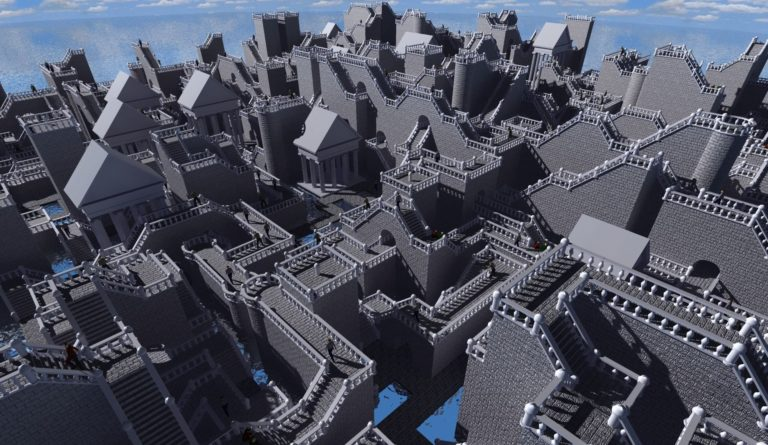
\includegraphics[width=\textwidth, height=0.3\textheight, keepaspectratio]{Images/escher_sample-768x445.jpg}
    \caption{A complex Escheresque tile set that relies on modifying in blocks \cite{model_synthesis_diss}}
    \label{fig:escheresque}
\end{figure}

% Solving these problems is often done in an ad hoc game-specific way that fails to exploit techniques from constraint programming literature.
These issues are rarely addressed directly in implementations. Instead, they are worked around in an ad hoc, game-specific way that fails to exploit constraint programming techniques.

% This work draws an explicit connection between WFC and MAC3 and then presents an implementation in those terms.
Presentation of \acrshort{wfc} online often fails to acknowledge underlying constraint solving principles used by \acrshort{wfc}. Instead, alternative wording is used, which can make forming a deep understanding of the topic challenging.

This dissertation draws an explicit connection between \acrshort{wfc} and the \acrfull{mac3} algorithm, presenting a simple tiled implementation of \acrshort{wfc} in those terms. In simple tiled \acrshort{wfc}, a tile set with adjacency information is used by a constraint solver. This solver attempts to fill a grid of cells with tiles, taking into account their constraints. In the rest of this dissertation, this simple tiled implementation of \acrshort{wfc} is simply referred to as the \acrshort{wfc} algorithm.

% SIMPLE TILED WFC FIGURE
\begin{figure}[H]
    \centering
    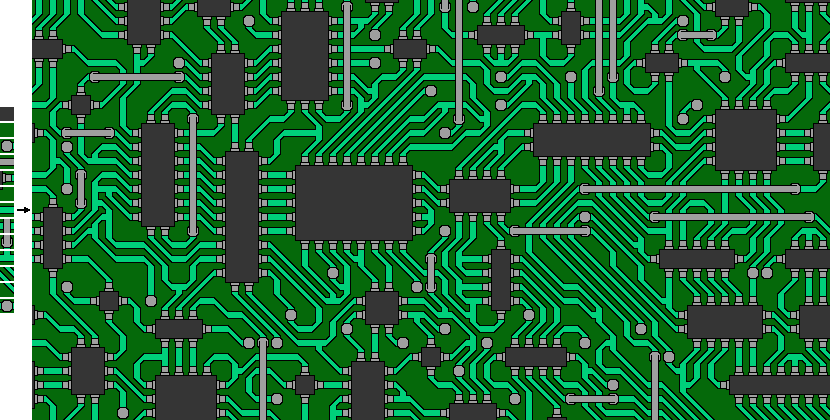
\includegraphics[width=\textwidth, height=0.3\textheight, keepaspectratio]{Images/circuit-1.png}
    \caption{Use of simple tiled \acrshort{wfc} to generate a circuit board graphic \cite{Gumin_Wave_Function_Collapse_2016}}
    \label{fig:WFCcircuit}
\end{figure}

% It also presents:
% An implementation of an extension of WFC that scales world generation infinitely.
% An interface integrated into the Unity game engine for designers to use WFC on their own tilesets.
% A game that utilises the presented techniques.
The simple tiled \acrshort{wfc} implementation is extended using the \acrfull{imib} algorithm, which addresses the challenge of extending \acrshort{wfc} to an infinite space. Furthermore, an interface integrated into the Unity game engine for designers to use \acrshort{wfc} on their own tilesets is included. A simple game themed after \textit{the Backrooms} was created in order to act as an example (Figure \ref{fig:backroomsInGame}).

% In-game screenshot
\begin{figure}[H]
    \centering
    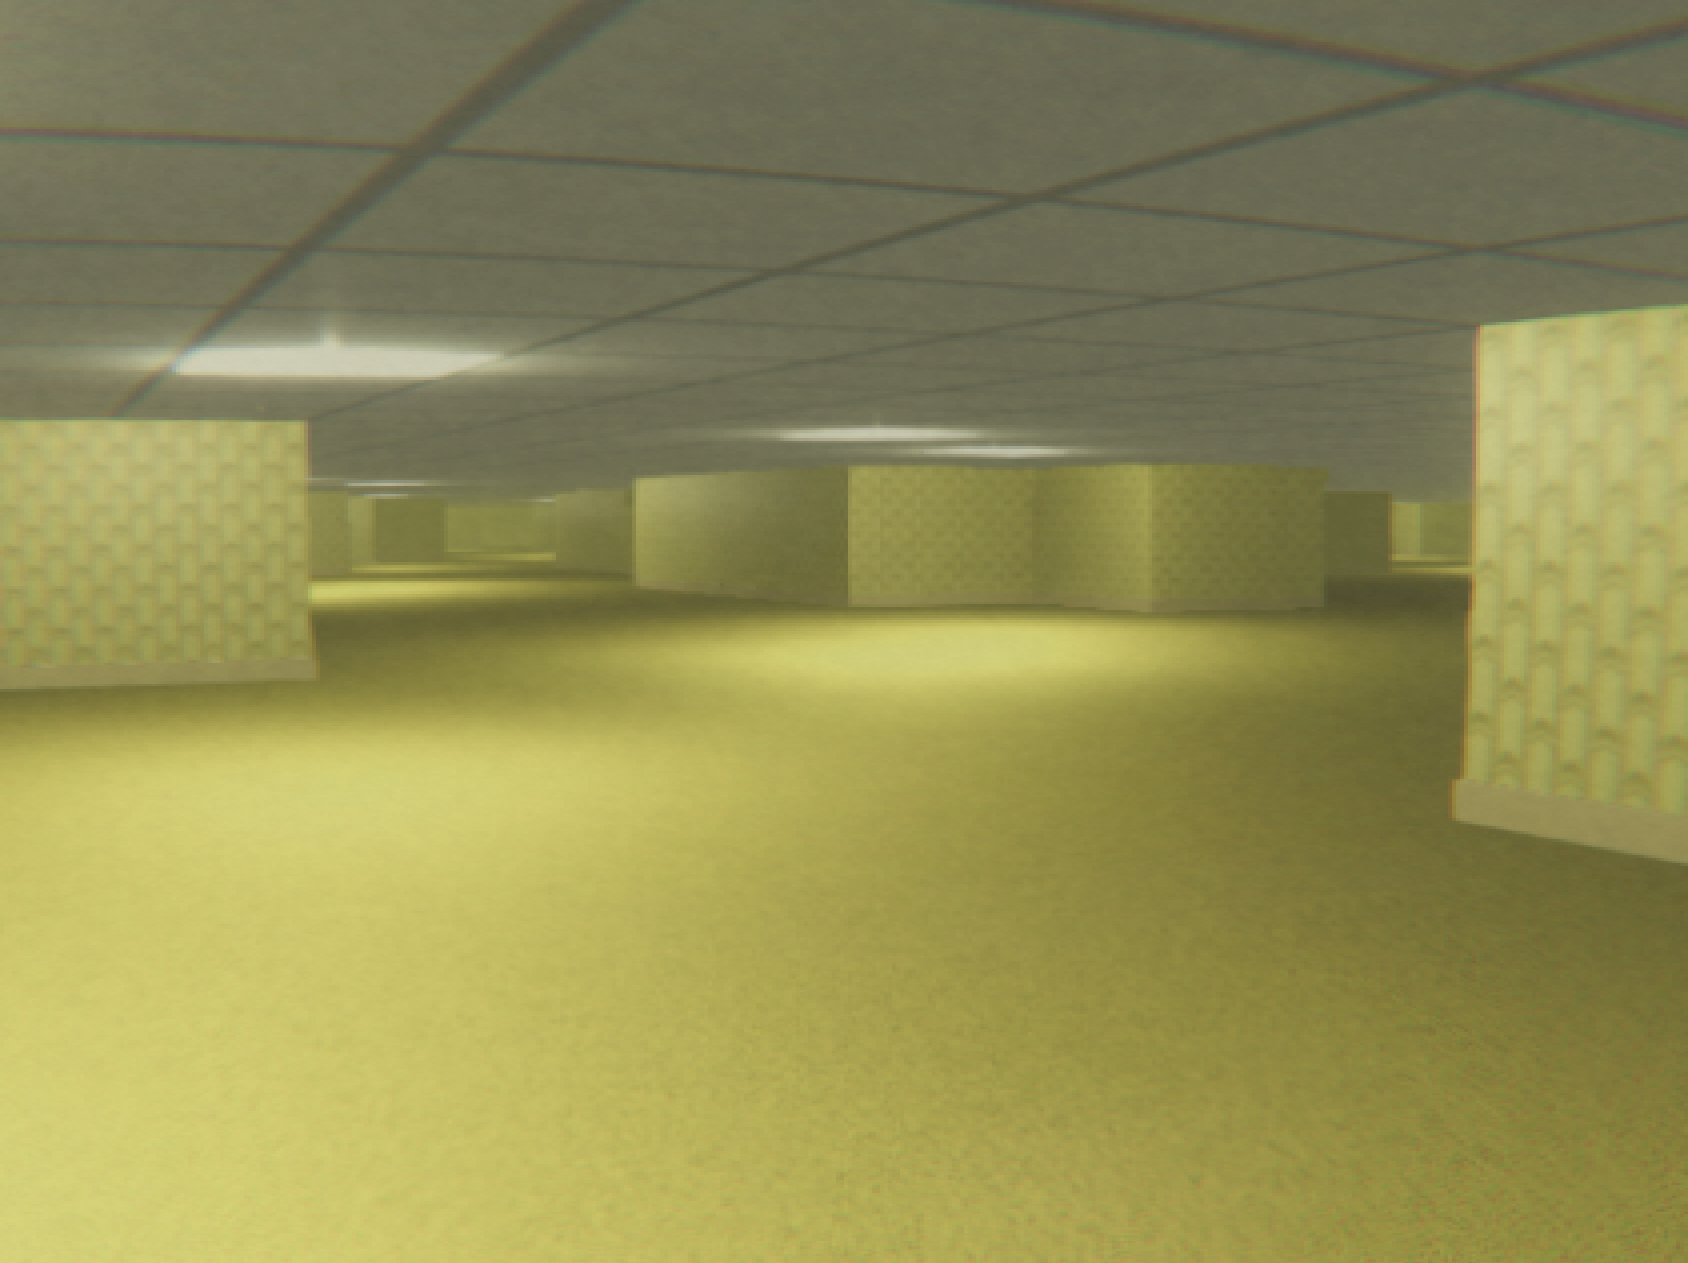
\includegraphics[width=\textwidth, height=0.4\textheight, keepaspectratio]{Images/Backrooms.png}
    \caption{A screenshot from the game}
    \label{fig:backroomsInGame}
\end{figure}


%%%%% OLD INTRODUCTION
% Introduction to the project. Giving background on the areas covered (matching literature review).
%Wave Function Collapse (WFC) is a novel Procedural Content Generation (PCG) technique that has found significant use in video games \cite{Gumin_Wave_Function_Collapse_2016}. WFC can be described as a family of algorithms that enable generation of large game worlds from limited input through the application of constraint programming principles \cite{WFC_ConstraintSolving_and_ML}. This paper applies the simple tiled implementation of WFC, which uses a tile set with adjacency information on how to fit each tile together. The Maintaining Arc Consistency (MAC3) algorithm is then applied to a grid of cells to find a combination of tiles that satisfies adjacency constraints. MAC3 uses concepts of arcs and arc consistency to ensure constraints are satisfied at the start of generation and then maintain satisfaction as tiles to place are chosen. In the rest of the paper, this simple tiled implementation of WFC is simply referred to as the WFC algorithm.

% SIMPLE TILED WFC FIGURE
%\begin{figure}[H]
%\centering
%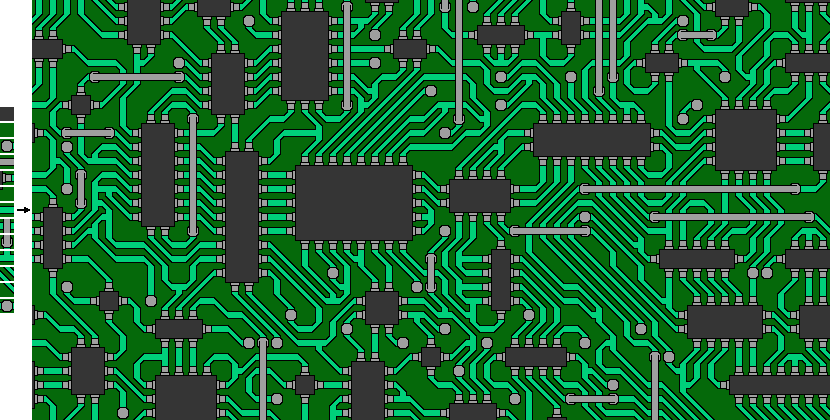
\includegraphics[width=\textwidth, height=0.3\textheight, keepaspectratio]{Images/circuit-1.png}
%\caption{Use of simple tiled WFC to generate a circuit board graphic %\cite{Gumin_Wave_Function_Collapse_2016}}
%\label{fig:WFCcircuit}
%\end{figure}

% Typical practices.
%WFC is often used as a `black box' in a workflow without being altered \cite{WFC_In_The_Wild}. It has had specialised applications in larger workflows in games such as Caves of Qud \cite{cavesofqud}, Townscaper \cite{townscaper} and Bad North \cite{badnorth}. This works around issues like its lack of global constraints, overfitting and performance.

% TOWNSCAPER FIGURE

% Issues to improve upon and how the issues have been addressed.
%One issue with WFC is that complex tile sets and large output areas can present a huge challenge to the constraint solver. In this situation, the solver has a high chance of failing to find a solution without backtracking. The amount of backtracking required can quickly scale with complexity, making just backtracking an infeasible solution. One way that input complexity and output size limitation have been addressed is through the modifying in blocks technique. This was first applied in Model Synthesis, an algorithm that served as inspiration for WFC \cite{model_synthesis}. This breaks the problem down into overlapping blocks that are simpler to evaluate. This generates similar output with a higher chance of success at the cost of additional generation from block overlap.

% ESCHERESQUE FIGURE

% Remaining issues
%One remaining issue is that this generation is on a finite grid. Infinite modifying in blocks addresses this by splitting the world into layers that can be deterministically generated in parallel to create chunks \cite{Infinite_Modifying_In_Blocks}. Parts of this pipeline can be seen in Figure \ref{fig:imib} and are explained in detail in Section \ref{sec:IMIB}. In addition to this, efficient handling of chunk loading and unloading is required. One novel optimisation included the direct calculation of new chunks to load relative to old chunks.

% IMIB FIGURE

% What this projects wants to address in the areas of focus.

% Address how the areas link together.
% Overall aim of the project.
% List of aims as in requirements specification?
% Which aims were achieved and how? Don't have too much detail. This is for the evaluation. % Partially written
\chapter{Literature Review}
% Search for relevant literature
% Evaluate sources
% Identify themes, debates, and gaps
% Outline the structure
% Write your literature review

% Potential Themes:
% Procedural Content Generation
%   Level Generation
%   Randomisation
%   Replayability
%   Search Algorithms
%   Application to AI
%   Image to Image Generation
% Constraint Programming
%   Wave Function Collapse
% Video Games

% Keywords: Video Games, Procedural Content Generation, Wave Function Collapse, Constraint Programming

% What question or problem is the author addressing?
% What are the key concepts and how are they defined?
% What are the key theories, models, and methods?
% Does the research use established frameworks or take an innovative approach?
% What are the results and conclusions of the study?
% How does the publication relate to other literature in the field? Does it confirm, add to, or challenge established knowledge?
% What are the strengths and weaknesses of the research?

% Trends and patterns (in theory, method or results): do certain approaches become more or less popular over time?
% Themes: what questions or concepts recur across the literature?
% Debates, conflicts and contradictions: where do sources disagree?
% Pivotal publications: are there any influential theories or studies that changed the direction of the field?
% Gaps: what is missing from the literature? Are there weaknesses that need to be addressed?

As part of a literature review, three key themes were identified. These include \acrlong{pcg}, Constraint Programming and \acrlong{wfc}. While these themes are presented in three different sections, the ideas discussed heavily overlap.

In summary, constraint programming and \acrlong{pcg} have wide applications and have been a big area of recent research. For example, \acrshort{pcg} has seen increased use of machine learning in recent years, allowing new content to be generated from large dataset models. Similarly, novel constraint programming techniques such as \acrshort{wfc} have seen use in generating new output from very limited input data. These techniques are typically applied to video games in order to help create an ever-changing experience for the player.

\section{Procedural Content Generation}
\subsection{Overview}
\acrshort{pcg} describes the use of algorithms to pseudo-randomly generate content. In the context of video games, this randomisation is often used to provide players with variety that can make games more enjoyable to play multiple times. \acrlong{pcg} can be used in many facets of video game development. One frequent use of \acrshort{pcg} is in randomised level generation. The term `roguelike' is used to describe games where dungeon-style levels are procedurally generated. An example of a roguelike game is \textit{Caves of Qud} \cite{cavesofqud}. How its developers tackled \acrshort{pcg} issues is discussed later in Section \ref{sec:lackOfGlobalConstraints}. In sandbox exploration games such as \textit{Minecraft} \cite{minecraft} and \textit{No Man's Sky} \cite{nomanssky}, \acrshort{pcg} is used to generate the player's world, offering virtually infinite locations to explore. Other uses include randomising enemy characteristics in \textit{Shadow of Mordor} \cite{shadowofmordor} and generating randomised weapons in \textit{Borderlands} \cite{borderlands}. The book \textit{Procedural Content Generation in Games} \cite{pcgbook} is a great resource to read more about \acrshort{pcg}.

\begin{figure}[H]
    \centering
    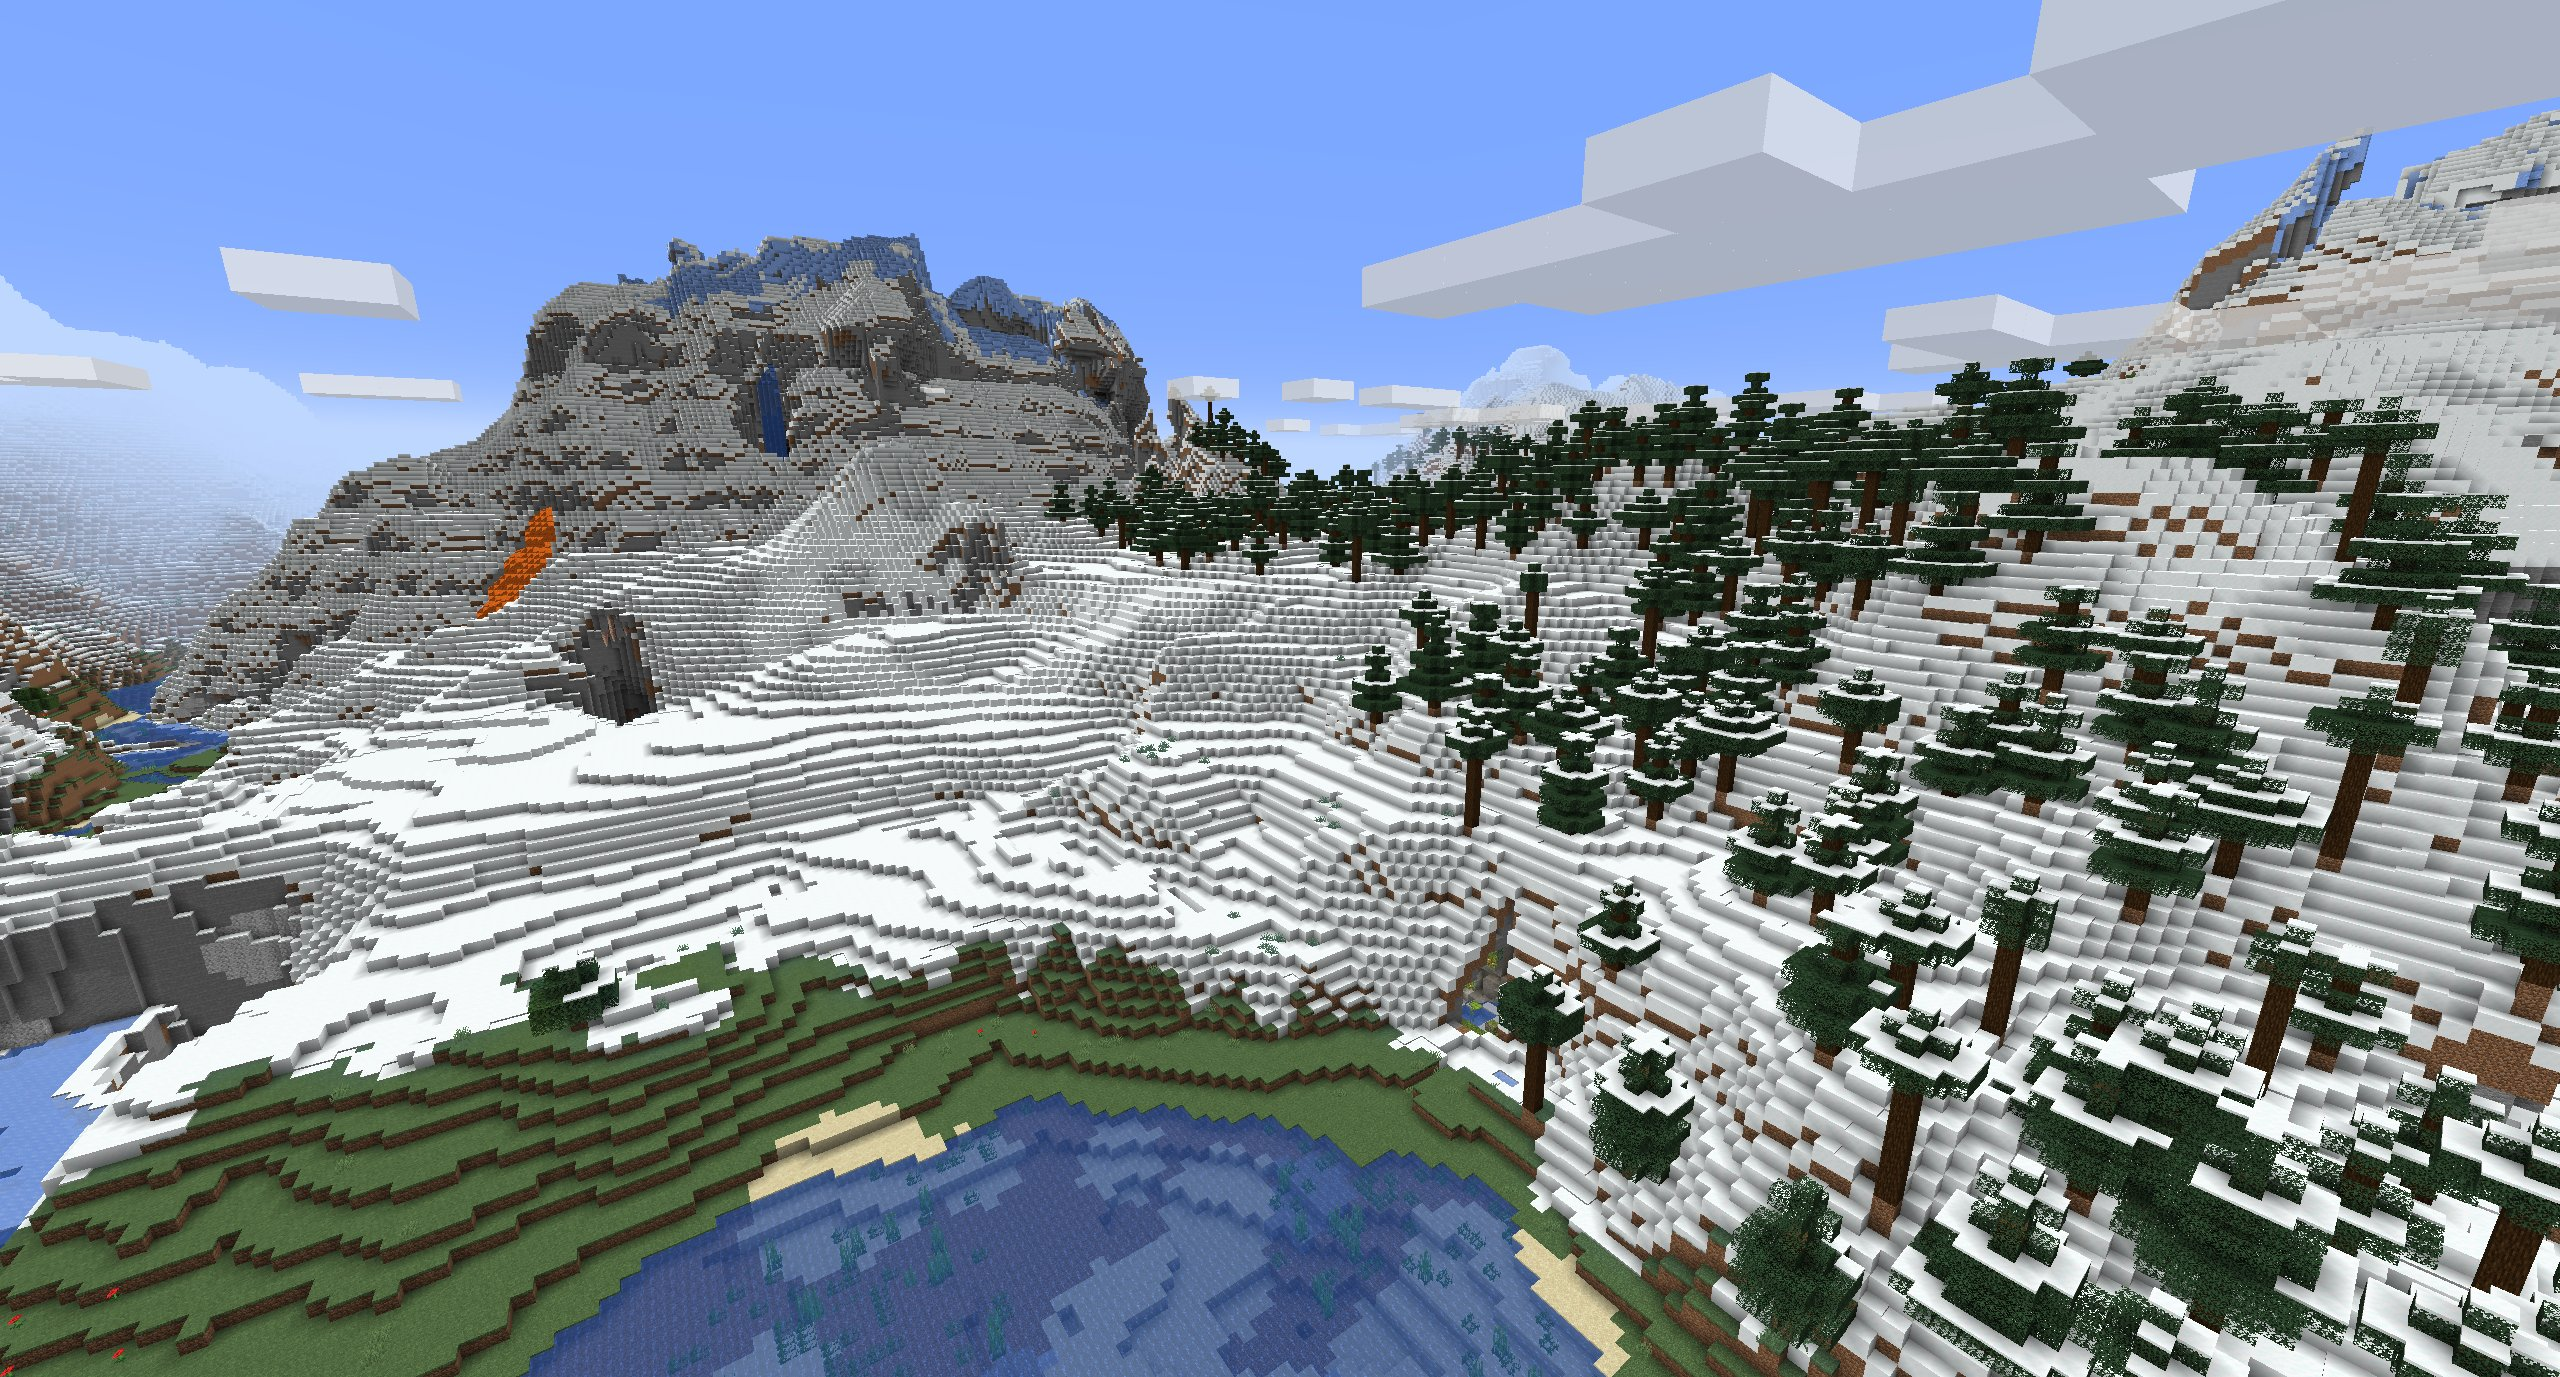
\includegraphics[width=\textwidth, height=0.3\textheight, keepaspectratio]{Images/Minecraft.jpg}
    \caption{\textit{Minecraft} lets the player explore an infinite, procedural world \cite{minecraft_screenshot}}
    \label{fig:minecraftScreenshot}
\end{figure}

\subsection{Current Applications and Research}
Many modern \acrshort{pcg} research looks into using AI and machine learning to generate content. Some current applications of machine learning are art, music and code generation as well as chatbots \cite{AIGC_Survey}, text-to-3D synthesis \cite{Magic3D} and even self-driving cars \cite{Self_Driving_Cars}.

\begin{figure}[H]
    \centering
    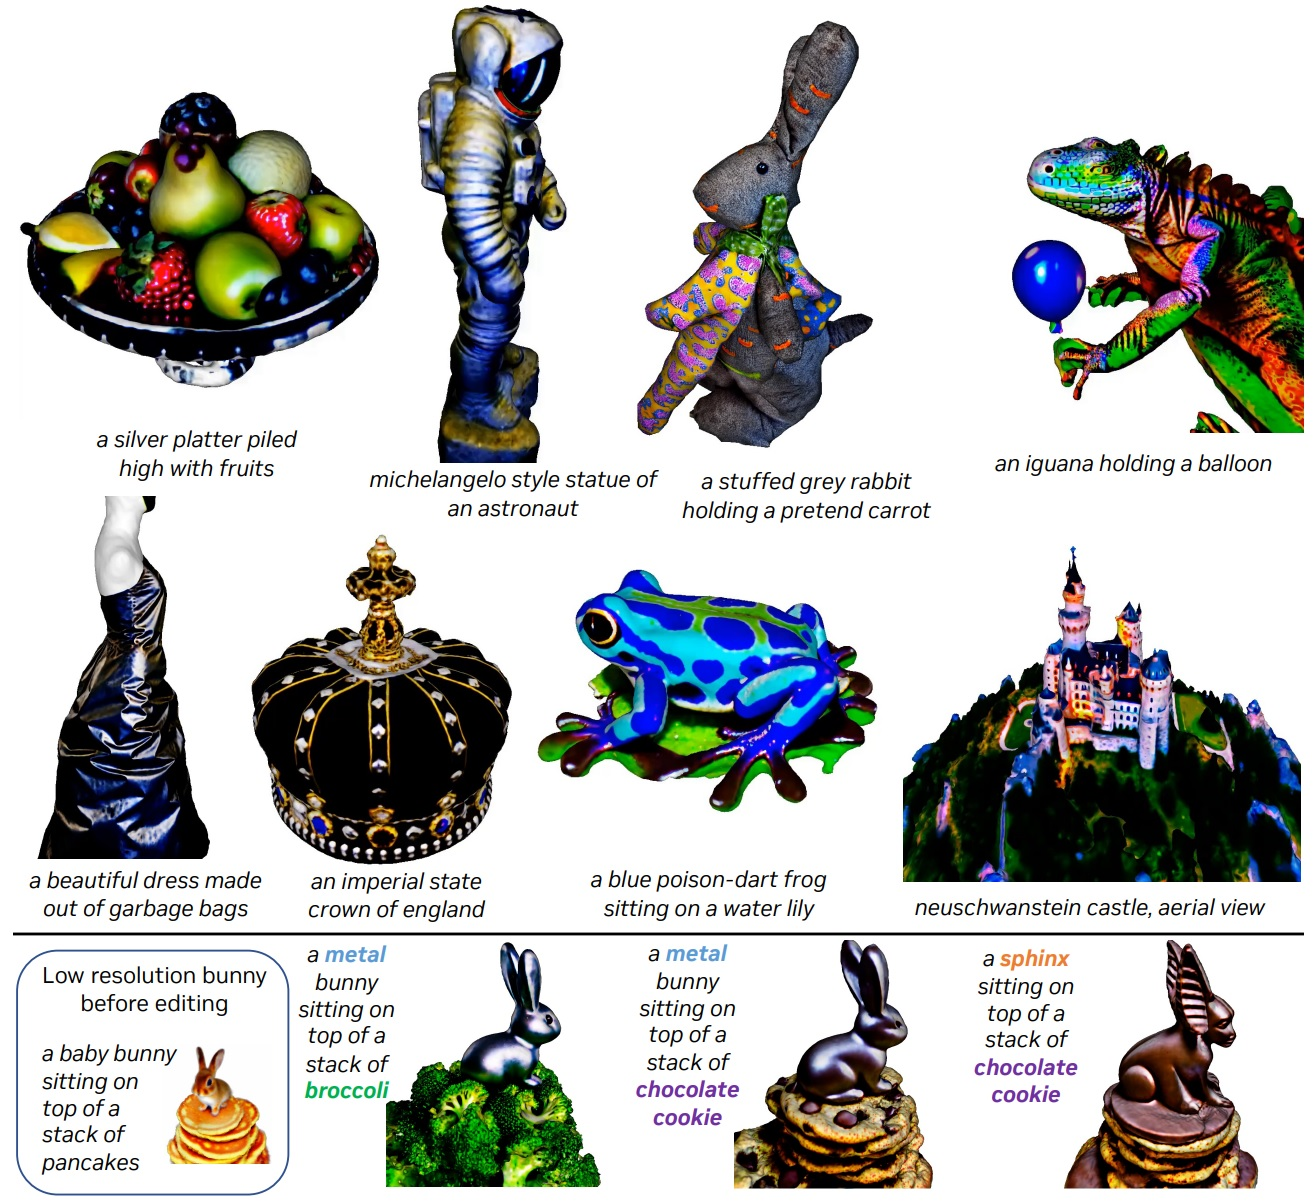
\includegraphics[width=\textwidth, height=0.4\textheight, keepaspectratio]{Images/Magic3D.jpg}
    \caption{Magic3D performs text-to-3D synthesis \cite{Magic3D}}
    \label{fig:magic3D}
\end{figure}

Applications such as Stable Diffusion \cite{Stable_Diffusion} can be used to create high quality text-to-image content (Figure \ref{fig:stableDiffusion}). Others such as Magic3D \cite{Magic3D} offer text-to-3D synthesis (Figure \ref{fig:magic3D}). In terms of text-to-text, ChatGPT \cite{Chat_GPT} serves as a leading language model that can be used to converse about any topic, while GitHub Copilot \cite{GitHub_Copilot} can generate code snippets from user prompts.

\begin{figure}[H]
    \centering
    
\includegraphics[width=\textwidth, height=0.3\textheight, keepaspectratio]{Images/StableDiffusion.jpg}
    \caption{Stable Diffusion offers text-to-image synthesis \cite{Stable_Diffusion}}
    \label{fig:stableDiffusion}
\end{figure}

In the context of games, machine learning is frequently used in areas such as text, character model, texture, music and sound generation \cite{DeepLearningPCG}. Languages such as the Video Game Description Language (VGDL) have even be used to generate entire games using AI (Figure \ref{fig:vgdl}) \cite{VGDL, VGDL_ASP}. However, by themselves, such languages have limited expressiveness, making it difficult to create interesting games \cite{VGDL}.

\begin{figure}[H]
    \centering
    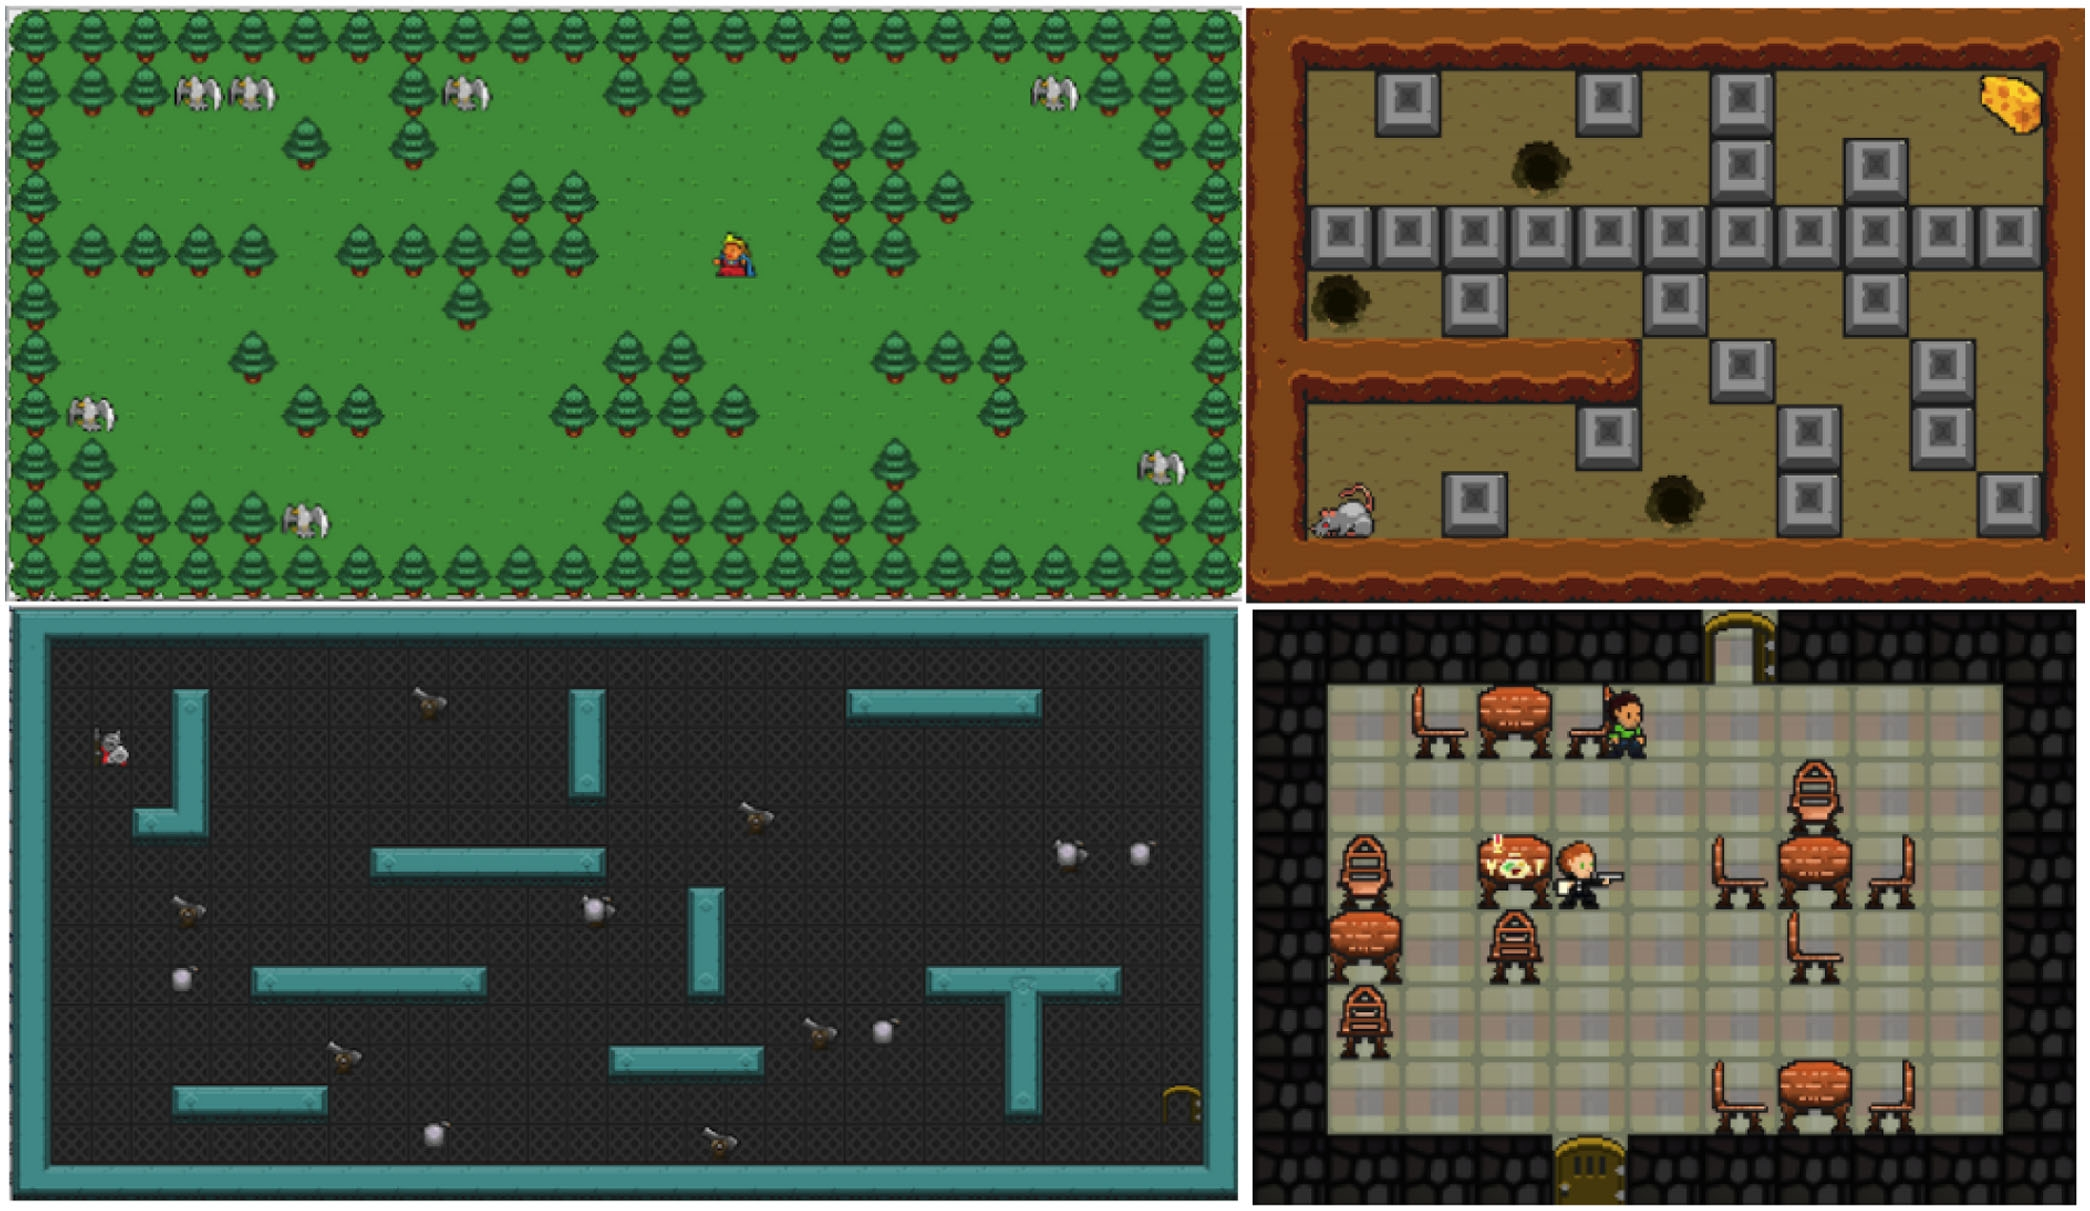
\includegraphics[width=\textwidth, height=0.3\textheight, keepaspectratio]{Images/VGDL.jpg}
    \caption{Games generated using the Video Game Description Language \cite{VGDL}}
    \label{fig:vgdl}
\end{figure}

R. R. Torrado et al. identify that Generative Adversarial Networks (GANs) can also be used for image generation, but that it is difficult to incorporate constraints \cite{CESAGAN}. As a solution, they propose a Conditional Embedding Self-Attention Generative Adversarial Network (CESAGAN). This allows the embedding of a feature vector to the input, enabling the network to model non-local constraints. As a result, this produces higher quality outputs with fewer duplicates as shown in Figure \ref{fig:cesagan}. In \acrshort{wfc}, it is also difficult to enforce non-local constraints without additional modifications.

\begin{figure}[H]
    \centering
    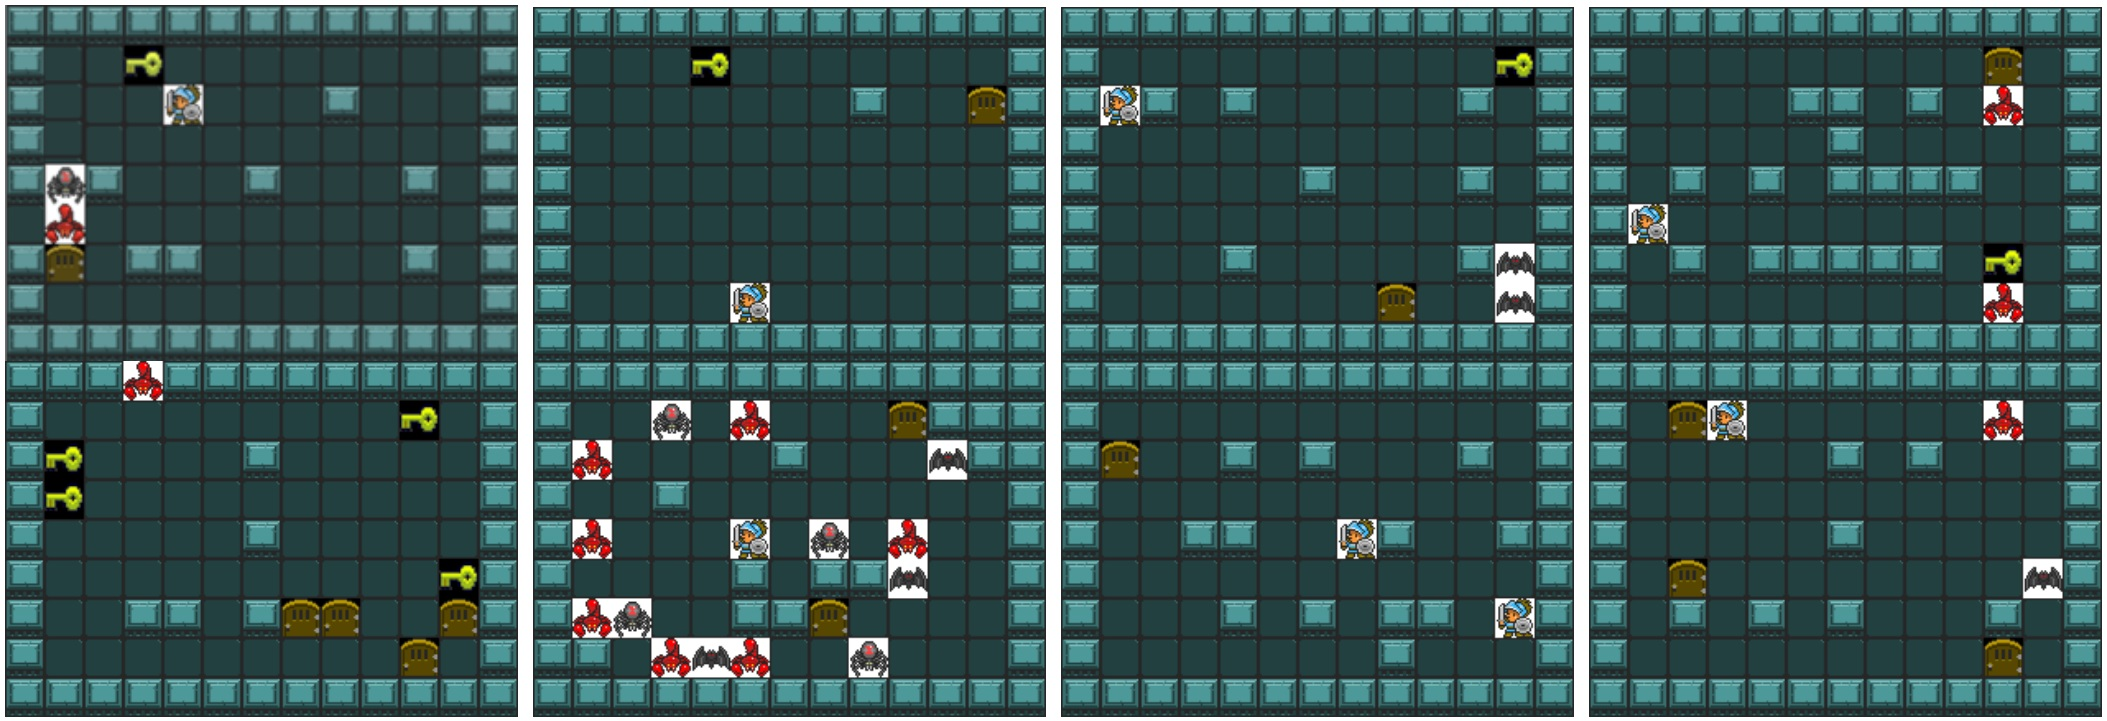
\includegraphics[width=\textwidth, height=0.3\textheight, keepaspectratio]{Images/CESAGAN.jpg}
    \caption{CESAGAN extends upon Generative Adversarial Networks to encourage generation of playable levels requiring additional constraints (top) instead of unplayable levels (bottom) \cite{CESAGAN}}
    \label{fig:cesagan}
\end{figure}

Looking further into machine learning, A. Khalifa et al. transform 2D level design problems into Markov decision processes \cite{Markov_PCGRL}. This approach aids reinforced learning to produce high quality output levels (Figure \ref{fig:pcgrl}). The authors suggest that this reinforced learning could be applied to self-play agents to improve the content generated through simulated playtesting. Three other papers similarly suggest that machine learning is useful for evaluating content through methods such as simulated playtesting \cite{DeepLearningPCG, VGDL_ASP, PCGML}. In the context of \acrshort{wfc}, it might be useful to apply machine learning content evaluation and adjust the output to increase its quality.

\begin{figure}[H]
    \centering
    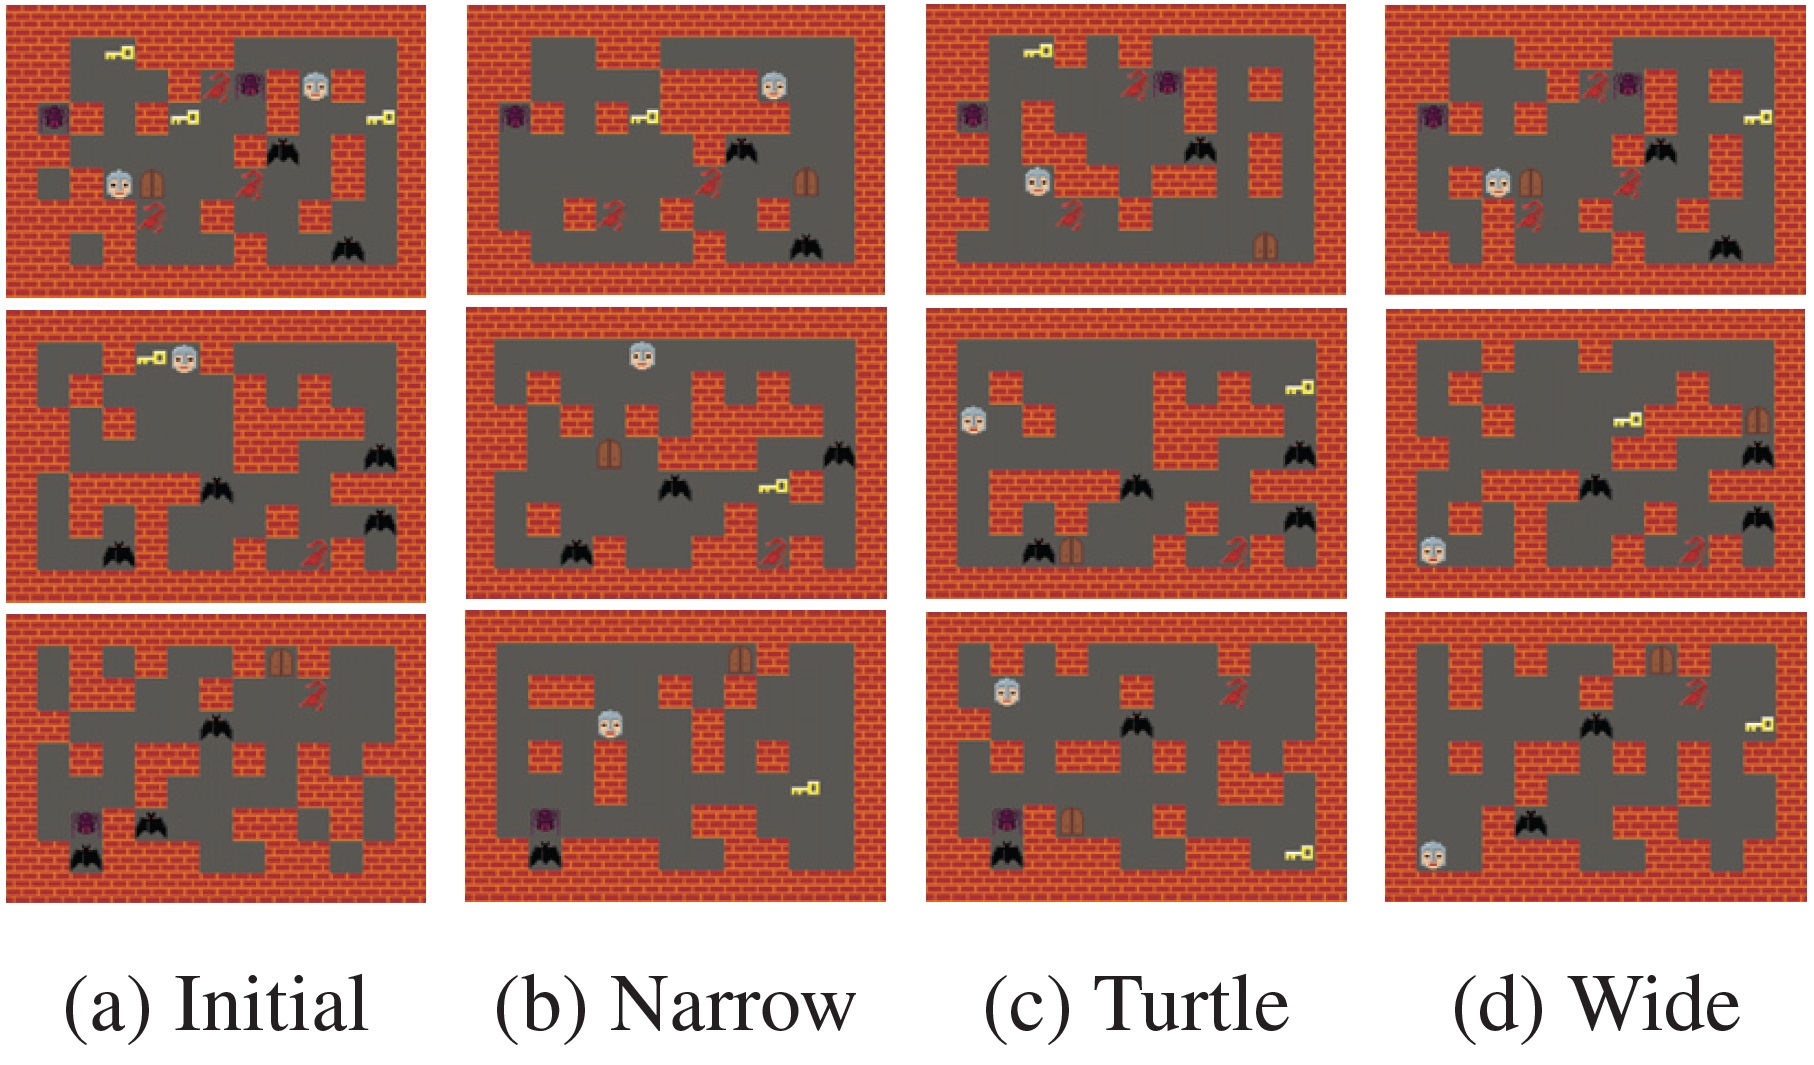
\includegraphics[width=\textwidth, height=0.3\textheight, keepaspectratio]{Images/PCGRL.jpg}
    \caption{\acrlong{pcg} via Reinforcement Learning used to create \textit{Zelda} style levels. An initial random layout (a) is used with three different Markov Decision Process Representations (b), (c) and (d) to create playable levels. \cite{Markov_PCGRL}}
    \label{fig:pcgrl}
\end{figure}

A. Summerville et al. comment specifically on two limitations of \acrshort{pcg} via machine learning \cite{PCGML}. They state that the playability of output produced through machine learning is not guaranteed to be playable, but rather biassed towards generating playable content through the input. Similarly, whether \acrshort{wfc} output is playable or not is not always guaranteed but heavily depends on how the input is defined. As a result, both machine learning \acrshort{pcg} and \acrshort{wfc} require carefully tweaked input data and an output evaluator when applied to level generation. The second limitation is that most machine learning has been applied to 2D content. Once again, the core \acrshort{wfc} implementation and many of its offshoots exhibit the same limitation of only supporting 2D content generation \cite{Gumin_Wave_Function_Collapse_2016}. Investigating further, A. Summerville et al. present a taxonomisation of \acrlong{pcg} Machine Learning techniques, shown in Figure \ref{fig:pcgml}.

\begin{figure}[H]
    \centering
    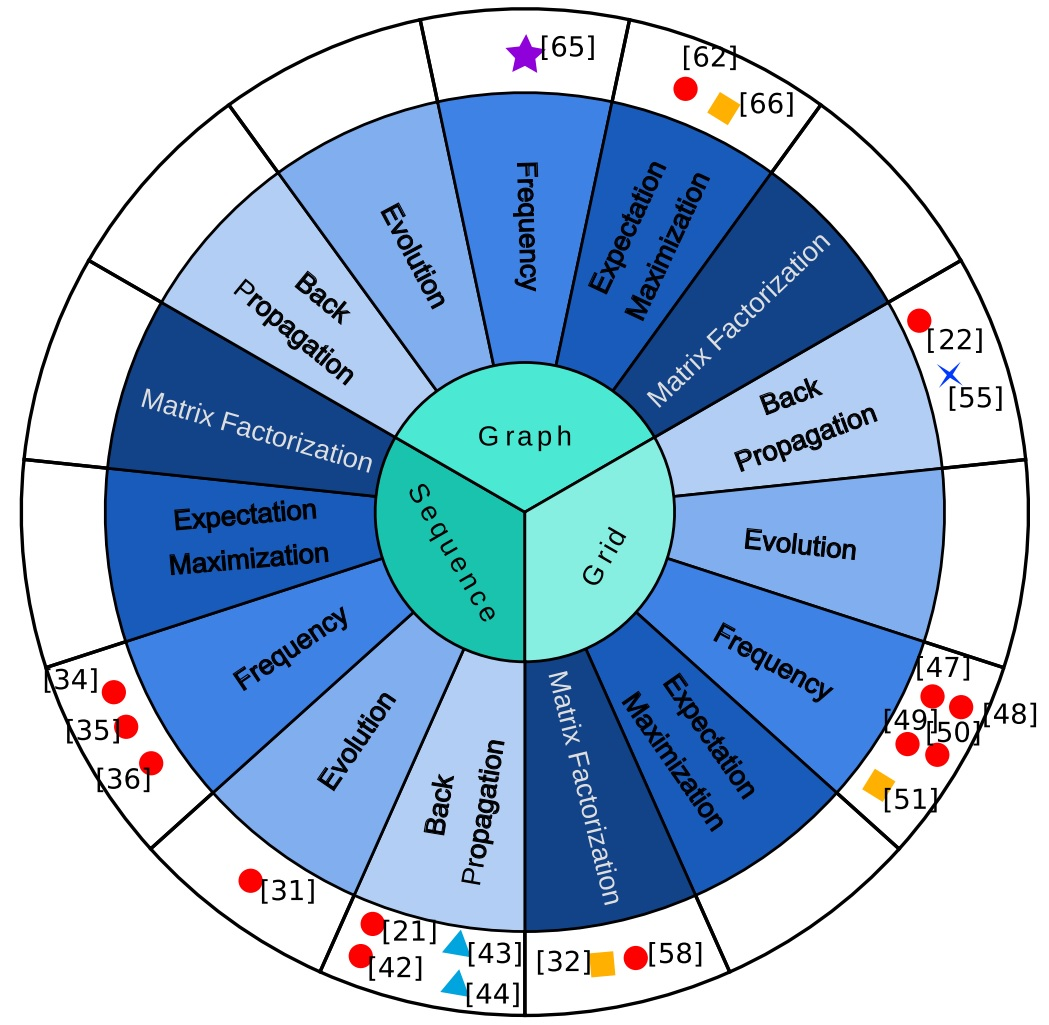
\includegraphics[width=\textwidth, height=0.5\textheight, keepaspectratio]{Images/PCGMLTaxonomy.jpg}
    \caption{A taxonomisation of \acrlong{pcg} Machine Learning techniques. There are two categorisations: the underlying data structure (graph, grid, or sequence) and the training method (matrix factorisation, EM, frequency counting, evolution, and backpropagation). Marks are colored for the specific type of content that was generated: red circles are platformer levels, orange squares are ``dungeons,'' the dark blue x is real time strategy levels, light blue triangles are collectible game cards, and the purple star is interactive fiction. Citations for each are listed. Citation numbers correspond to those in the cited paper. \cite{PCGML}}
    \label{fig:pcgml}
\end{figure}



\section{Constraint Programming}
\subsection{Overview}
% Introduce CP and discuss some of the problems that it tackles.
Constraint programming deals with modelling problems through constraints and then running a solver to find solutions. In the context of \acrshort{pcg} and video games, the use of constraints can be useful to tailor the output of \acrshort{pcg} as desired and generate new content based on old content. Constraint programming has also been used to solve game tasks. The use of constraints allows for well-defined outputs to be created, but pay for this with more unpredictable generation times when compared to other methods \cite{WFC_In_The_Wild}. Furthermore, constraint programming has been applied to a large variety of problem categories, ranging from combinatorial mathematics to logistics and scheduling \cite{CSPLib}.

% Then discuss some current research and identify which problems they attempt to solve.
\subsection{Combinatorial Problems}
Q. Cappart et al. take a deeper look into combinatorial problems. These problems deal with finding an optimal solution among a finite set of possibilities. The authors acknowledge that deep reinforcement learning has been used to tackle these problems, but that it only provides approximate solutions \cite{Combinatorics_CP_RL}. To find optimal solutions, they combine deep RL with constraint programming, detailing its use for problems such as the travelling salesman problem with time windows and the 0-1 knapsack problem.

P. Spracklen et al. comment that large scale combinatorial problems may have huge search spaces, resulting in low solver performance \cite{Combinatorics_Streamliner_Constraints}. To address this, they introduce an automated process to add streamliner constraints, which focus effort on searching promising parts of the search space to improve performance.

Furthermore, a survey of combinatorial problems and attempts at modelling and solving them effectively identifies, for example, that algorithm selection techniques can achieve significant performance improvements for combinatorial search \cite{Data_Mining_and_Constraint_Programming}. The survey presents a model for the algorithm selection problem, shown in Figure \ref{fig:algorithmSelection}.

\begin{figure}[H]
    \centering
    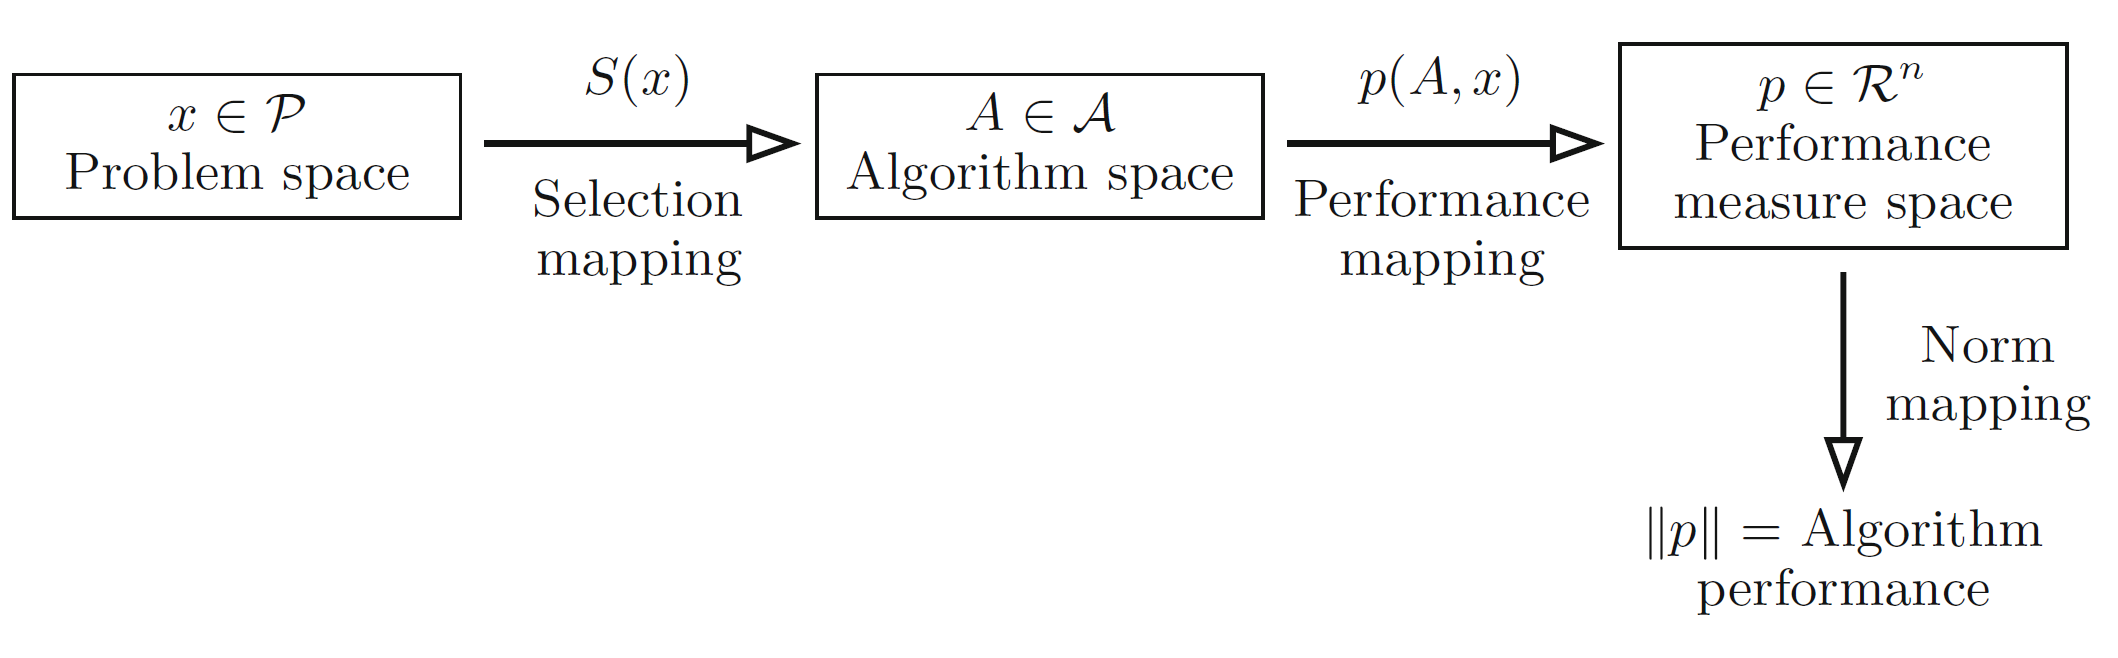
\includegraphics[width=\textwidth, height=0.3\textheight, keepaspectratio]{Images/AlgorithmSelection.png}
    \caption{Basic model for the Algorithm Selection Problem \cite{Data_Mining_and_Constraint_Programming}}
    \label{fig:algorithmSelection}
\end{figure}

Ö. Akgün et al. recognise the difficulty in testing constraint solvers due to the vastness of searches they may perform \cite{Metamorphic_Testing}. As a solution, they use metamorphic testing, which generates new test cases from existing ones. However, they also express the limitation that this should be used with other forms of testing. The authors state that this is because metamorphic testing does not recognise when a solver falsely identifies a problem as unsolvable.

\subsection{Logic Programming Languages}
Another interesting application of constraint programming is to AI deep reinforced learning. G. De Gasperi et al. explore the use of the Prolog logic programming language to generate data sets to aid this learning, finding positive results in trained AI agent performance \cite{Prolog_Deep_Learning}. As part of this process, they convert user-specified constraints into Prolog queries through a Python program that generates JSON house plans (Figure \ref{fig:housePlans}). The pipeline for this is shown in Figure \ref{fig:pythonToProlog}.

\begin{figure}[H]
    \centering
    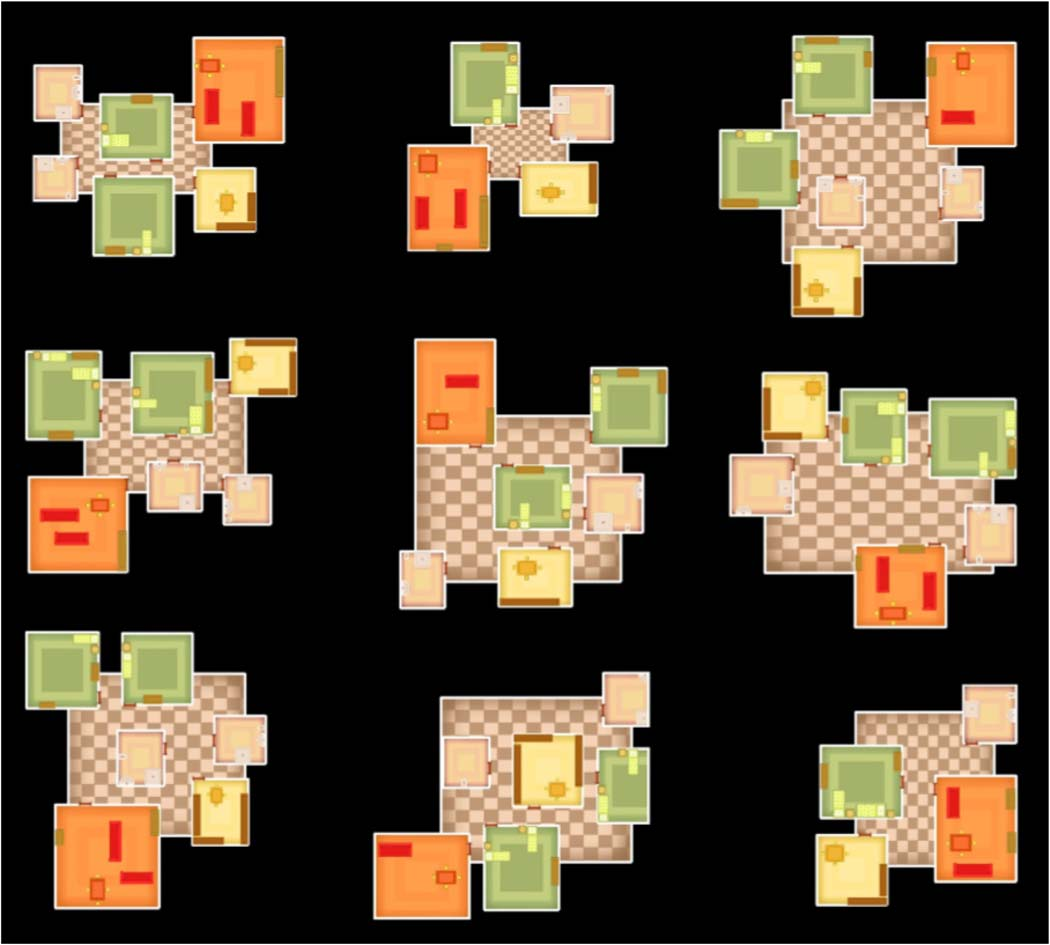
\includegraphics[width=\textwidth, height=0.3\textheight, keepaspectratio]{Images/HousePlans.jpg}
    \caption{Examples of generated house plans \cite{Prolog_Deep_Learning}}
    \label{fig:housePlans}
\end{figure}

\begin{figure}[H]
    \centering
    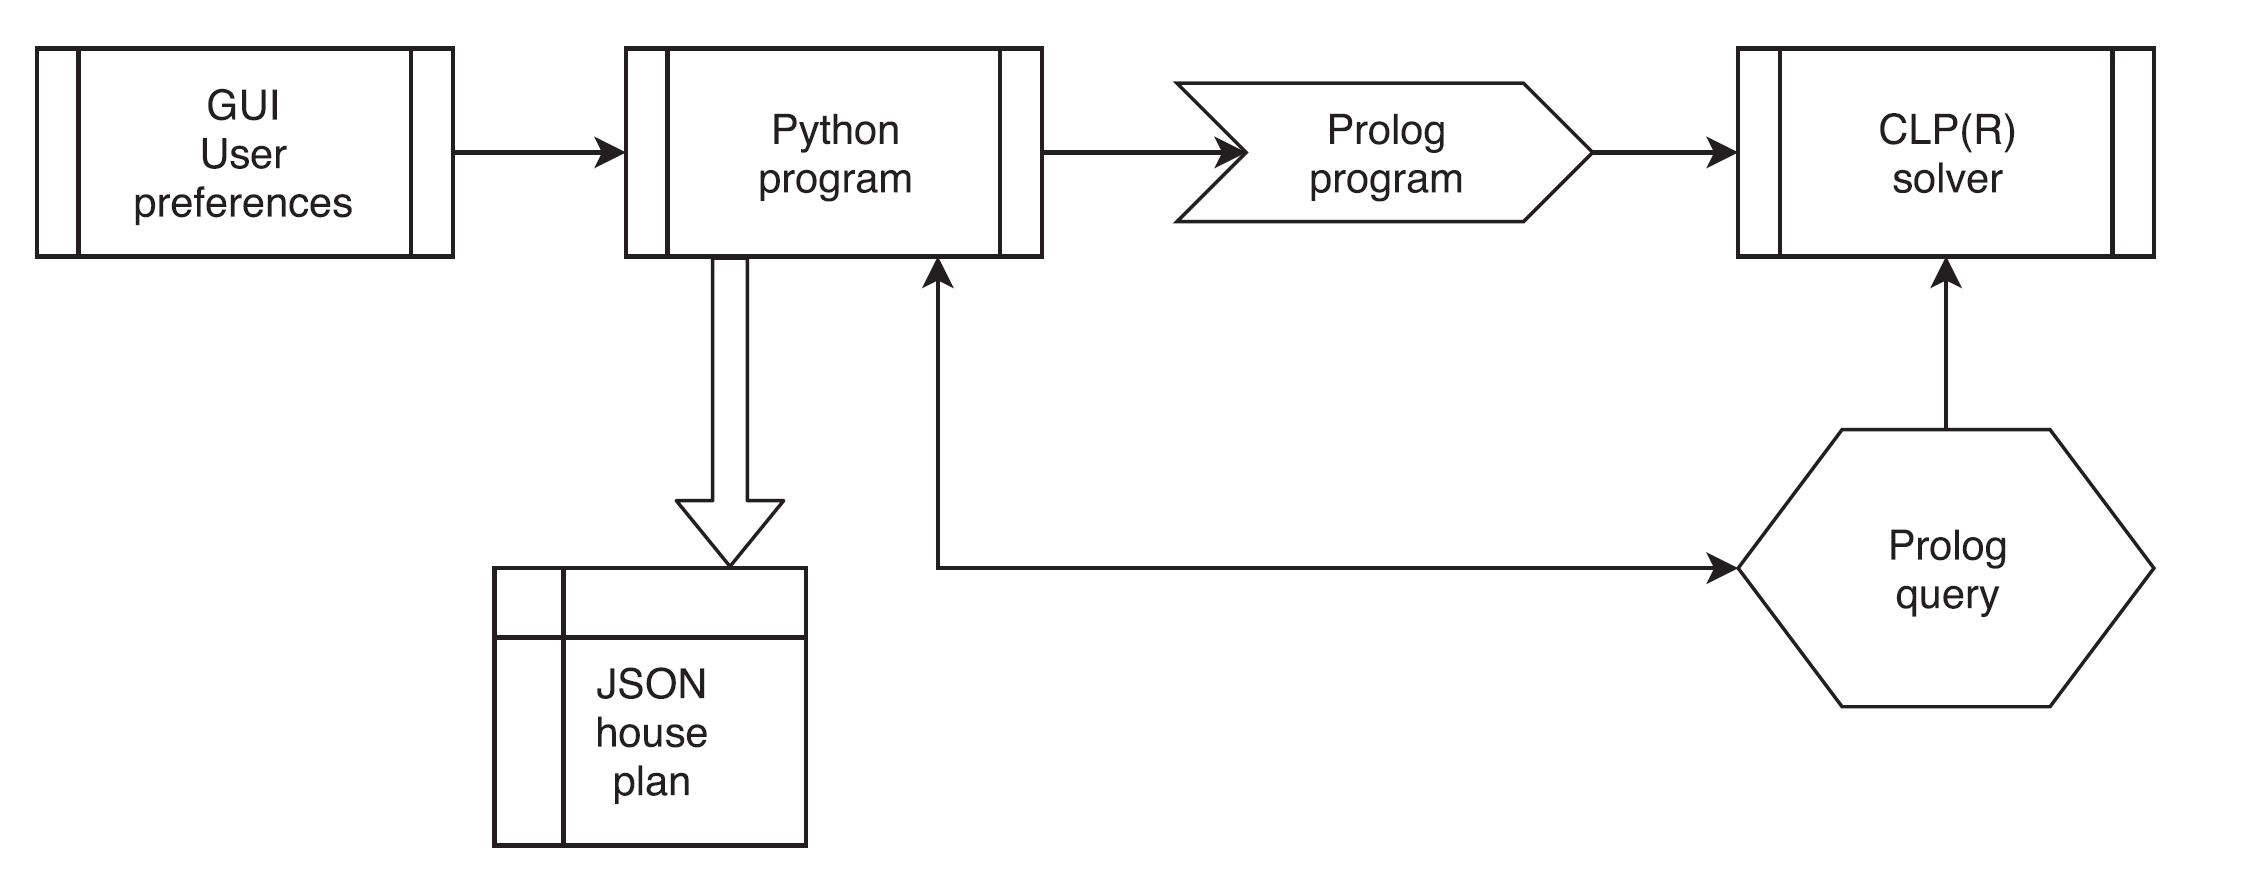
\includegraphics[width=\textwidth, height=0.3\textheight, keepaspectratio]{Images/PythonToProlog.png}
    \caption{Python converting user-specified constraints into Prolog queries \cite{Prolog_Deep_Learning}}
    \label{fig:pythonToProlog}
\end{figure}

Other languages similar to Prolog, such as Answer Set Programming (ASP) and the Video Game Description Language (VGDL), extend Prolog's concepts with application to video games. For example, ASP can be used to generate constrained dungeons (Figure \ref{fig:aspDungeons}) \cite{pcgbook}. A range of constraints are encoded. Altars (the golden A tiles) are constrained to have four empty tiles around them. Wall tiles must have at least two neighbouring walls, encouraging the formation of larger wall segments. Gems (the green G tiles) must have three adjacent walls, making them stuck in wall segments. Finally, there must be a path with a minimum length between altars and gems, as well as a path diagonally across the level through this. All of these constraints work together to generate interesting, playable levels.

\begin{figure}[H]
    \centering
    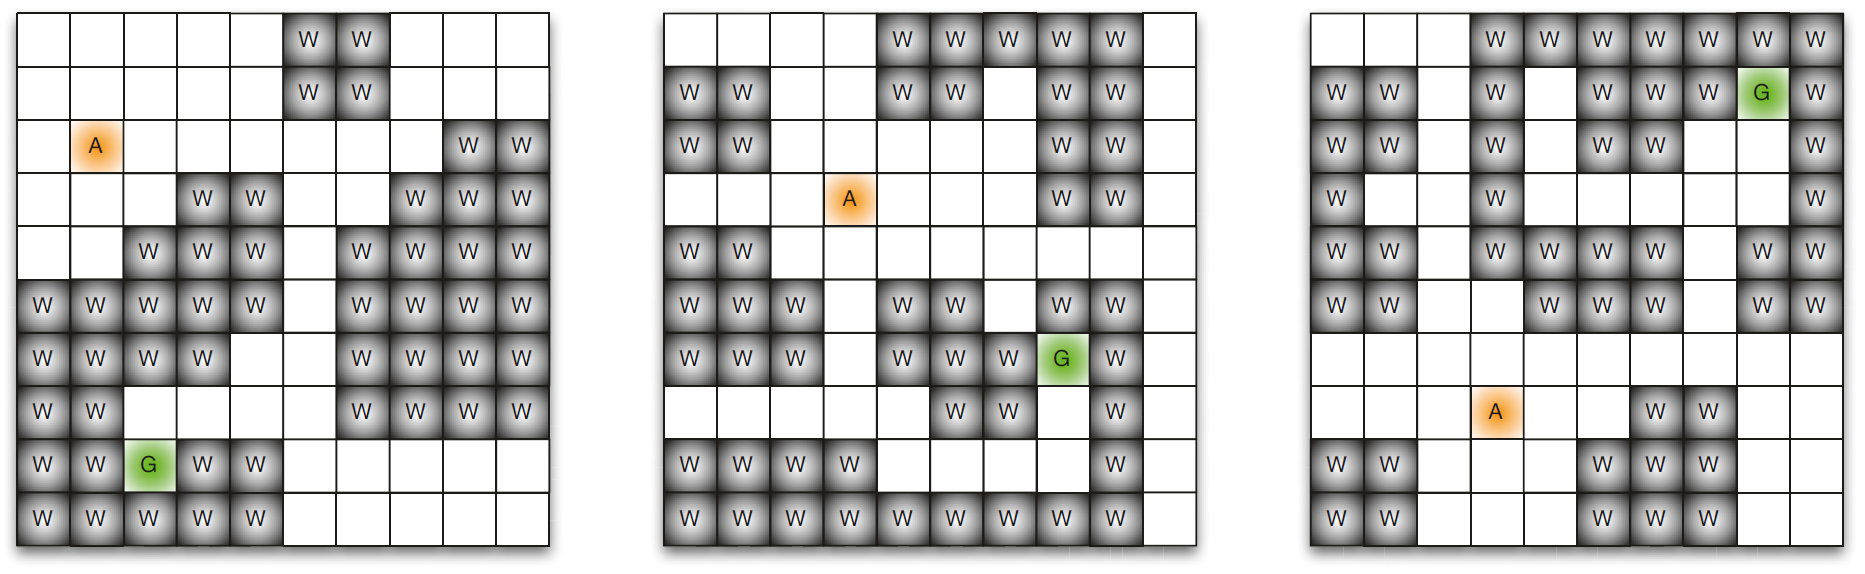
\includegraphics[width=\textwidth, height=0.3\textheight, keepaspectratio]{Images/ASPDungeons.png}
    \caption{Examples of dungeons generated using ASP \cite{pcgbook}}
    \label{fig:aspDungeons}
\end{figure}

G. Glorian et al. also apply constraint programming to dungeon generation, but instead use a graph constraint to generate high quality dungeons with distinct areas \cite{Graph_Constraint_Dungeon}. Hundreds of variations can be generated from one dungeon with labelled rooms. The dungeon is represented as a graph, which lets areas be selectively turned off and rearranged while meeting design constraints. The concept is shown in Figure \ref{fig:graphDungeon}.

\begin{figure}[H]
    \centering
    \subfigure[The full dungeon]{
        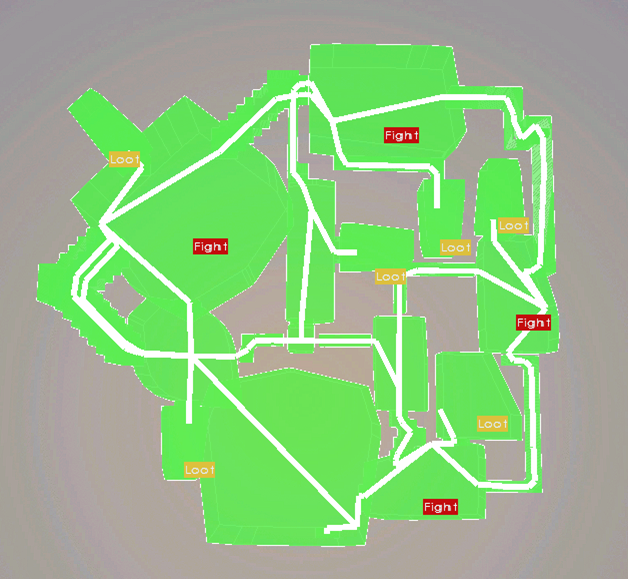
\includegraphics[width=0.475\textwidth, height=0.35\textheight, keepaspectratio]{Images/GraphDungeon1.png}
        \label{fig:graphDungeon1}
    }
    \hfill
    \subfigure[One variation]{
        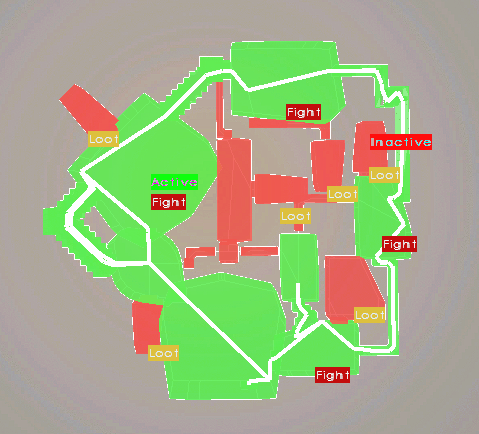
\includegraphics[width=0.475\textwidth, height=0.35\textheight, keepaspectratio]{Images/GraphDungeon2.png}
        \label{fig:graphDungeon2}
    }
    \caption{Generating a variation from a larger dungeon \cite{Graph_Constraint_Dungeon}}
    \label{fig:graphDungeon}
\end{figure}

A. Khalifa et al. build on the General Video Game AI framework (GVG-AI) and the Video Game Description Language (VGDL) to create general video game generators \cite{GVG-AI_and_VGDL_Level_Generators}. These generators aim to save time by eliminating the need to custom-build a generator for each game. Instead, a game description is given as input and used to generate a level for the game. The results of three generators for a \textit{Zelda}-style game are shown in Figure \ref{fig:gvgAILevels}. Here, the aim is to collect the key and get to the exit while avoiding attacks by monsters. The player has a sword that can be used to attack monsters and gain additional points.

\begin{figure}[H]
    \centering
    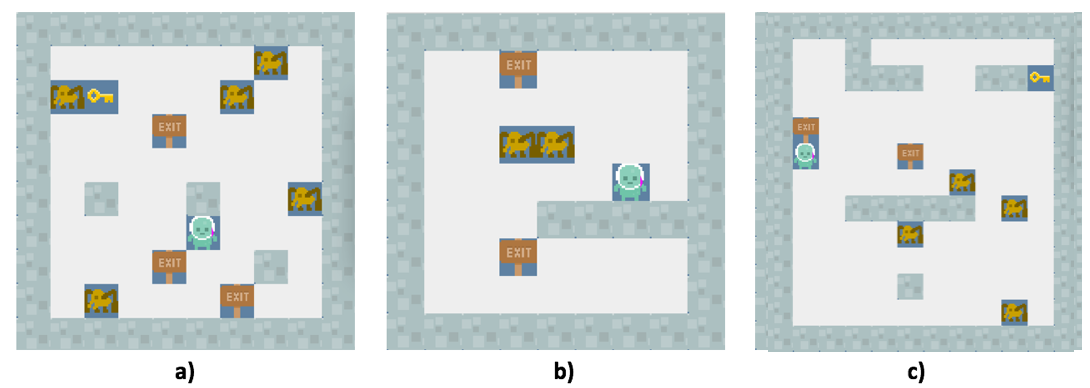
\includegraphics[width=\textwidth, height=0.3\textheight, keepaspectratio]{Images/GVGAILevels.png}
    \caption{\textit{Zelda}-style levels being generated by a Random Level Generator (a), Constructive Level Generator (b) and Search-Based Level Generator (c) \cite{GVG-AI_and_VGDL_Level_Generators}}
    \label{fig:gvgAILevels}
\end{figure}

\subsection{Further Application to Video Games}
In the context of video games, constraint programming research has looked into applying constraints to \acrshort{pcg} and solving game tasks. J. Espasa et al. aimed to solve a planning problem presented in the game \textit{Plotting} \cite{Plotting_Planning_Problem}. In \textit{Plotting}, the player must plan a sequence of actions to clear blocks of varying types from a grid. The authors model the problem in two modelling language, namely the widely used Planning Domain Definition Language (PDDL) and the novel Essence Prime. Their effectiveness is then compared using several solvers, finding a SAT solver to be most effective for the problem as shown in Figure \ref{fig:plottingSolverComparison}.

\begin{figure}[H]
    \centering
    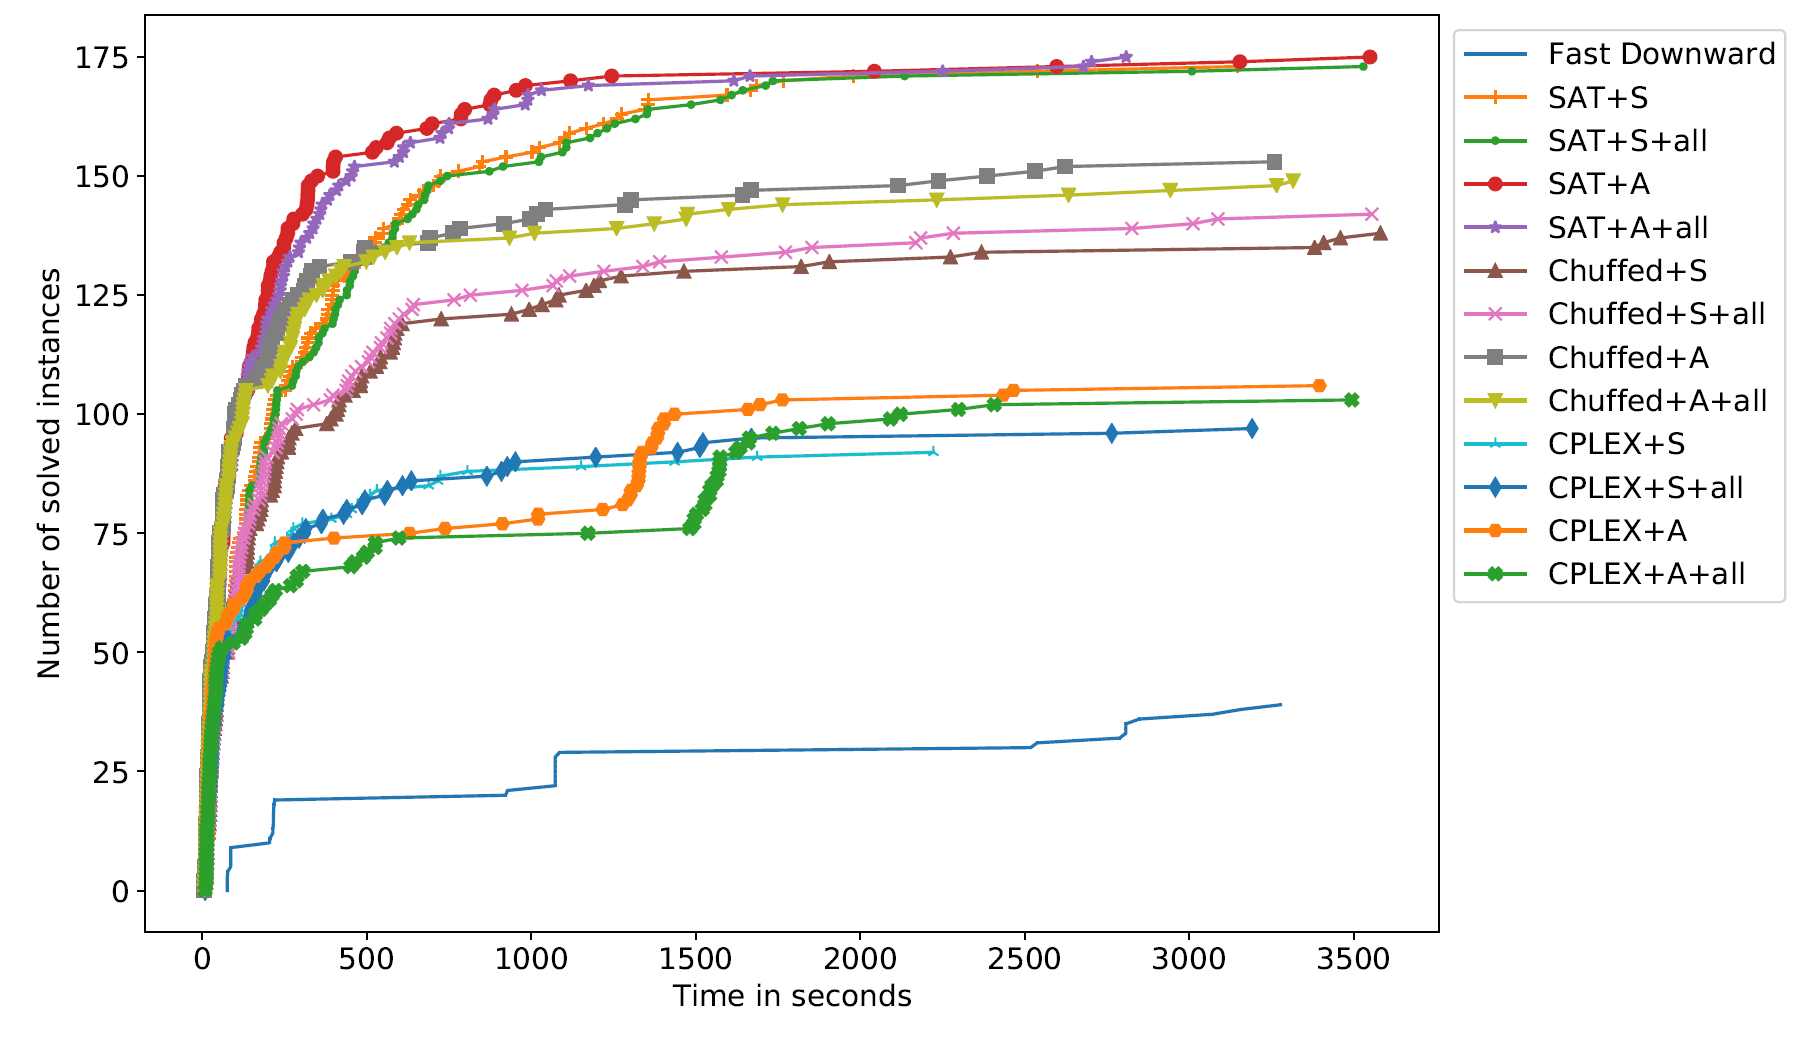
\includegraphics[width=\textwidth, height=0.3\textheight, keepaspectratio]{Images/PlottingSolverComparison.png}
    \caption{Comparing performance of \textit{Plotting} models and solvers \cite{Plotting_Planning_Problem}}
    \label{fig:plottingSolverComparison}
\end{figure}

%\subsection{Constraint Types}
%\subsubsection{Global}
%\subsubsection{Local}

\section{Wave Function Collapse}
\acrshort{wfc} \cite{Gumin_Wave_Function_Collapse_2016} is a modern \acrshort{pcg} method that has found use in games such as \textit{Townscaper} \cite{townscaper} and \textit{Bad North} \cite{badnorth}. It can be described as a family of algorithms, rather than one specific algorithm \cite{WFC_ConstraintSolving_and_ML}. As such, a large variety of implementations are available online, each with their own specialisations to solve the problem for which they were designed. I. Karth and A. M. Smith note that \acrshort{wfc} is often used as a black box, being incorporated into a workflow without being altered \cite{WFC_In_The_Wild}.

\begin{figure}[H]
    \centering
    
\includegraphics[width=\textwidth, height=0.3\textheight, keepaspectratio]{Images/BadNorth.jpg}
    \caption{\textit{Bad North} uses \acrshort{wfc} to generate islands traversable by AI \cite{badnorth}}
    \label{fig:badNorth}
\end{figure}

\acrshort{wfc} builds off of the concepts of Model Synthesis, which is a method for procedurally modelling complex 3D shapes \cite{model_synthesis, model_synthesis_diss}. In Model Synthesis, the user defines an input model detailing various dimensional, geometric and algebraic constraints. This is then used to create output satisfying the modelled constraints. A simple example using a pillar model is shown in Figure \ref{fig:modelSynthesis}.

\begin{figure}[H]
    \centering
    \subfigure[An input model with model pieces arranged and labelled 0 to 3]{
        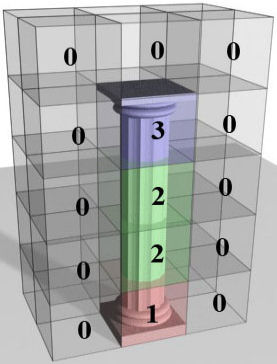
\includegraphics[width=0.475\textwidth, height=0.3\textheight, keepaspectratio]{Images/ModelSynthesis1.jpg}
        \label{fig:modelSynthesis1}
    }
    \hfill
    \subfigure[Pillar variations using the input model pieces]{
        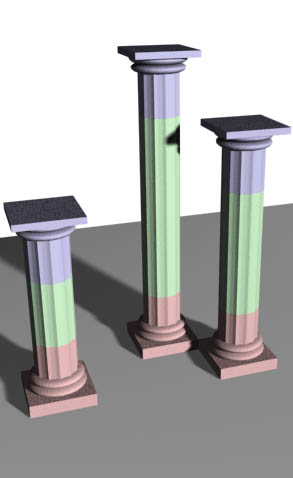
\includegraphics[width=0.475\textwidth, height=0.3\textheight, keepaspectratio]{Images/ModelSynthesis2.jpg}
        \label{fig:modelSynthesis2}
    }
    \caption{Generating pillars of different lengths from input model pieces \cite{model_synthesis_diss}}
    \label{fig:modelSynthesis}
\end{figure}

\subsection{Implementation Variations}
\subsubsection{Data Input}
The data input stage is likely the \acrshort{wfc} stage with the most variation across implementations. The original implementation \cite{Gumin_Wave_Function_Collapse_2016} supports both an overlapping and simple tiled model. The overlapping version takes a sample image and defines overlapping patterns of \(N\times N\) tiles, where the output is constructed of a random arrangement of these patterns. The overlapping \acrshort{wfc} pipeline is shown in Figure \ref{fig:overlappingWFC}. The simple tiled model instead defines single tile patterns, where each tile has its own defined set of possible neighbours. An example of simple tiled generation was shown in Figure \ref{fig:WFCcircuit}.

\begin{figure}[H]
    \centering
    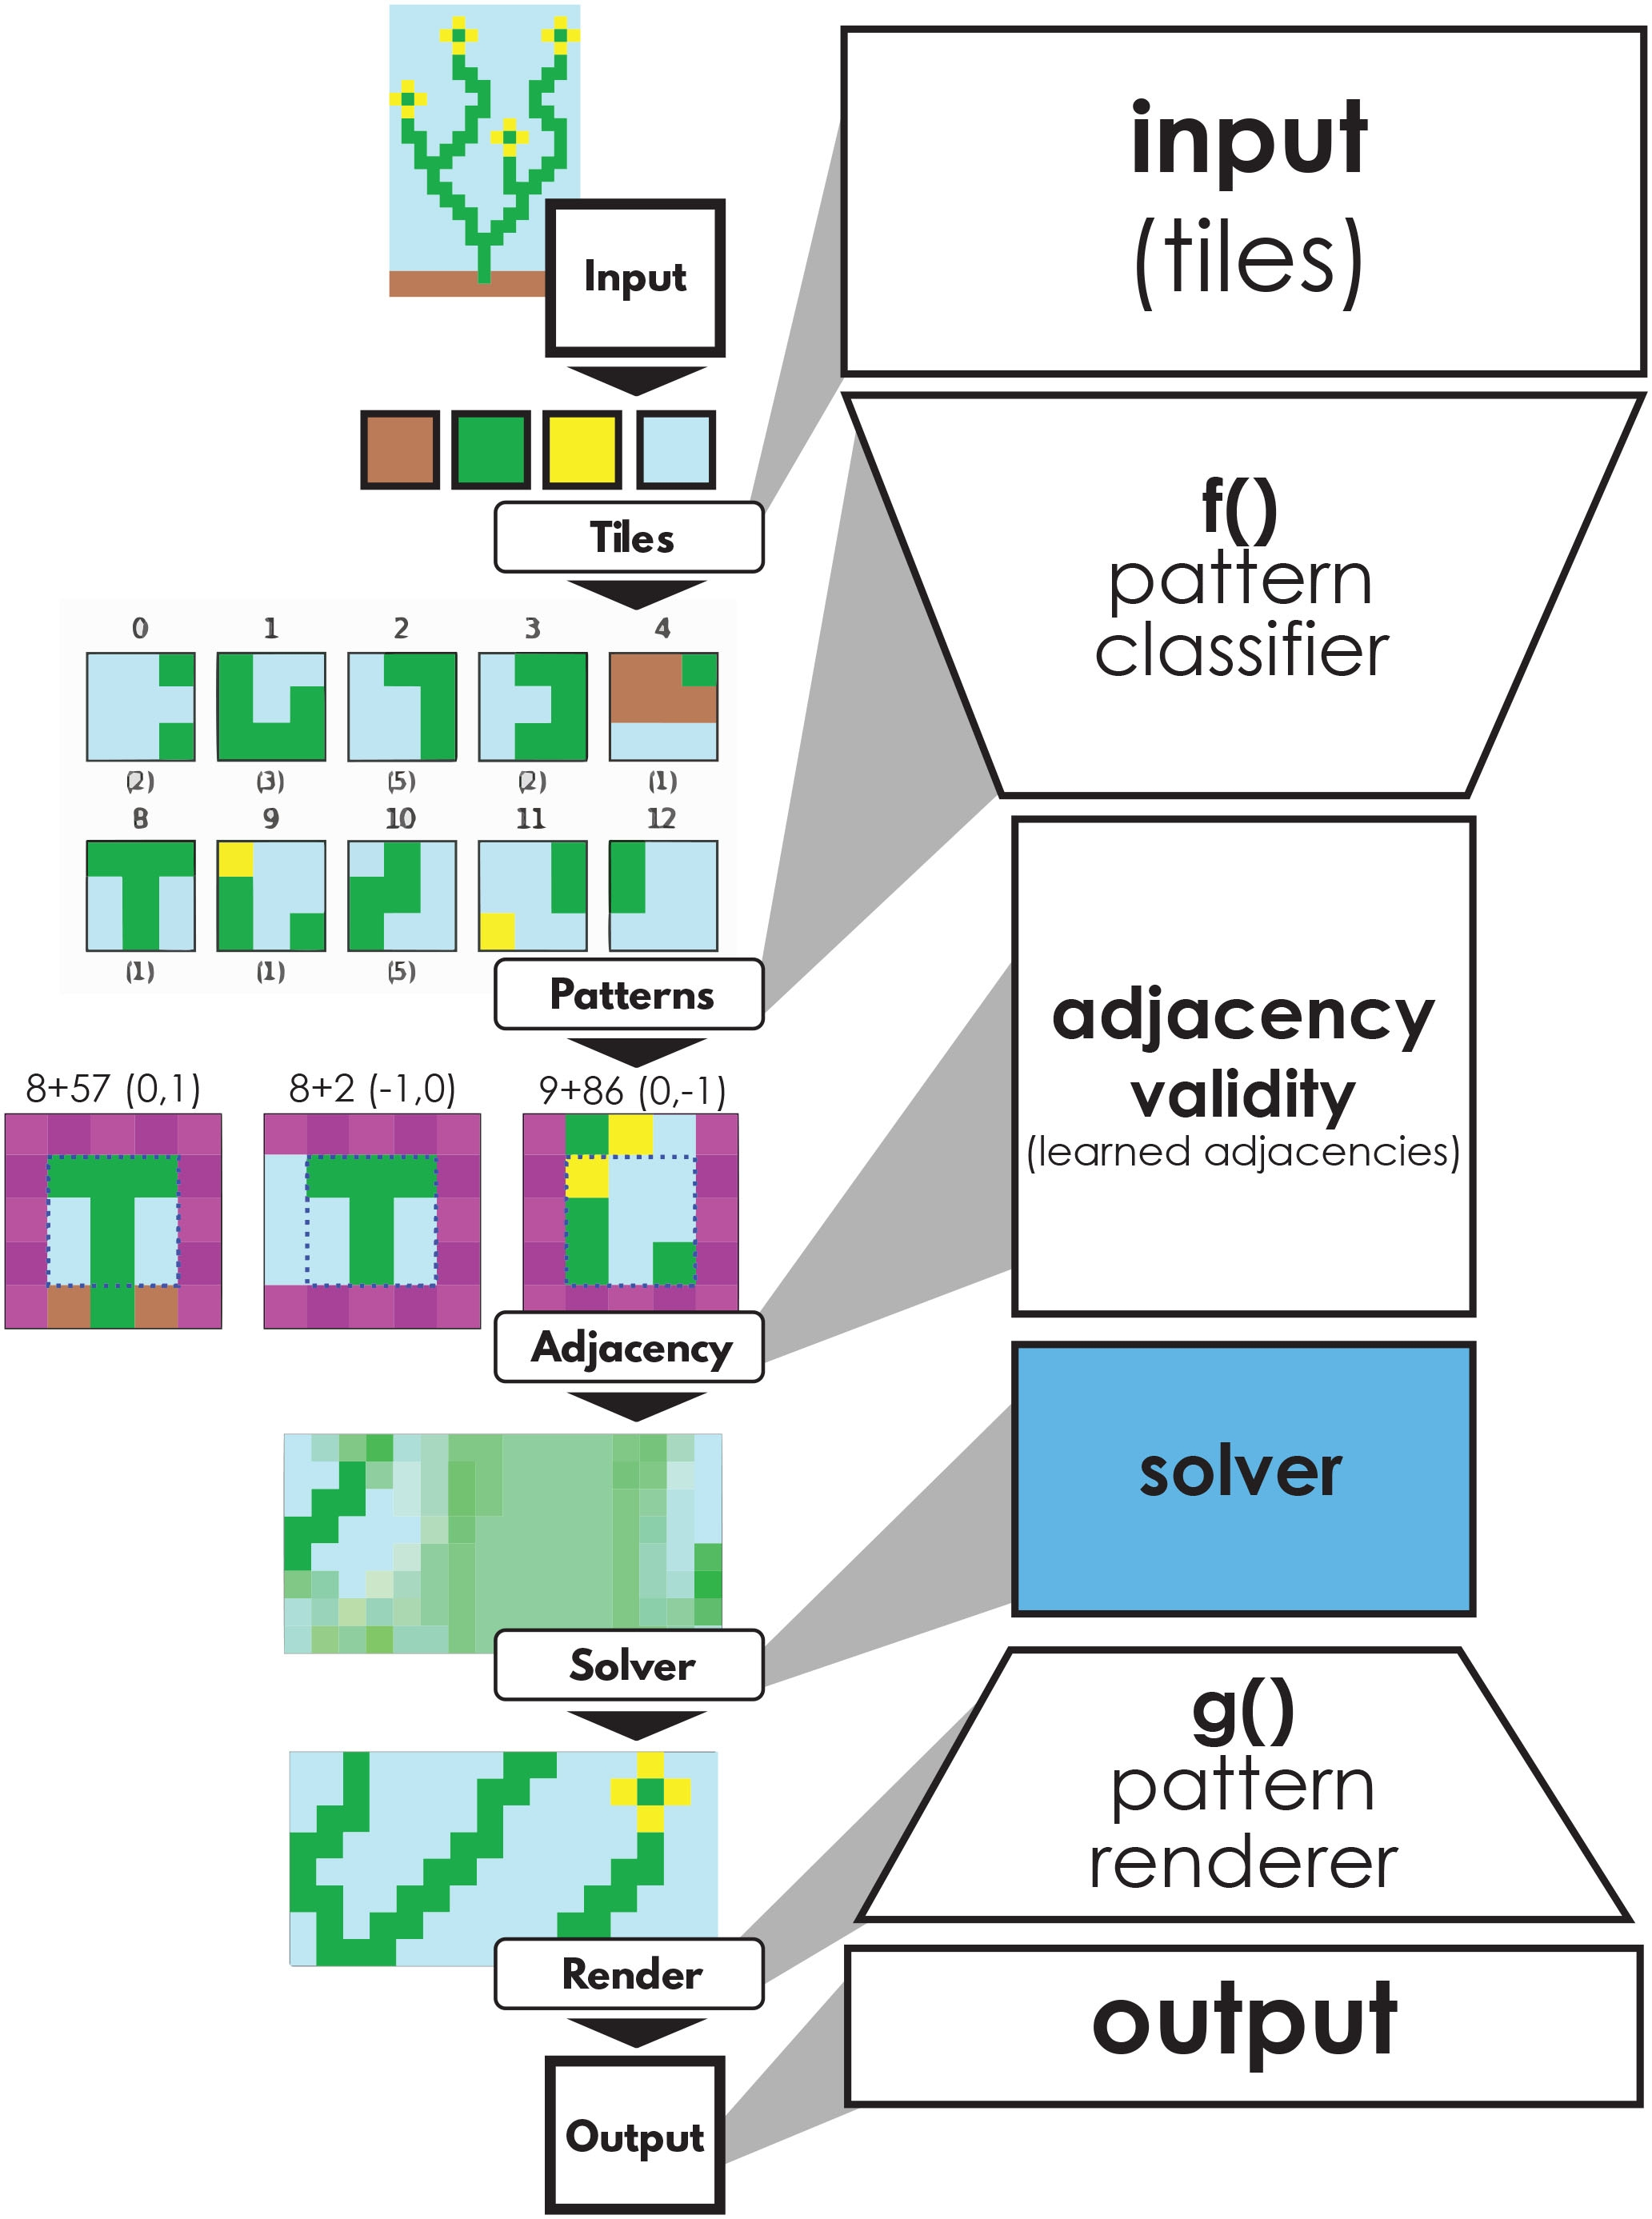
\includegraphics[width=\textwidth, height=0.5\textheight, keepaspectratio]{Images/OverlappingWFC.jpg}
    \caption{The overlapping \acrshort{wfc} pipeline with \(3\times 3\) overlap \cite{WFC_ConstraintSolving_and_ML}}
    \label{fig:overlappingWFC}
\end{figure}

\subsubsection{2D vs 3D}
While a lot of implementations focus solely on 2D input tiles and grids, fewer implementations support 3D input or output. This makes it a challenge to apply \acrshort{wfc} to 3D environments. Furthermore, the increased complexity from a 3D environment can lead to an increased failure rate, which requires techniques such as backtracking or modifying in blocks to counteract. This was highlighted in Figure \ref{fig:escheresque}.

\subsection{Limitations of WFC}
Research papers on \acrshort{wfc} frequently attempt to identify and find solutions for problems that implementations of the algorithm commonly face. Some of the most common problems are a lack of global constraints, overfitting and performance. These problems, as well as some other challenges, are discussed below.

%\begin{itemize}
%\item Isotropy / Homogeneity: Without global constraints there is no inherent overall structure.
%\item Overfitting: Adding too much detail to input or using too high overlapping can result in the input being copied directly too much.
%\item Performance: Slower than model synthesis [17]? Is this due to additional checks like lowest entropy vs scanning?
%\item Contradictions / Failures: Has a tendency to fail for big inputs, especially in 3D.
%\end{itemize}

\subsubsection{Lack of Global Constraints}\label{sec:lackOfGlobalConstraints}
One problem with \acrshort{wfc} is that, while output can be tailored to satisfy local constraints, global constraints are not inherently supported. This results in there being no inherent overall structure to the output. In other words, the output can be homogeneous.

In some applications, such as the game \textit{Caves of Qud} \cite{cavesofqud}, \acrshort{wfc} is used only after other algorithms have defined distinct regions of the map (Figure \ref{fig:cavesOfQudWFCHomogeneity}) \cite{WFC_ConstraintSolving_and_ML, WFC_Design_Constraints, GDC_caves_of_qud}. This multi-pass approach allows \acrshort{wfc} to be used to its strengths.

\begin{figure}[H]
    \centering
    \subfigure[Areas of the level set before using \acrshort{wfc}]{
        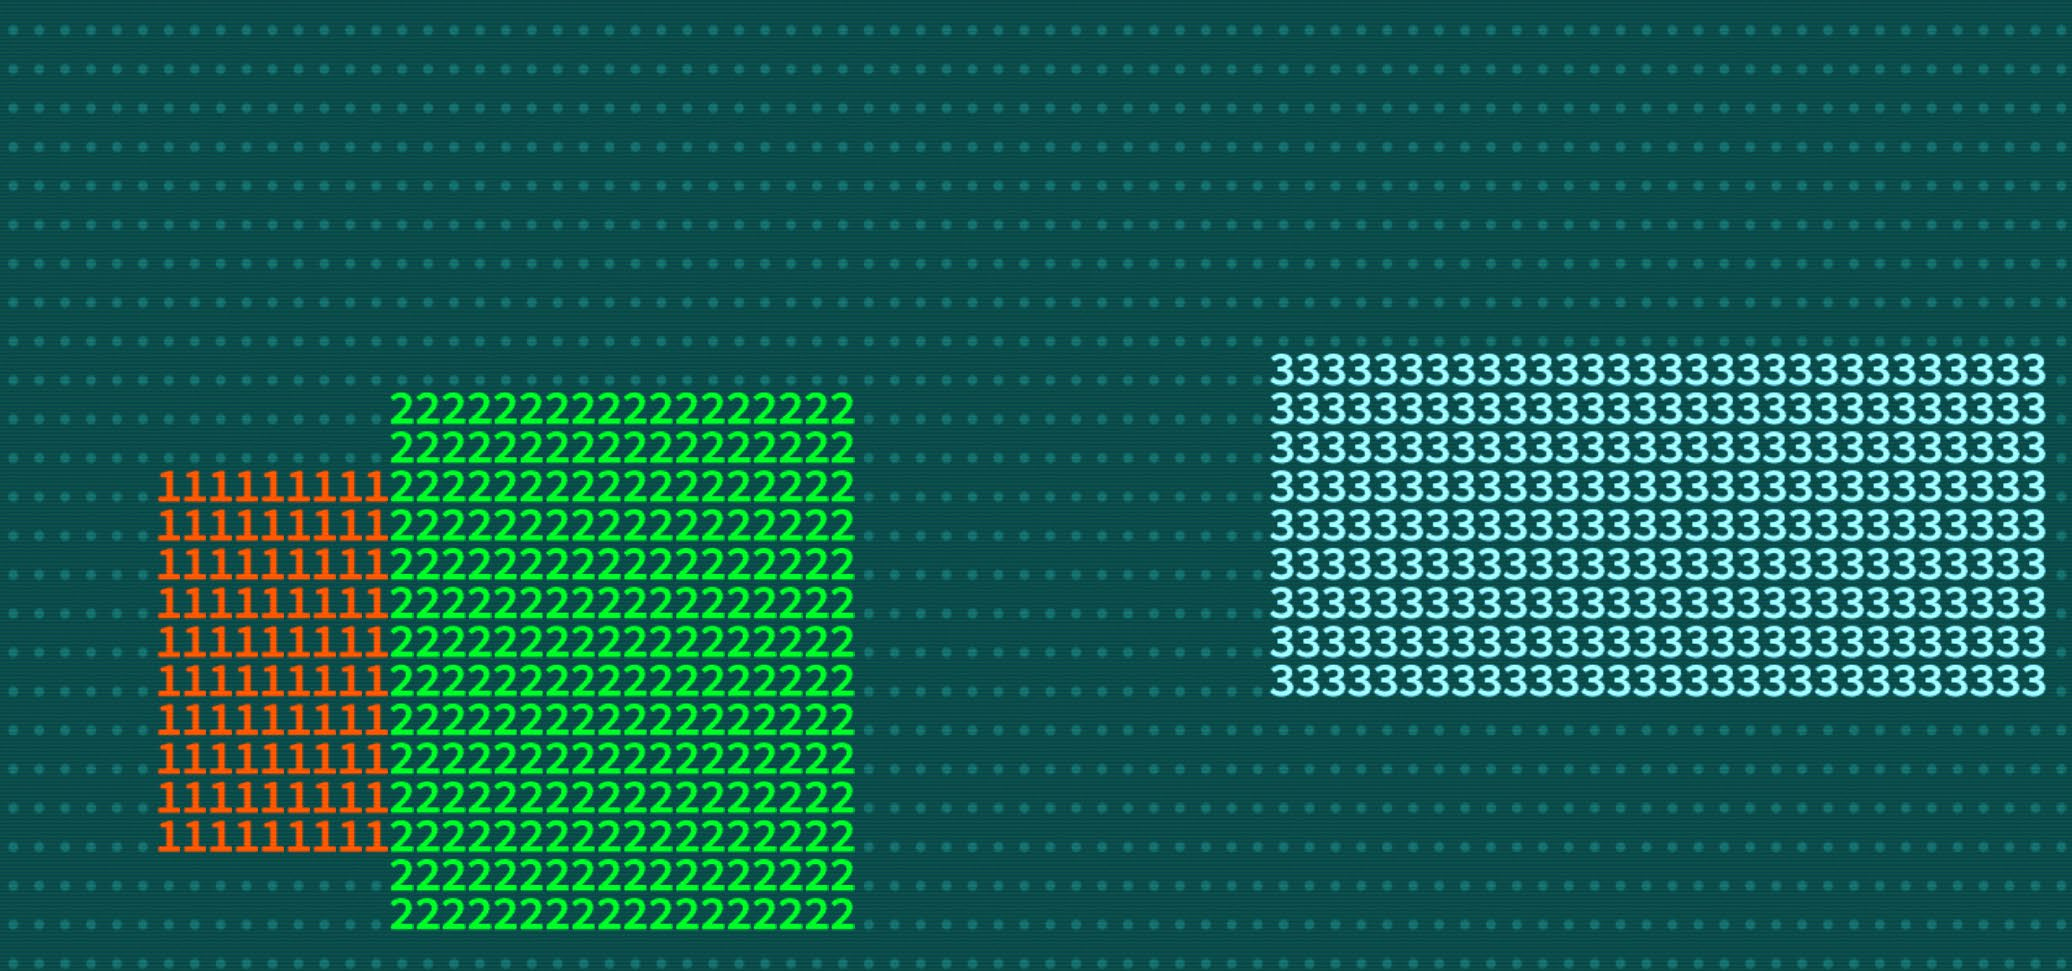
\includegraphics[width=0.475\textwidth, height=0.35\textheight, keepaspectratio]{Images/CavesOfQudWFC1.jpg}
        \label{fig:cavesOfQudWFC1}
    }
    \hfill
    \subfigure[Interiors generated using \acrshort{wfc}]{
        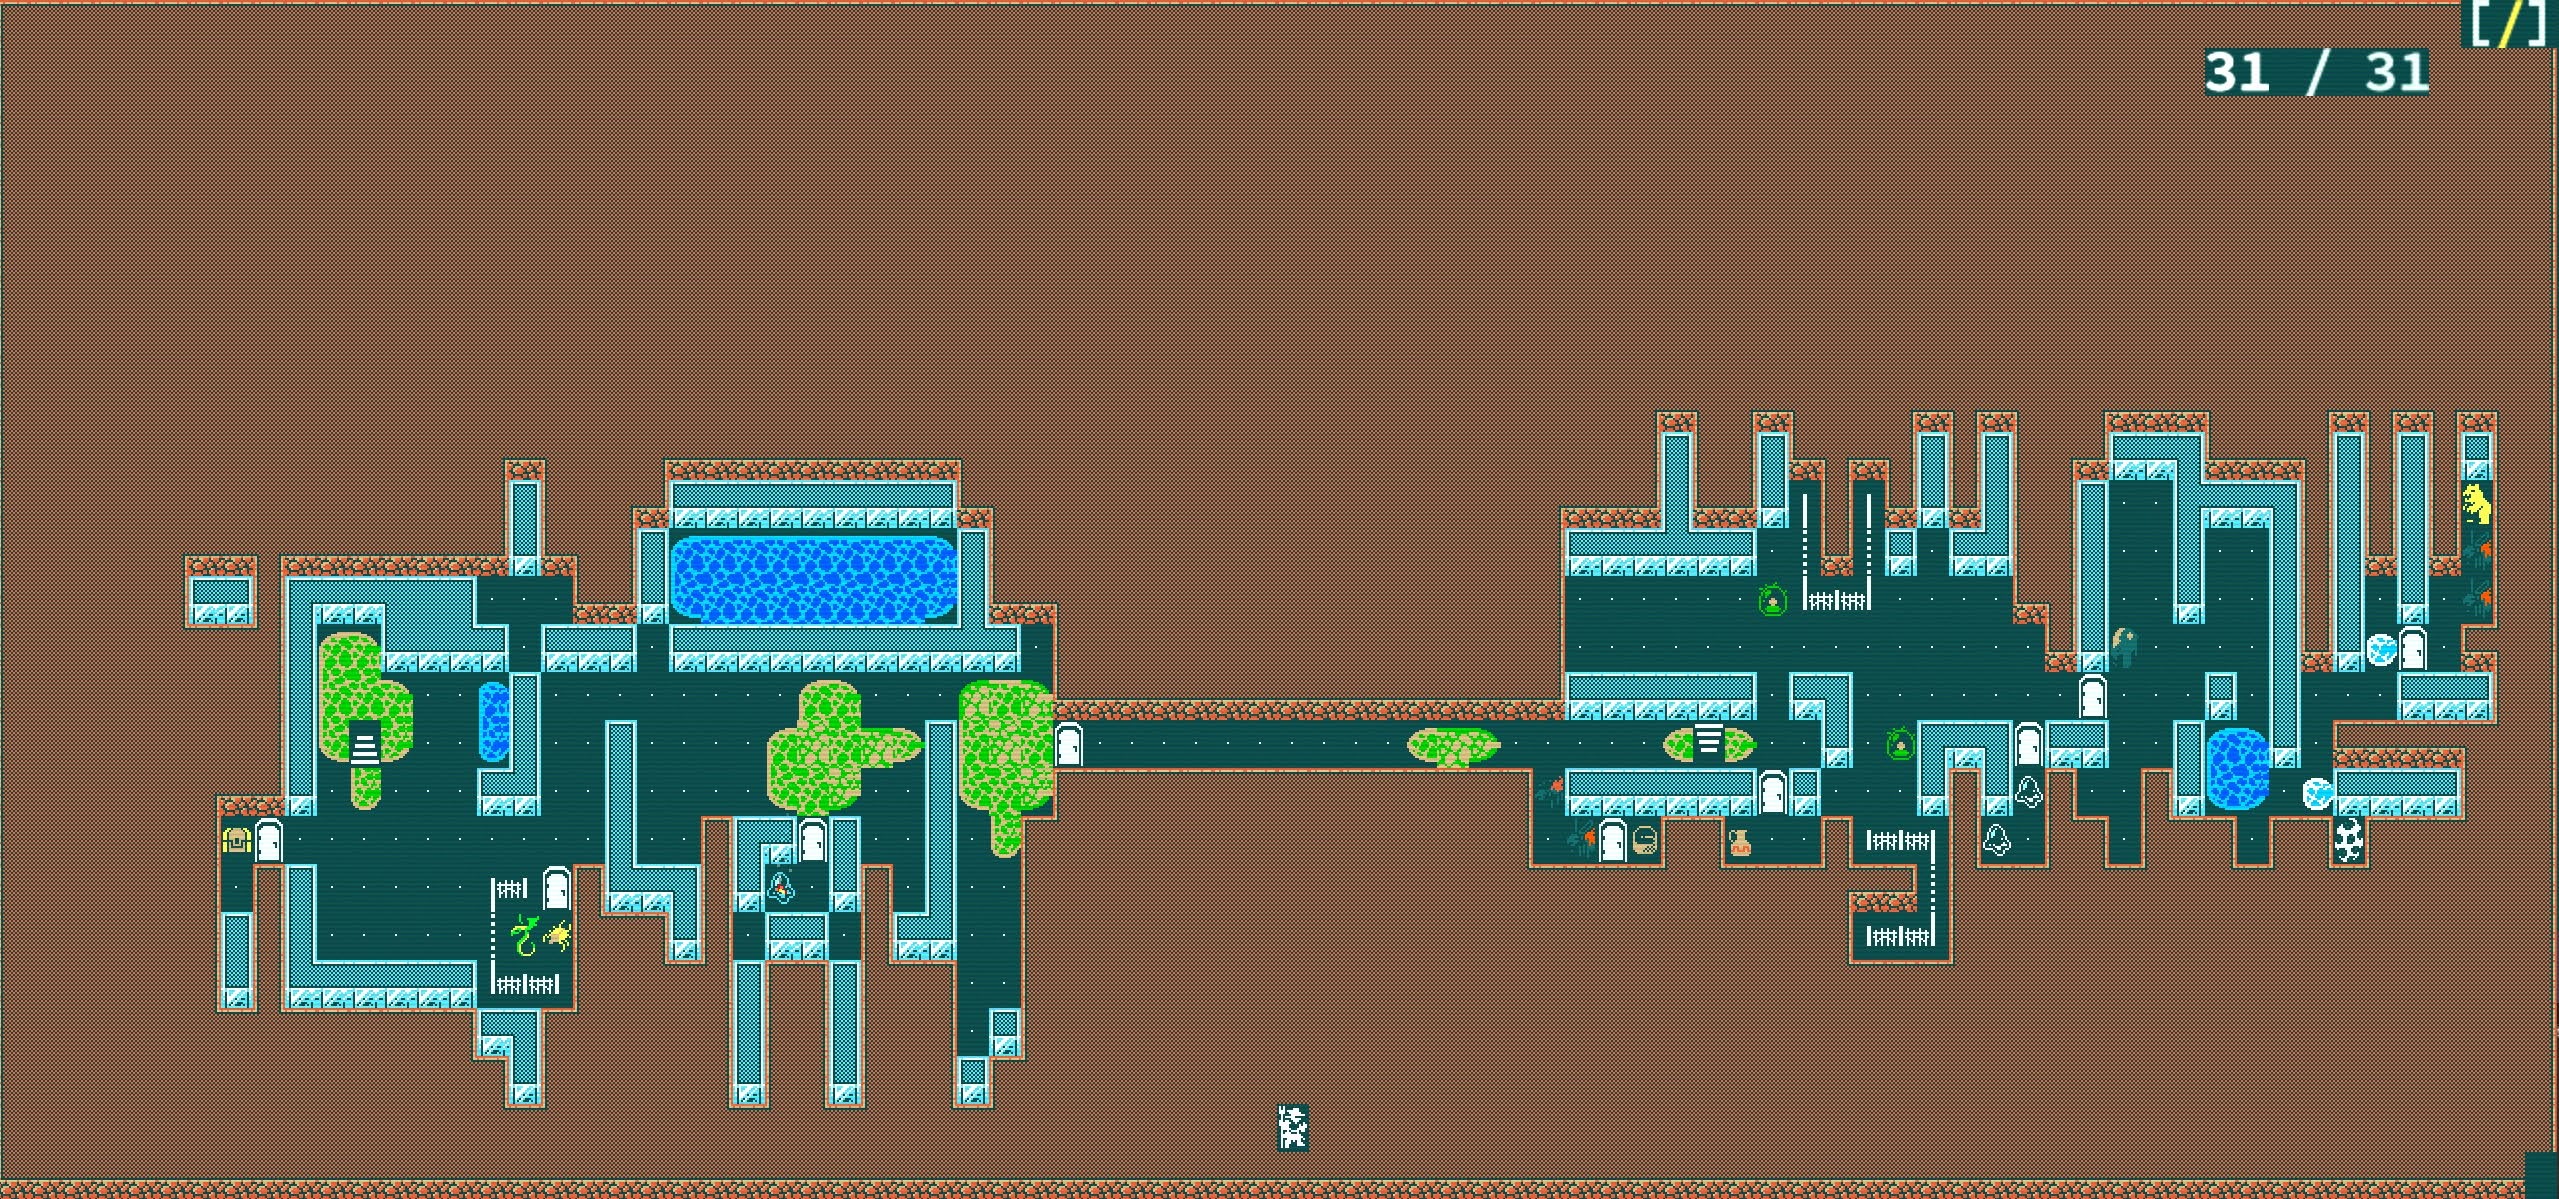
\includegraphics[width=0.475\textwidth, height=0.35\textheight, keepaspectratio]{Images/CavesOfQudWFC2.jpg}
        \label{fig:cavesOfQudWFC2}
    }
    \caption{\textit{Caves of Qud}'s multi-pass approach to avoid homogeneity \cite{GDC_caves_of_qud}}
    \label{fig:cavesOfQudWFCHomogeneity}
\end{figure}

To tackle the lack of global constraints, D. Cheng et al. add constraints on minimum tile count, maximum tile count and object distance \cite{WFC_Automatic_Rules_And_Better_Symmetries}. These are checked after each observation step.

The global maximum tile count constraint allows balancing of tile counts. This constraint is analogous to the use of weighted tile selection. Figure \ref{fig:wfcMaximumConstraint} shows the global maximum tile count constraint being used to reduce the amount of water in the level to match the desired design.

\begin{figure}[H]
    \centering
    \subfigure[Generation without the maximum constraint]{
        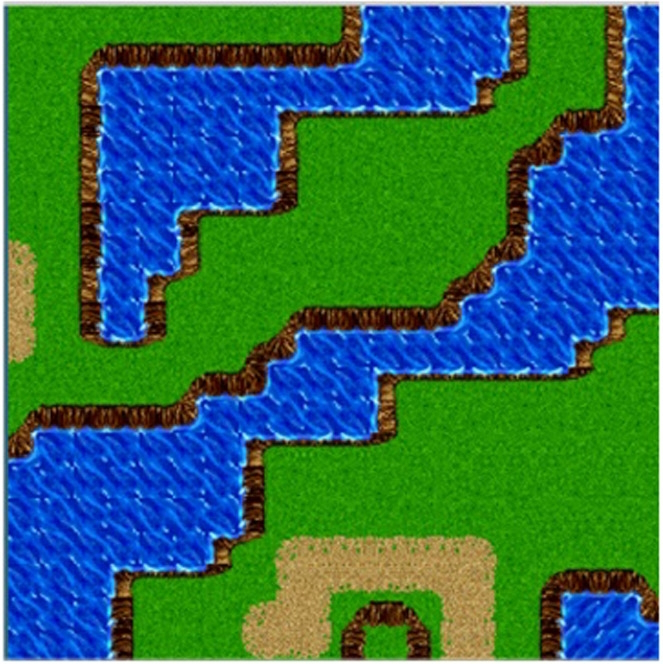
\includegraphics[width=0.475\textwidth, height=0.35\textheight, keepaspectratio]{Images/WFCMaximumConstraint1.jpg}
        \label{fig:wfcMaximumConstraint1}
    }
    \hfill
    \subfigure[Generation with the maximum constraint]{
        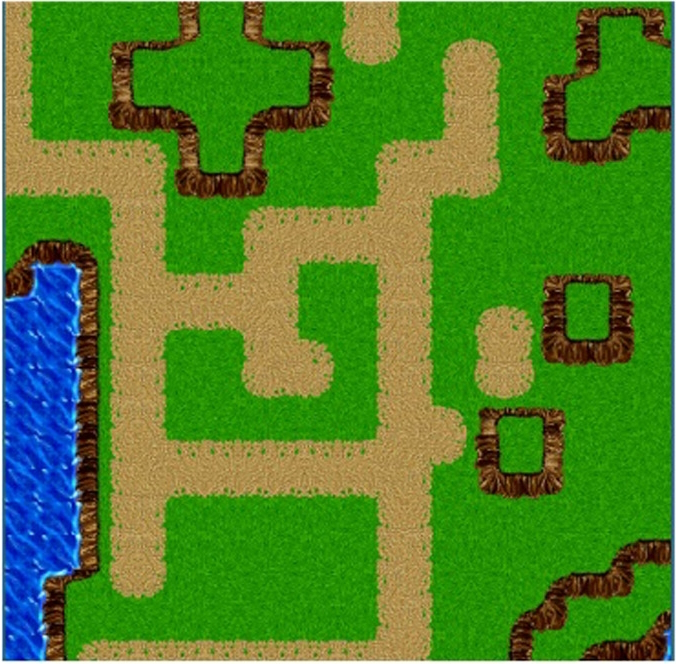
\includegraphics[width=0.475\textwidth, height=0.35\textheight, keepaspectratio]{Images/WFCMaximumConstraint2.jpg}
        \label{fig:wfcMaximumConstraint2}
    }
    \caption{Use of the global maximum constraint to limit water tiles \cite{WFC_Automatic_Rules_And_Better_Symmetries}}
    \label{fig:wfcMaximumConstraint}
\end{figure}

The global minimum tile count constraint gives more control on how tiles should be placed in the level. The way it is presented in the paper shows it being used to preset tiles before generation. This enables the definition of key areas that should be present in the output. Figure \ref{fig:wfcMinimumConstraint} shows the global minimum tile count constraint being used to place water in the bottom left and land in the middle of the level.

\begin{figure}[H]
    \centering
    \subfigure[Pre-setting water and land tiles]{
        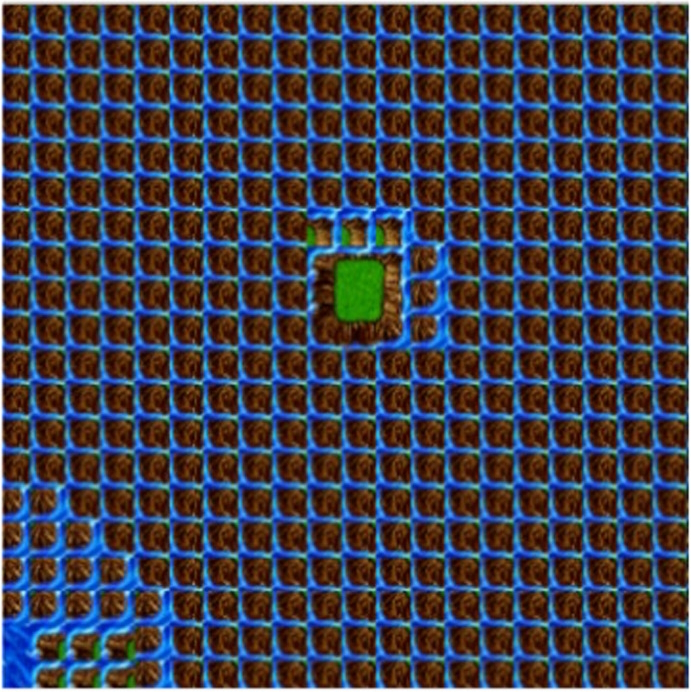
\includegraphics[width=0.475\textwidth, height=0.35\textheight, keepaspectratio]{Images/WFCMinimumConstraint1.jpg}
        \label{fig:wfcMinimumConstraint1}
    }
    \hfill
    \subfigure[Generation with the minimum constraint]{
        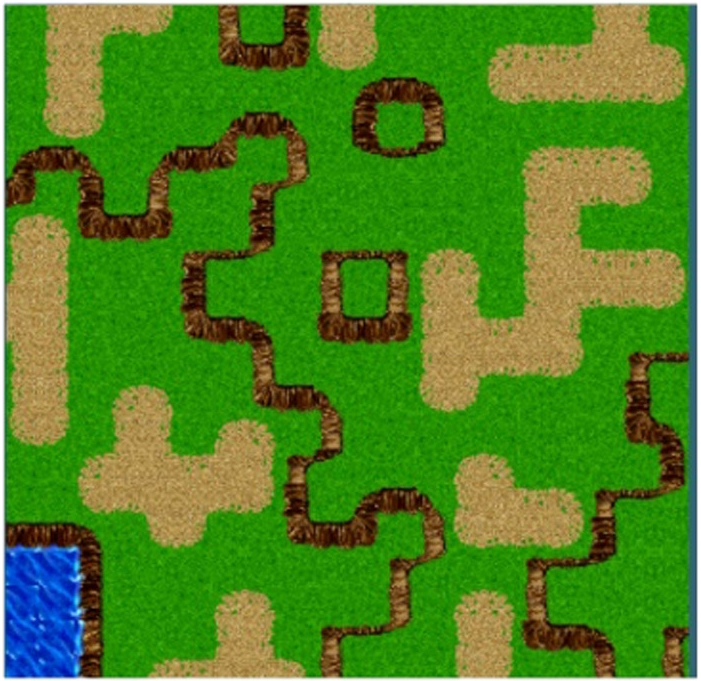
\includegraphics[width=0.475\textwidth, height=0.35\textheight, keepaspectratio]{Images/WFCMinimumConstraint2.jpg}
        \label{fig:wfcMinimumConstraint2}
    }
    \caption{Use of the global minimum constraint to pre-place tiles \cite{WFC_Automatic_Rules_And_Better_Symmetries}}
    \label{fig:wfcMinimumConstraint}
\end{figure}

The object distance constraint is used to create areas of interest, rather than scattering items equally throughout the level. Figure \ref{fig:wfcDistanceConstraint1} shows how, without an object distance constraint, enemies and items are scattered at random throughout the level. In contrast, Figure \ref{fig:wfcDistanceConstraint2} shows how enemies are clustered around a treasure chest. To achieve this, enemies are constrained to be fewer than 10 units away from chests. Furthermore, keys are constrained to be more than 10 units away from chests. This means that keys will not simply spawn next to chests, making finding them more interesting as the player must search the map.

\begin{figure}[H]
    \centering
    \subfigure[Generation without the distance constraint]{
        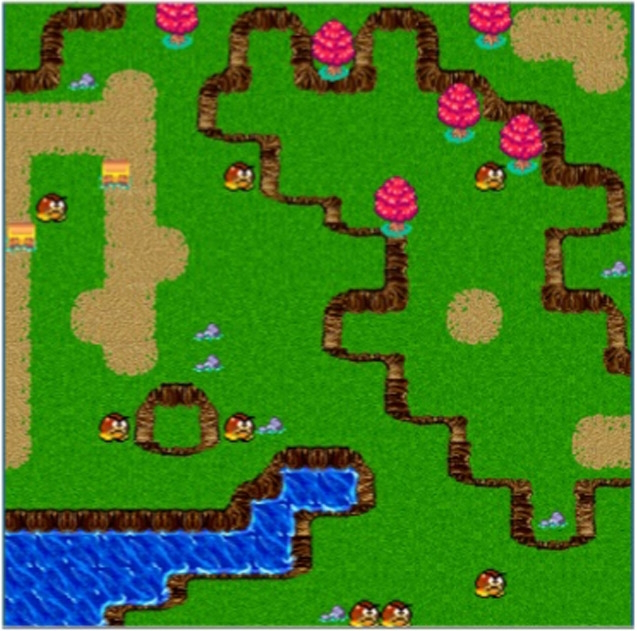
\includegraphics[width=0.475\textwidth, height=0.35\textheight, keepaspectratio]{Images/WFCDistanceConstraint1.jpg}
        \label{fig:wfcDistanceConstraint1}
    }
    \hfill
    \subfigure[Generation with the distance constraint]{
        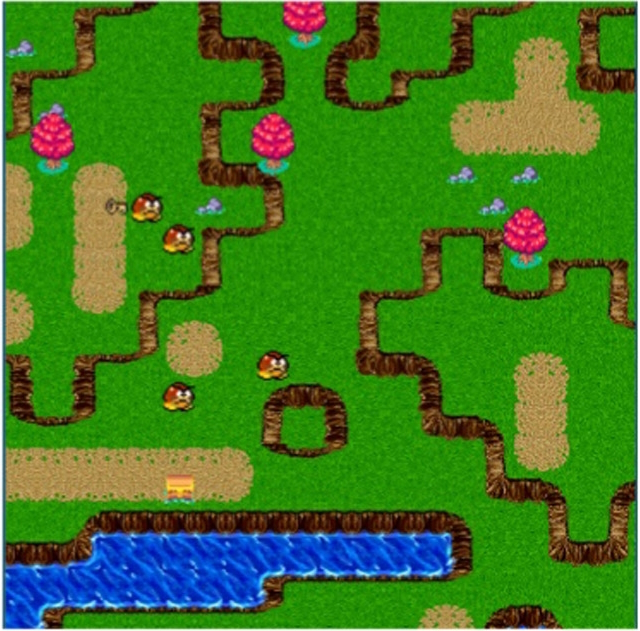
\includegraphics[width=0.475\textwidth, height=0.35\textheight, keepaspectratio]{Images/WFCDistanceConstraint2.jpg}
        \label{fig:wfcDistanceConstraint2}
    }
    \caption{Use of the object distance constraint to improve object spawns \cite{WFC_Automatic_Rules_And_Better_Symmetries}}
    \label{fig:wfcDistanceConstraint}
\end{figure}

One additional option included is to carry out generation in two passes. This helps create levels of certain styles and to reduce conflicts arising from trying to generate everything in one pass, such as placing an object on an unsuitable tile. In Figure \ref{fig:wfcMultiLayer}, double-layer generation is used to spawn enemies on grass and chests on dirt roads. Furthermore, rock and dirt decor is placed on suitable tiles.

\begin{figure}[H]
    \centering
    \subfigure[Single-layer generation]{
        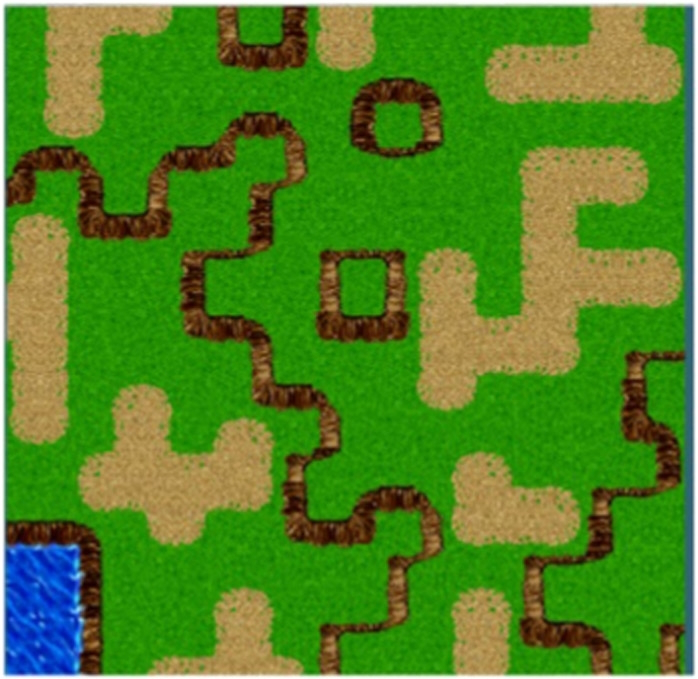
\includegraphics[width=0.475\textwidth, height=0.35\textheight, keepaspectratio]{Images/WFCMultiLayer1.jpg}
        \label{fig:wfcMultiLayer1}
    }
    \hfill
    \subfigure[Double-layer generation]{
        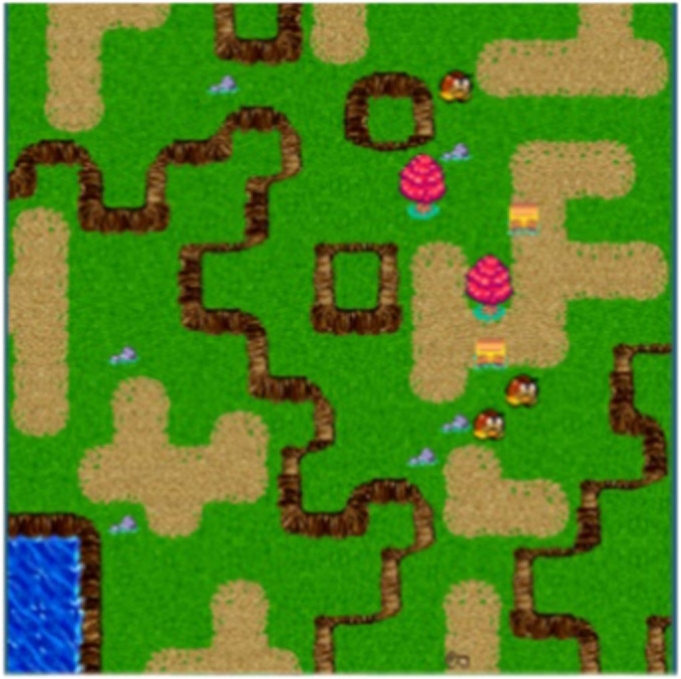
\includegraphics[width=0.475\textwidth, height=0.35\textheight, keepaspectratio]{Images/WFCMultiLayer2.jpg}
        \label{fig:wfcMultiLayer2}
    }
    \caption{Use of the double-layer generation to ease object spawning \cite{WFC_Automatic_Rules_And_Better_Symmetries}}
    \label{fig:wfcMultiLayer}
\end{figure}

A. Sandhu et al. achieve the same goal as minimum and maximum tile count constraints through the use of a weighted choice \cite{WFC_Design_Constraints}. In addition to using entropy to choose the most constrained tile after each propagation step, assigning a weight to each choice can encourage the algorithm to choose a different balance of tiles. Furthermore, the authors introduce a second observation step. This performs a second, smaller scale \acrshort{wfc} algorithm, which can be used to refine item placement and create subregions within a map.

Solutions altering \acrshort{wfc} directly to support global constraints are faced with the issue that the additional constraints can have a negative impact on performance. However, by combining such solutions with those discussed in the Performance Subsection (\ref{sec:performance}), the impact can be reduced \cite{WFC_ConstraintSolving_and_ML}.

\subsubsection{Overfitting}
When adding a lot of detail to the input, such as through using complex tile sets, the output may become too constrained. This can result in overfitting and an increased failure rate.

One solution is to use a multi-pass approach. This not only reduces the risk of overfitting, but also helps to globally constrain the output. This is done by reducing the detail of the input and instead adding additional details to the output in a second pass once \acrshort{wfc} has run. \textit{Caves of Qud} applies this approach by generating architecture using \acrshort{wfc} and then generating details using additional passes (Figure \ref{fig:cavesOfQudWFCOverfitting}) \cite{GDC_caves_of_qud}.

\begin{figure}[H]
    \centering
    \subfigure[Architecture generated using \acrshort{wfc}]{
        
\includegraphics[width=0.475\textwidth, height=0.35\textheight, keepaspectratio]{Images/CavesOfQudWFC3.jpg}
        \label{fig:cavesOfQudWFC3}
    }
    \hfill
    \subfigure[Details filled using additional passes]{
        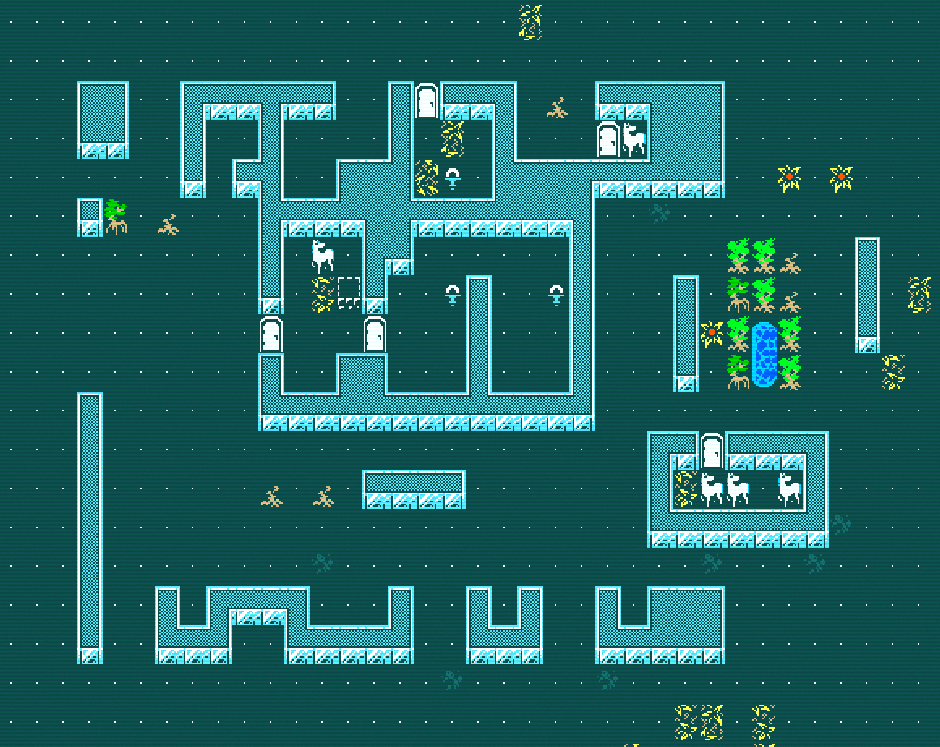
\includegraphics[width=0.475\textwidth, height=0.35\textheight, keepaspectratio]{Images/CavesOfQudWFC4.png}
        \label{fig:cavesOfQudWFC4}
    }
    \caption{\textit{Caves of Qud}'s multi-pass approach to avoid overfitting \cite{GDC_caves_of_qud}}
    \label{fig:cavesOfQudWFCOverfitting}
\end{figure}

%Furthermore, when using the overlapping method for WFC, a high overlap parameter will also result in overfitting. This may be difficult to balance depending on the input.

\subsubsection{Performance}\label{sec:performance}
Another issue identified with \acrshort{wfc} is performance. While the chance of success is high with small inputs, larger inputs are much likelier to fail, especially with more complicated tile sets \cite{WFC_ConstraintSolving_and_ML}. This can result in a significant generation time for large output grids as generation must be restarted several times. Several solutions to \acrshort{wfc}'s scalability problem have been proposed.%(More citations and graph of performance)

One of the most common solutions is to include some form of backtracking, which allows further searching of the search space upon a contradiction instead of having to restart. However, with complex tile sets, care must be taken to reduce the chance of backtracking exploring an unpromising search space for an extended time as in the 3D Escheresque example shown previously in Figure \ref{fig:escheresque}. Using a search heuristic could help with this. I. Karth and A. M. Smith compared the performance of \acrshort{wfc} with and without backtracking and global constraints, finding that backtracking is critical to improving performance when using global constraints (Figure \ref{fig:backtrackingPerformance}) \cite{WFC_ConstraintSolving_and_ML}.

\begin{figure}[H]
    \centering
    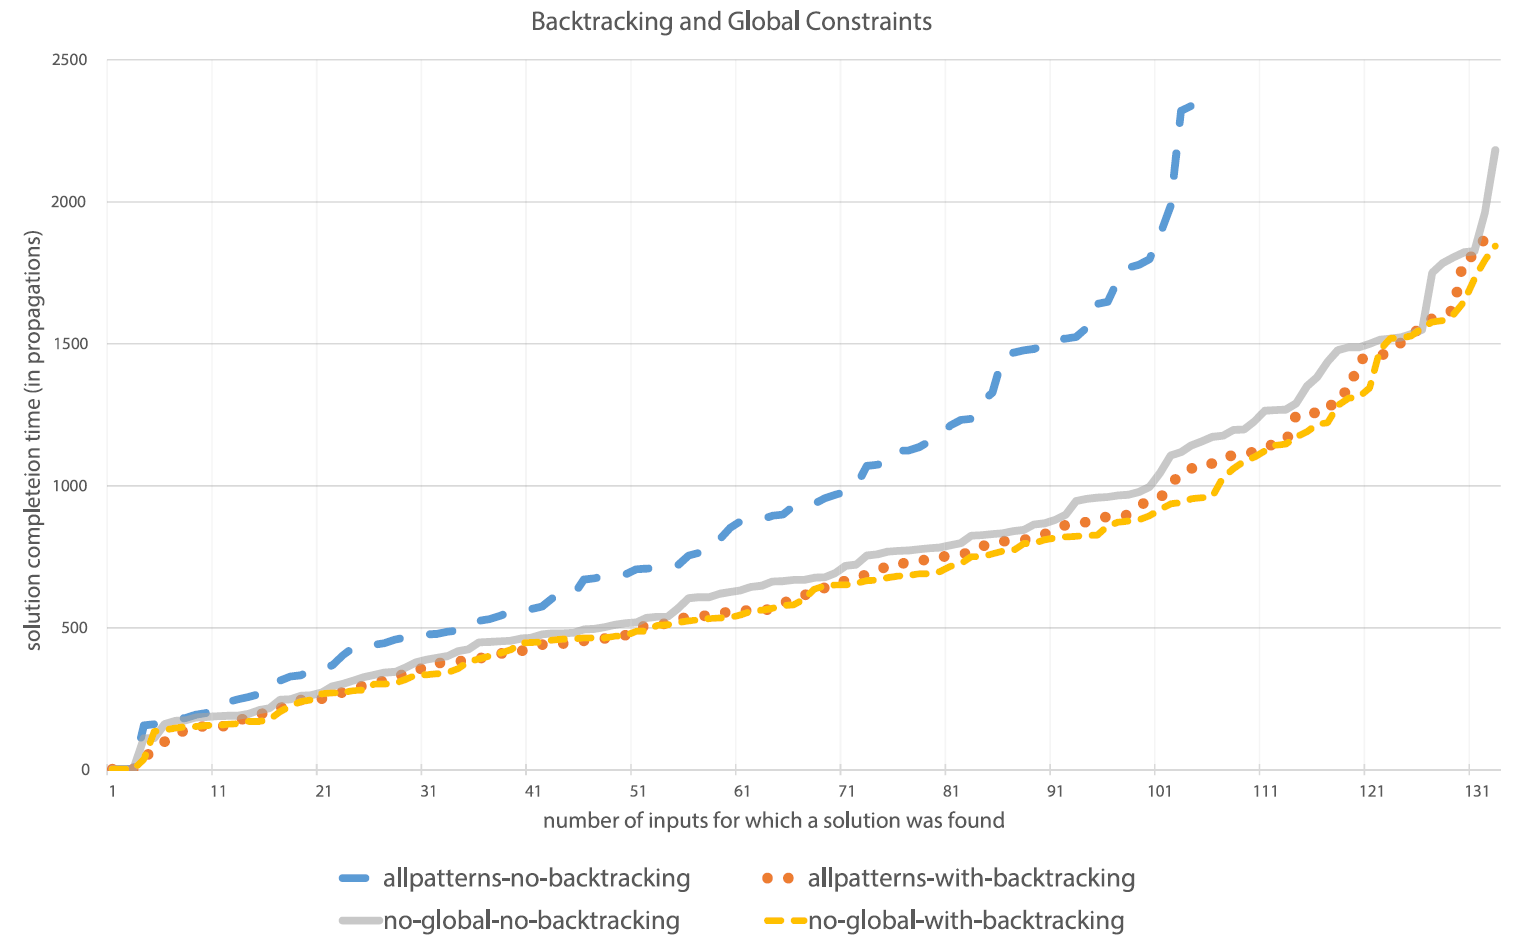
\includegraphics[width=\textwidth, height=0.3\textheight, keepaspectratio]{Images/BacktrackingPerformance.png}
    \caption{Comparing performance of \acrshort{wfc} with and without backtracking and global constraints. When using global constraints, backtracking significantly improves performance. \cite{WFC_ConstraintSolving_and_ML}}
    \label{fig:backtrackingPerformance}
\end{figure}

Nested \acrshort{wfc} (N-WFC) \cite{Nested_WFC} is one technique that aims to improve scalability of \acrshort{wfc}. It splits a larger grid into smaller grids, evaluating sub-grids diagonally from the top left (Figure \ref{fig:nestedWFC}). Each sub-grid overlaps constraints from its left and upper neighbour to satisfy constraints between adjacent sub-grids. This can be extended to an infinite space by overlapping new areas with old areas (Figure \ref{fig:infiniteWFC}). While this technique does improve the performance of \acrshort{wfc}, a large number of conflicts from edge data still occur.

\begin{figure}[H]
    \centering
    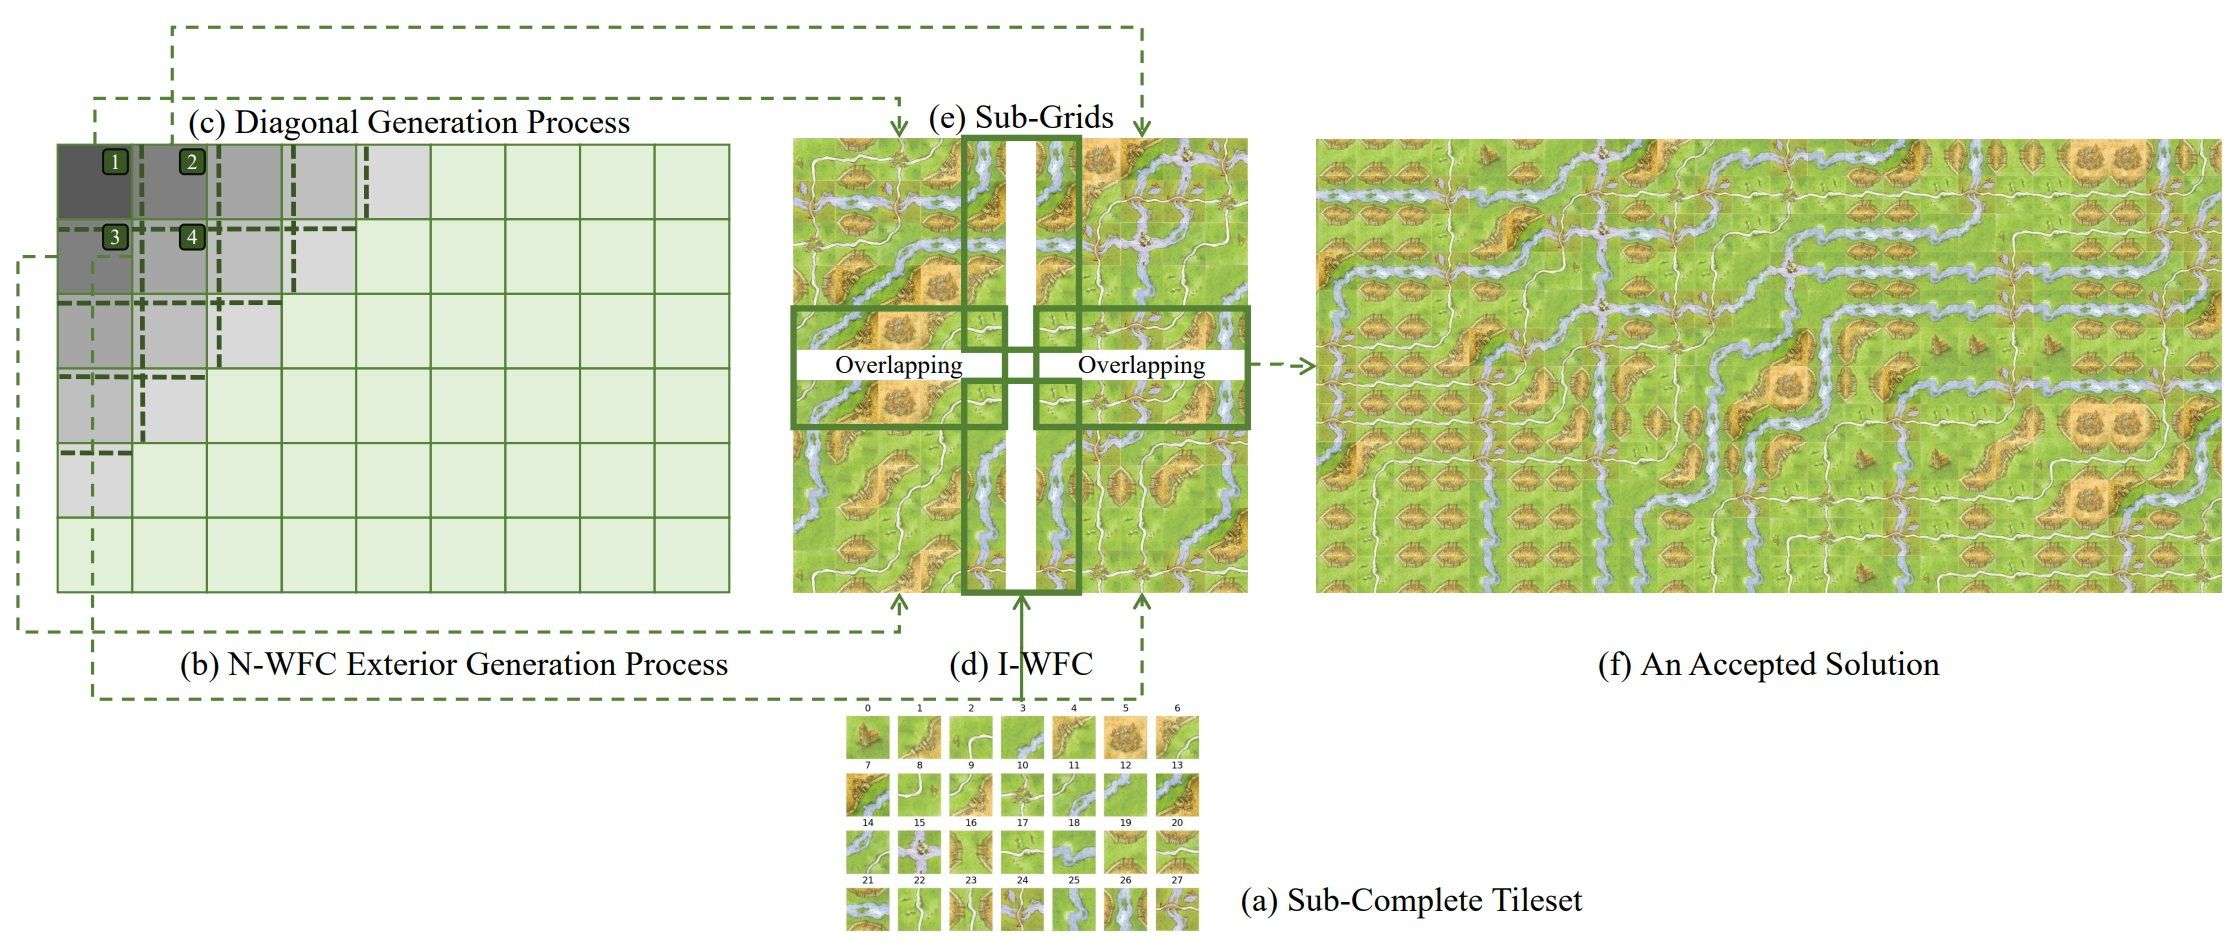
\includegraphics[width=\textwidth, height=0.3\textheight, keepaspectratio]{Images/NestedWFC.jpg}
    \caption{Large-scale game implementation with N-WFC and sub-complete tile set. First, it requires (a) one sub-complete tile set. Then the (b) Exterior Generation Process uses (c) Diagonal Generation Process to start generating. Each (d) sub-grid uses (e) I-WFC to find an accepted solution and overlap its edge with the adjacent sub-grids, forming an (f) final soluton. \cite{Nested_WFC}}
    \label{fig:nestedWFC}
\end{figure}

\begin{figure}[H]
    \centering
    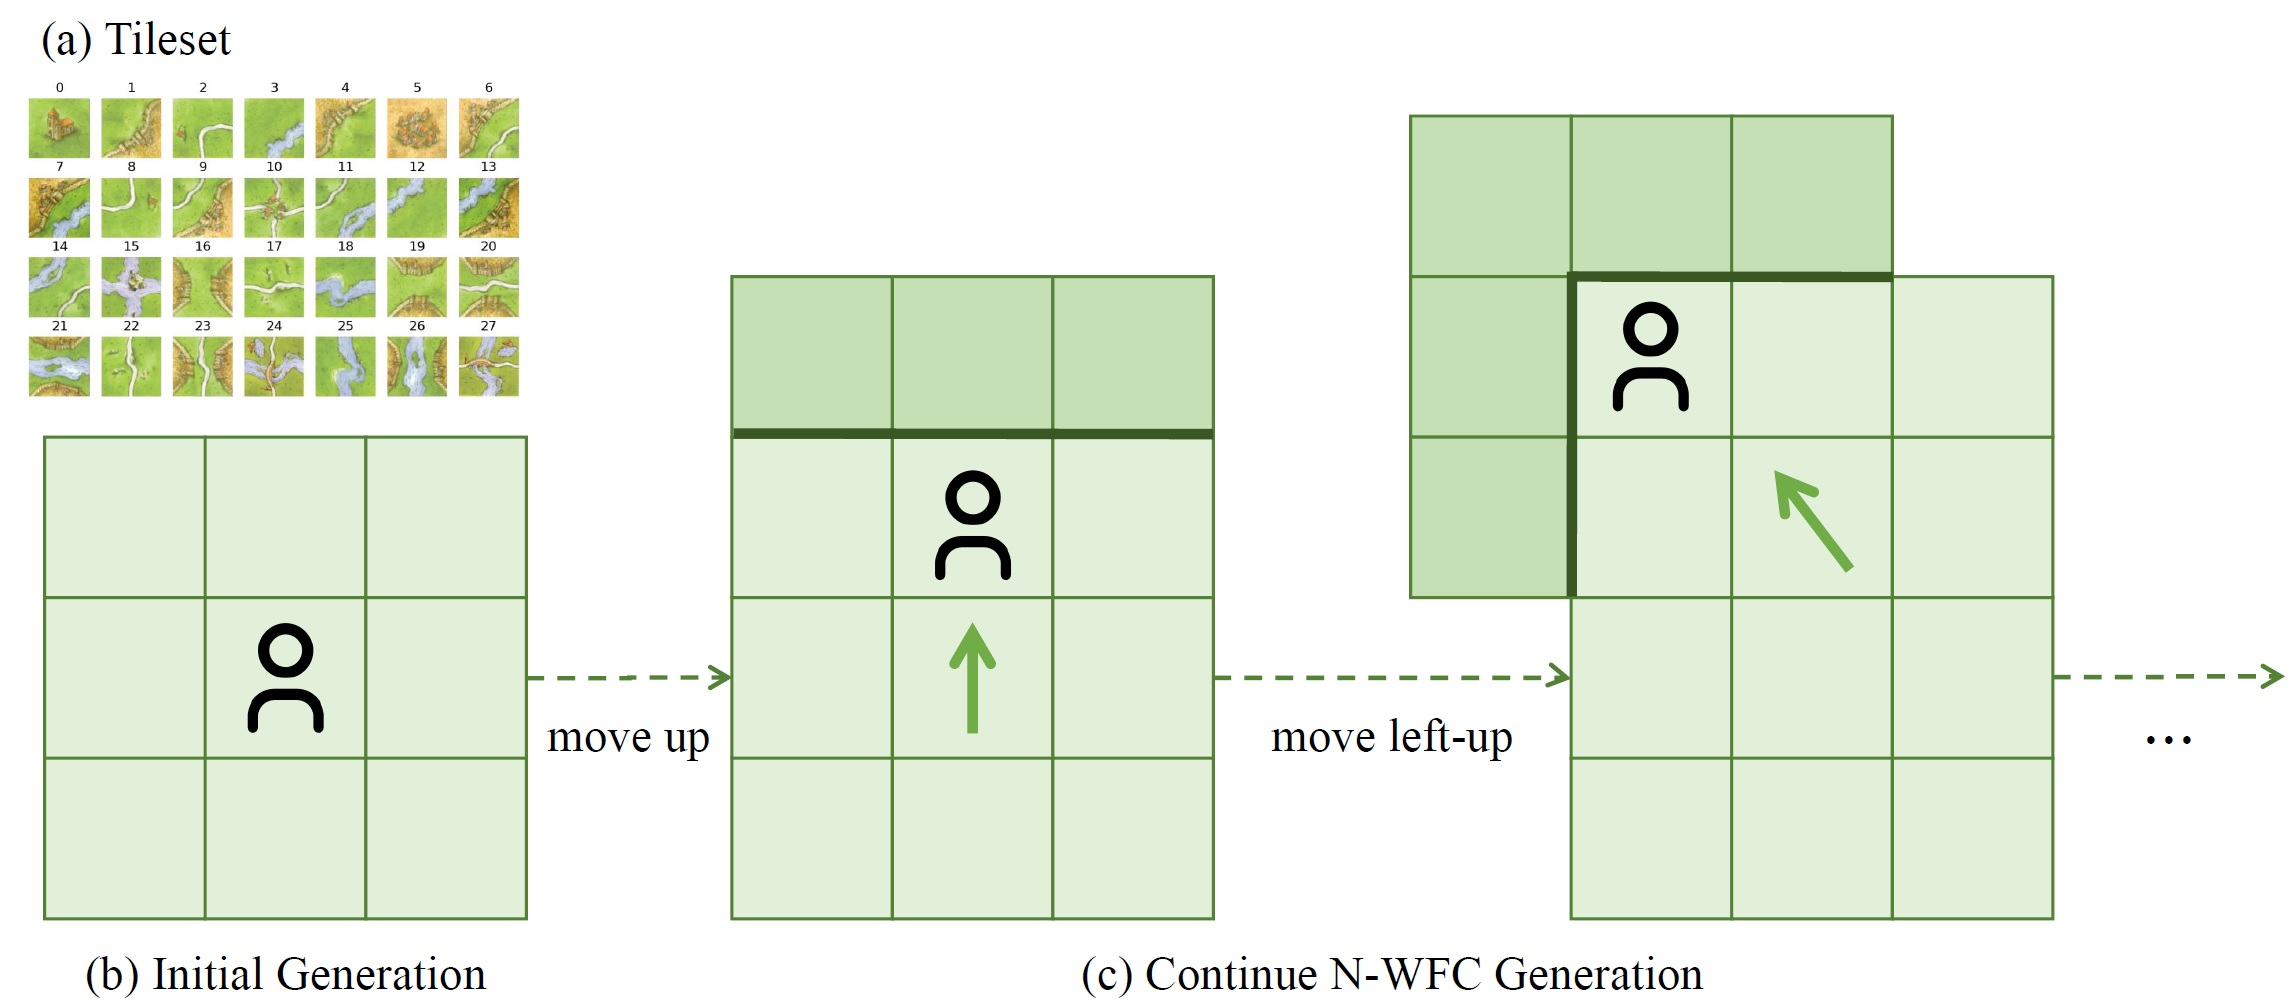
\includegraphics[width=\textwidth, height=0.3\textheight, keepaspectratio]{Images/InfiniteWFC.jpg}
    \caption{Infinite game implementation with N-WFC and sub-complete tile set \cite{Nested_WFC}}
    \label{fig:infiniteWFC}
\end{figure}

Another technique, \acrlong{imib} \cite{Infinite_Modifying_In_Blocks}, applies \acrshort{wfc} multiple times in small chunks. Keeping the chunks small keeps the performance of generation high, while running \acrshort{wfc} in four layers per chunk ensures that constraints are satisfied between adjacent chunks. The layering also addresses the limitation of conflicts that Nested \acrshort{wfc} struggles with. As each chunk is made up of four \acrshort{wfc} layers, failed layers can usually be ignored rather than having to be regenerated. However, this comes with computational overhead from running \acrshort{wfc} four times per chunk. An overview of the method is shown in Figure \ref{fig:imib}, with detailed discussion in Section \ref{sec:IMIB}.

% IMIB FIGURE
\begin{figure}[H]
    \centering
    \subfigure[After layer 1 has been generated]{
        
\includegraphics[width=0.475\textwidth, height=0.35\textheight, keepaspectratio]{Images/IMIB3.png}
        \label{fig:imib3}
    }
    \hfill
    \subfigure[Preparing layer 2 with overlap into layer 1]{
        
\includegraphics[width=0.475\textwidth, height=0.35\textheight, keepaspectratio]{Images/IMIB4.png}
        \label{fig:imib4}
    }

    \vspace{\baselineskip} % add some vertical space between the rows

    \subfigure[After layers 1 and 2 have been generated]{
        
\includegraphics[width=0.475\textwidth, height=0.35\textheight, keepaspectratio]{Images/IMIB5.png}
        \label{fig:imib5}
    }
    \hfill
    \subfigure[After all layers have been generated]{
        
\includegraphics[width=0.475\textwidth, height=0.35\textheight, keepaspectratio]{Images/IMIB9.png}
        \label{fig:imib9}
    }
    \caption{A glimpse into the \acrshort{imib} pipeline. Each layer defines a small part of each chunk to run \acrshort{wfc} in. By clearing and running four overlapping layers, a full grid is generated. \cite{Infinite_Modifying_In_Blocks}}
    \label{fig:imib}
\end{figure}

\subsubsection{Other Challenges}
Environments of a certain style, especially those trying to create a realistic feel, may struggle from \acrshort{wfc}'s use of a grid structure for its output. However, if this regular grid is transformed into an irregular quadrilateral grid, more complex shapes can be used. H. Kim et al. achieve this by using a graph-based data structure, which can be integrated with a navigation mesh in 3D as shown in Figure \ref{fig:navigationMeshNodePlacement} \cite{WFC_Graph-based}. However, this solution is limited due to a lack of control over solution order.

\begin{figure}[H]
    \centering
    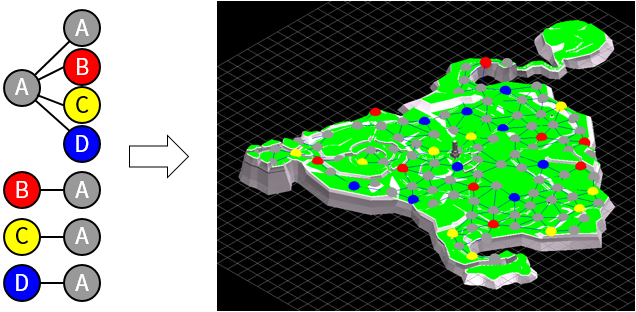
\includegraphics[width=\textwidth, height=0.3\textheight, keepaspectratio]{Images/NavigationMeshNodePlacement.png}
    \caption{Placing nodes on a navigation mesh using graph-based \acrshort{wfc} \cite{WFC_Graph-based}}
    \label{fig:navigationMeshNodePlacement}
\end{figure}

Taking the idea of irregular quadrilateral grids further, T. Møller and J. Billeskov explore the use of a growing grid neural network to augment \acrshort{wfc} \cite{WFC_Neural_Network}. Growing grid can be used to create irregular quadrilateral grids that fit a given input shape (Figure \ref{fig:growingGrid1}). Here, gradients can be used to control grid density. \acrshort{wfc} output can then be fit onto an irregular quadrilateral grid to create more interesting worlds (Figure \ref{fig:growingGrid2}). The authors also found that players have higher self-confidence in navigating irregularly-shaped maps and an increased ability to form mental maps of their environment.

\begin{figure}[H]
    \centering
    \subfigure[Growing grid creating an irregular quadrilateral grid fitting an input shape]{
        
\includegraphics[width=0.475\textwidth, height=0.35\textheight, keepaspectratio]{Images/GrowingGridShape.png}
        \label{fig:growingGrid1}
    }
    \hfill
    \subfigure[Fitting \acrshort{wfc} onto an irregular quadrilateral grid to create more complex worlds]{
        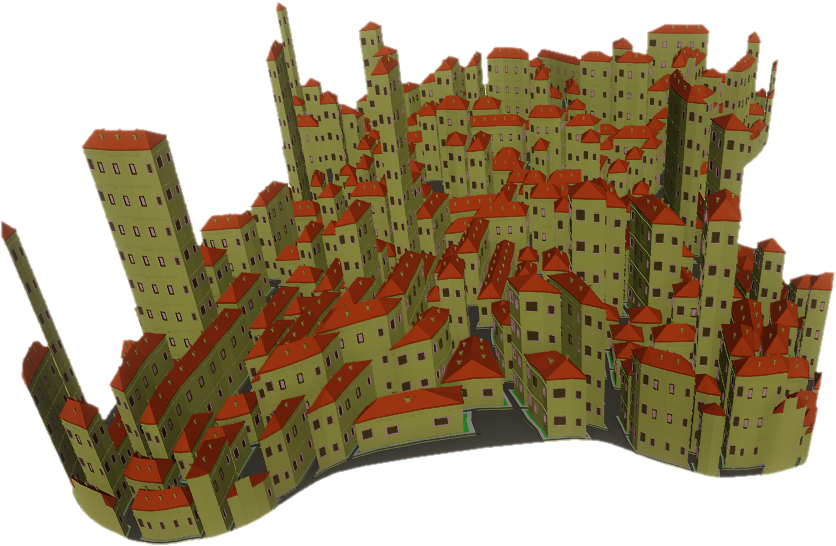
\includegraphics[width=0.475\textwidth, height=0.35\textheight, keepaspectratio]{Images/GrowingGridWFC.png}
        \label{fig:growingGrid2}
    }
    \caption{Using growing grid and \acrshort{wfc} to generate more complex worlds \cite{WFC_Neural_Network}}
    \label{fig:growingGrid}
\end{figure}

Very simple implementations may ignore symmetry when defining tile neighbours in the simple tiled method \cite{Easy_WFC}. Instead, every neighbour for each direction of each tile is listed explicitly. While this keeps the code simple, it means that a huge amount of work is required when defining neighbours for complex tile sets, with high chance of human error. The original \acrshort{wfc} implementation and several others define a symmetry type for each tile to tackle enumeration of large tile sets. This means that much less data about the input has to be provided, lessening the work required and chance of human error. The original \acrshort{wfc} implementation defines five symmetry types, which it applies to a variety of 2D images. D. Cheng et al. instead define nine symmetry types as in Table \ref{fig:symmetryDictionary}, which supports a greater variety of tile sets \cite{WFC_Automatic_Rules_And_Better_Symmetries}.

\begin{table}[H]
    \centering
    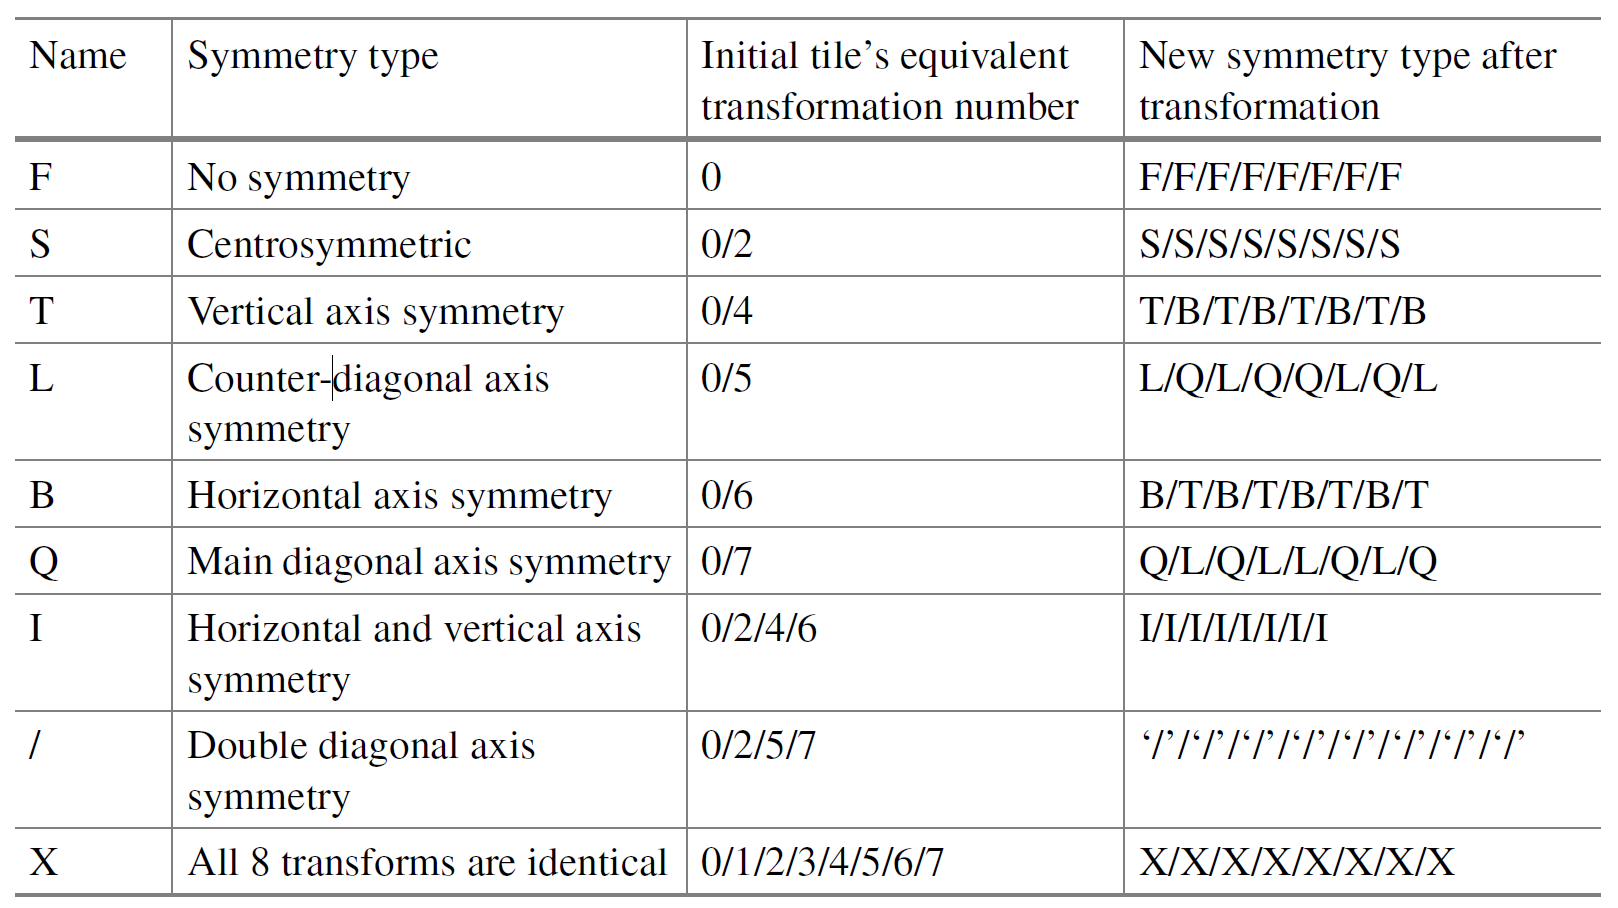
\includegraphics[width=\textwidth, height=0.3\textheight, keepaspectratio]{Images/SymmetryDictionary.png}
    \caption{A symmetry dictionary, proposed by \cite{WFC_Automatic_Rules_And_Better_Symmetries}}
    \label{fig:symmetryDictionary}
\end{table}

%\subsection{Search Algorithms}
%\subsection{Generation Methods}
%There are many different generation methods used in PCG, each with specific applications. For example, a cellular automata or agent-based digger may be used to generate a dungeon or cave. Noise maps [CITE] are often used for terrain generators such as the one used in Minecraft [CITE].
 % First draft
\chapter{Requirements Specification}
The following objectives were outlined in the Description, Objectives, Ethics and Resources (DOER) document at the start of the project. Primary objectives were chosen as core requirements of the project, with secondary objectives serving as additional goals if time allowed.
\subsection*{Primary Objectives}
\begin{itemize}
    \item Create a game that uses procedural level generation.
    \item Use novel PCG methods such as Wave Function Collapse.
    \item Extend on at least one PCG method.
    \item Use assets to give the game a full set of graphics and audio.
\end{itemize}
\subsection*{Secondary Objectives}
\begin{itemize}
    \item Make levels navigable by AI opponents.
    \item Allow customisation of level generation and other gameplay elements via an in-game menu.
\end{itemize}
 % First draft
\chapter{Software Engineering Process}
\section{Methodology}
\subsection{General Overview}
The project was carried out with use of Agile methodologies. Weekly supervisor meetings were held, in which the past week's work would be evaluated. This was then contextualised within the overall time frame of the project. This critical analysis helped to identify and set goals for the next week and beyond. Agile development suited the nature of the project as the full progression of the project was not clear from the start. For example, initially it was planned to apply a Wave Function Collapse implementation directly and focus more on extending it to aid game design. However, while there were many implementations of WFC available online, many of them had poor documentation and did not work out of the box due to missing assets and errors, while others could not be applied to a 3D tile set. The official Wave Function Collapse GitHub contains links to other WFC implementations \cite{Gumin_Wave_Function_Collapse_2016}. Four implementations investigate were the original implementation, two forks by Joseph Parker \cite{unity-WFC} and Maksim Priakhin \cite{unity-WFC-3D} as well as a simplified implementation by Garnet Kane \cite{Easy_WFC}.

\subsection{Semester One}
% How meetings were held.
% What meetings consisted of.
% How what was discussed in meetings changed over time. I.e. earlier meetings consisted of... Second semester consisted of... This problem came up. I did this to solve it... (STAR)
The key areas of focus in the first semester were carrying out a literature review, setting objectives, reviewing ethics, designing the game and implementing the WFC algorithm. As described, the goal of the project was initially to extend upon an existing implementation of WFC. As this was unsuccessful, the focus changed to implementing an algorithm from scratch. After the core of the constraint solver was finished, WFC's lowest entropy cell selection and random weighted tile selection were added. The meeting notes for semester one are available in appendix section \ref{sec:semester_one_meeting_notes}.

\subsection{Semester Two}
The key areas of focus in the second semester were finishing the game and documenting the project in this report. The core generation had already been fully implemented, but assets still had to be created and put into the generator. Furthermore, extensions on the constraint solver, such as infinite modifying in blocks and starting block constraints, had to be added to make levels infinite and playable. Additional work during the holidays involved studying infinite modifying in blocks, adding graphics filters and starting block modelling. A list of tasks was created during this time and extended during semester two. This list and the meeting notes for semester two are available in appendix sections \ref{sec:tasks} and \ref{sec:semester_two_meeting_notes} respectively.

\section{Tools and Technologies}
\subsection{Unity (C\#)}
Unity was used as the game engine for development. This was chosen as Unity and its scripting API language C\# have commonly been used for implementations of Wave Function Collapse, including the original WFC repository by Maxim Gumin \cite{Gumin_Wave_Function_Collapse_2016}. WFC has also been adapted to other engines such as Unreal Engine \cite{unreal_engine_WFC}. Two issues that faced later development using Unity were its poor support for multithreading and importing \texttt{.fbx} models from Blender.

\subsection{Blender}
Blender was used to create tile models. Each model could be created and textured before being exported as \texttt{.fbx} files. These were then imported into Unity and unpacked. They could then be used as GameObjects and have any additional assets such as lights and audio sources attached.

\subsection{GitHub}
GitHub was used for version control. This was useful for comparing new and old code and tracking progress over time.

\subsection{Document Management}
Google Drive and Google Docs, both part of Google Workspace, were used to hold most documents relating to the project. This included a tasks document, game design document, weekly meeting notes, literature review research document and credits document for any external resources used. Furthermore, Overleaf was used to write up this report. These online platforms enabled work from multiple locations and more effective evaluation with the project supervisor as the latest versions of documents were always available. % Partial first draft
\chapter{Ethics}
There are no ethical considerations. All questions on the self-assessment form could be answered with ``No''. This included the following declarations:
\begin{itemize}
    \item The project did not use any secondary datasets.
    \item The project did not involve research with human subjects.
    \item No potential physical or psychological harm, discomfort or stress to researchers or participants was foreseeable.
    \item No conflicts of interest arose in the project.
    \item The project was not externally funded.
    \item The project did not involve the use of living animals.
\end{itemize} % First draft
\chapter{Design}
% Indicating the structure of the system, with particular focus on main ideas of the design, unusual design features, etc.
% Describe the design of your program. Justify the decisions you made.
%%%%%%%%%%%%%%%%%%%%%%%%%%%%%%%%%%%%%%%\section{JUSTIFY DECISIONS!!!!!!!!!!}
\section{Game Design}
\subsection{Premise}
The premise of the game was inspired by the fictional concept of \textit{the Backrooms}. These encompass an endless collection of `levels', each a potentially infinite space with a unique theme centred around invoking a feeling of liminality. This was deemed a suitable theme to use for a game exploring novel \acrlong{pcg} techniques. The first level of \textit{the Backrooms}, `Level Zero', resembles an empty office-like space. Yellow wallpaper, light brown carpet and bright fluorescent lights combine to give it an unsettling monotone appearance and soundscape.

% Side-by-side Image of the backrooms with image in-game

\subsection{Gameplay}
\subsubsection{Player Controller}
The player controller was taken from an online tutorial \cite{FPS_controller_YouTube, FPS_controller_GitHub}. Additionally, the ability to pick up and drop items was added. This allows the player to solve puzzles throughout the world.

%\subsubsection{Puzzles}
%The player must explore the Backrooms in search of items spawned randomly with the level geometry.

% REMEMBER: COLLECT ITEMS TO REPAIR SOMETHING!
% Goal walls are locked doors. Adjacent to them are fuse boxes?

% Old idea (?):
% Goal walls are locked doors. Safe in wall containing key. Safe requires finding combination / power out?


%\begin{enumerate}
%\item Find 
%\end{enumerate}

\section{Level Generation}
\subsection{Contextualising the Wave Function Collapse Algorithm}
The \acrfull{wfc} algorithm can be viewed as an extension on the ideas presented by the \acrfull{mac3} algorithm. What is referred to as a grid of cells with tile choices in \acrlong{wfc} is analogous to a graph of variables / nodes with a domain of possible values. Constraints between variables can then be viewed as edges in an undirected graph (Figure \ref{fig:undirectedGraph}).

% Diagram of a directed graph

\begin{figure}[H]
    \centering
    \subfigure[Undirected graph]{
        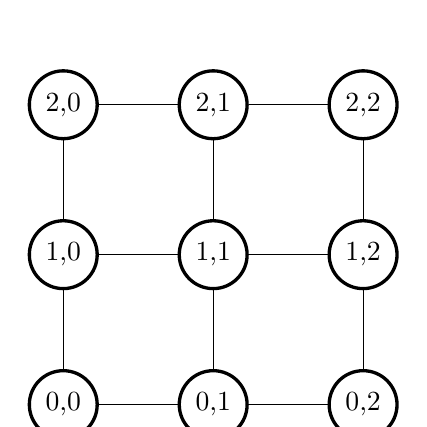
\begin{tikzpicture}[circlenode/.style={circle, draw=black, very thick, minimum size=5mm}]
            %Nodes
            \node[circlenode]      (00)                              {0,0};
            \node[circlenode]      (01)       [right=of 00]          {0,1};
            \node[circlenode]      (02)       [right=of 01]          {0,2};
            \node[circlenode]      (10)       [above=of 00]          {1,0};
            \node[circlenode]      (11)       [right=of 10]          {1,1};
            \node[circlenode]      (12)       [right=of 11]          {1,2};
            \node[circlenode]      (20)       [above=of 10]          {2,0};
            \node[circlenode]      (21)       [right=of 20]          {2,1};
            \node[circlenode]      (22)       [right=of 21]          {2,2};

            %Lines
            \draw[-] (00.north) -- (10.south);
            \draw[-] (10.north) -- (20.south);
            \draw[-] (01.north) -- (11.south);
            \draw[-] (11.north) -- (21.south);
            \draw[-] (02.north) -- (12.south);
            \draw[-] (12.north) -- (22.south);

            \draw[-] (00.east) -- (01.west);
            \draw[-] (01.east) -- (02.west);
            \draw[-] (10.east) -- (11.west);
            \draw[-] (11.east) -- (12.west);
            \draw[-] (20.east) -- (21.west);
            \draw[-] (21.east) -- (22.west);
        \end{tikzpicture}
        \label{fig:undirectedGraph}
    }
    \hfill
    \subfigure[Directed graph]{
        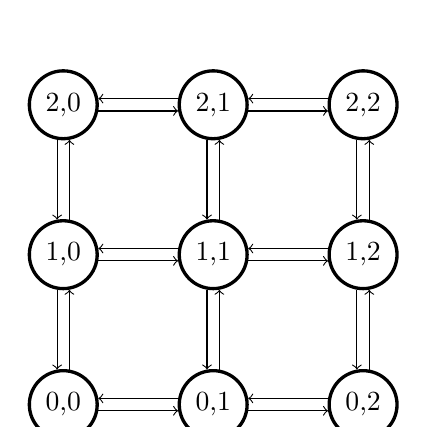
\begin{tikzpicture}[circlenode/.style={circle, draw=black, very thick, minimum size=5mm}]
            %Nodes
            \node[circlenode]      (00)                              {0,0};
            \node[circlenode]      (01)       [right=of 00]          {0,1};
            \node[circlenode]      (02)       [right=of 01]          {0,2};
            \node[circlenode]      (10)       [above=of 00]          {1,0};
            \node[circlenode]      (11)       [right=of 10]          {1,1};
            \node[circlenode]      (12)       [right=of 11]          {1,2};
            \node[circlenode]      (20)       [above=of 10]          {2,0};
            \node[circlenode]      (21)       [right=of 20]          {2,1};
            \node[circlenode]      (22)       [right=of 21]          {2,2};

            %Lines

            \draw[->] (00.800) -- (10.280);
            \draw[->] (10.800) -- (20.280);
            \draw[->] (01.800) -- (11.280);
            \draw[->] (11.800) -- (21.280);
            \draw[->] (02.800) -- (12.280);
            \draw[->] (12.800) -- (22.280);

            \draw[<-] (00.100) -- (10.260);
            \draw[<-] (10.100) -- (20.260);
            \draw[<-] (01.100) -- (11.260);
            \draw[<-] (11.100) -- (21.260);
            \draw[<-] (02.100) -- (12.260);
            \draw[<-] (12.100) -- (22.260);

            \draw[->] (00.350) -- (01.190);
            \draw[->] (01.350) -- (02.190);
            \draw[->] (10.350) -- (11.190);
            \draw[->] (11.350) -- (12.190);
            \draw[->] (20.350) -- (21.190);
            \draw[->] (21.350) -- (22.190);

            \draw[<-] (00.370) -- (01.170);
            \draw[<-] (01.370) -- (02.170);
            \draw[<-] (10.370) -- (11.170);
            \draw[<-] (11.370) -- (12.170);
            \draw[<-] (20.370) -- (21.170);
            \draw[<-] (21.370) -- (22.170);
        \end{tikzpicture}
        \label{fig:directedGraph}
    }

    \caption{A \(3\times3\) cell grid as an undirected and directed graph}
    \label{fig:graphs}
\end{figure}

\subsection{Arcs}
An edge in an undirected graph can alternatively be viewed as two opposite edges in a directed graph (Figure \ref{fig:directedGraph}). Arcs apply this concept to constraints, with each arc representing one of the two edges making up a constraint in the directed graph. For an arc to be locally arc consistent, all the values in the first variable's domain must be supported by at least one value in the second variable's domain.

For example, suppose the use of an extremely simple tile set with only cubes and empty tiles, where any tile choice is possible at the start. Furthermore, say that cubes can only have other cubes as neighbours and that empty tiles only have empty tiles as neighbours. This corresponds to Figure \ref{fig:arcsStart}.

\begin{figure}[H]
    \centering
    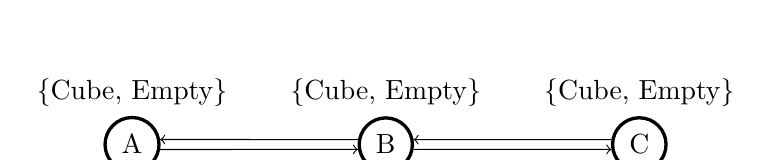
\begin{tikzpicture}[circlenode/.style={circle, draw=black, very thick, minimum size=5mm}]
        %Nodes
        \node[circlenode, label={[align=center]\{Cube, Empty\}}]      (00)                                            {A};
        \node[circlenode, label={[align=center]\{Cube, Empty\}}]      (01)       [right=of 00, xshift=1.5cm]          {B};
        \node[circlenode, label={[align=center]\{Cube, Empty\}}]      (02)       [right=of 01, xshift=1.5cm]          {C};

        %Lines
        \draw[->] (00.350) -- (01.190);
        \draw[<-] (00.370) -- (01.170);
        \draw[->] (01.350) -- (02.190);
        \draw[<-] (01.370) -- (02.170);
    \end{tikzpicture}
    \caption{Example starting state, in which all arcs are consistent}
    \label{fig:arcsStart}
\end{figure}

Then, assume that node A is set to be a cube, removing the empty tile from its domain. Now, the arc <A,B> is consistent as B still has a cube as a support value. However, the arc <B,A> is no longer consistent since the empty tile does not have any support in A's domain, which only has the cube in it. This corresponds to Figure \ref{fig:arcsAssigned}.

% Diagram showing two arcs of a constraint
\begin{figure}[H]
    \centering
    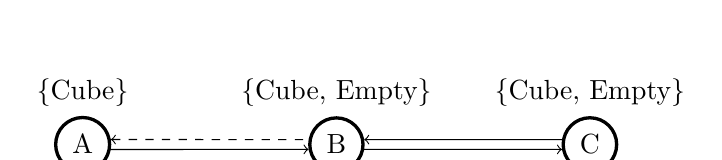
\begin{tikzpicture}[circlenode/.style={circle, draw=black, very thick, minimum size=5mm}]
        %Nodes
        \node[circlenode, label={[align=center]\{Cube\}}]      (00)                                            {A};
        \node[circlenode, label={[align=center]\{Cube, Empty\}}]      (01)       [right=of 00, xshift=1.5cm]          {B};
        \node[circlenode, label={[align=center]\{Cube, Empty\}}]      (02)       [right=of 01, xshift=1.5cm]          {C};

        %Lines
        \draw[->] (00.350) -- (01.190);
        \draw[<-, dashed] (00.370) -- (01.170);
        \draw[->] (01.350) -- (02.190);
        \draw[<-] (01.370) -- (02.170);
    \end{tikzpicture}
    \caption{After assigning Cube to A, <B,A> is no longer consistent}
    \label{fig:arcsAssigned}
\end{figure}

\subsection{AC3}
The \acrfull{ac3} algorithm enforces arc consistency in the grid of cells. The algorithm is given a queue of arcs to enforce arc consistency across. Each arc is checked for support and unsupported domain values pruned. If any domain changes occur, then all arcs targeting the primary variable of the current arc are re-added to the queue. This is required as the domain change may have resulted in support for arcs to this variable being lost.

% Diagram showing arc revision
Back to the example, assigning Cube to A will trigger arc revision with all the arcs incident on A. In this case, this initialises the queue with arc <B,A>. Checking the arc shows that B's Empty value is no longer supported by A (Figure \ref{fig:arcRevision}).

\begin{figure}[H]
    \begin{framed}
        \begin{enumerate}
            \item Check arc <B,A>:
                  \begin{enumerate}
                      \item B's value Cube has support in A through its value Cube.
                      \item B's value Empty does NOT have support in A! Remove it from the domain.
                  \end{enumerate}
        \end{enumerate}
    \end{framed}
    \caption{Revising arc <B,A>}
    \label{fig:arcRevision}
\end{figure}

Performing this single revision leaves the graph in the state as shown in Figure \ref{fig:arcsRevised1}. Revising <B,A> results in <C,B> becoming inconsistent, highlighting the importance of adding targeted arcs to the queue after a domain change. In this case, <C,B> must be added to the queue. <A,B> does not have to be added since the domain change happened while revising <B,A>. This exploits the fact that arc support is bi-directional, meaning that if a value is supported on <B,A>, then it must be supporting some value on arc <A,B>.

\begin{figure}[H]
    \centering
    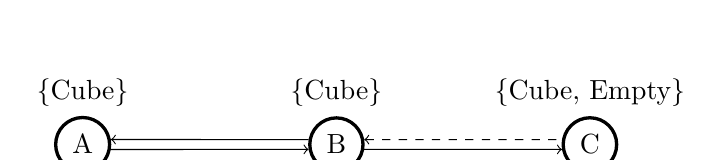
\begin{tikzpicture}[circlenode/.style={circle, draw=black, very thick, minimum size=5mm}]
        %Nodes
        \node[circlenode, label={[align=center]\{Cube\}}]      (00)                                            {A};
        \node[circlenode, label={[align=center]\{Cube\}}]      (01)       [right=of 00, xshift=1.5cm]          {B};
        \node[circlenode, label={[align=center]\{Cube, Empty\}}]      (02)       [right=of 01, xshift=1.5cm]          {C};

        %Lines
        \draw[->] (00.350) -- (01.190);
        \draw[<-] (00.370) -- (01.170);
        \draw[->] (01.350) -- (02.190);
        \draw[<-,dashed] (01.370) -- (02.170);
    \end{tikzpicture}

    \caption{Revising <B,A> results in <C,B> becoming inconsistent}
    \label{fig:arcsRevised1}
\end{figure}

Revision of <C,B> proceeds similarly to revision of <B,A> (Figure \ref{fig:arcRevision}). Similarly, C's domain change from revision of <C,B> does not require re-checking of arc <B,C>. After this, the queue of arcs to revise is empty and as such the consistency before assignment has been maintained. The state after revision is shown in Figure \ref{fig:arcsRevised2}.

\begin{figure}[H]
    \centering
    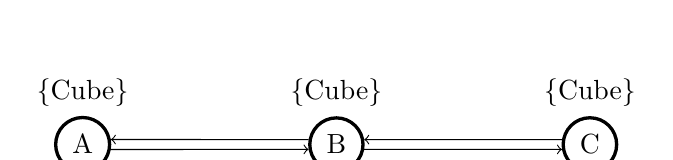
\begin{tikzpicture}[circlenode/.style={circle, draw=black, very thick, minimum size=5mm}]
        %Nodes
        \node[circlenode, label={[align=center]\{Cube\}}]      (00)                                            {A};
        \node[circlenode, label={[align=center]\{Cube\}}]      (01)       [right=of 00, xshift=1.5cm]          {B};
        \node[circlenode, label={[align=center]\{Cube\}}]      (02)       [right=of 01, xshift=1.5cm]          {C};

        %Lines
        \draw[->] (00.350) -- (01.190);
        \draw[<-] (00.370) -- (01.170);
        \draw[->] (01.350) -- (02.190);
        \draw[<-] (01.370) -- (02.170);
    \end{tikzpicture}

    \caption{The graph after \acrshort{ac3} has been carried out}
    \label{fig:arcsRevised2}
\end{figure}

An additional property to note is that each node now only has one value in its domain. Given that each arc is consistent, this means that this is a valid solution to the original problem where each node could either be a cube or empty tile. In the context of \acrshort{wfc}, this means that all cells have been collapsed with a valid tile choice and thus that a valid map has been generated.

\subsection{MAC3}
\acrfull{mac3} uses \acrfull{ac3} to create a full constraint solving algorithm. To begin, \acrshort{ac3} is run with all arcs to ensure global arc consistency at the start. Then, a variable and value are chosen in an attempt to find a solution. This choice is like that done in the example shown previously in Figure \ref{fig:arcsAssigned}. Arc consistency is then maintained by running \acrshort{ac3} with the all the arcs targeting the variable that had a value assigned (Figure \ref{fig:arcRevision}). This ensures that these arcs maintain local arc consistency. As global arc consistency was enforced at the start, maintaining local arc consistency after each assignment is enough to also maintain global arc consistency. If any variable assignments lead to a domain wipeout (an empty domain) when enforcing arc consistency, then backtracking can be performed and another value chosen. Once each variable only has one value left and all arcs are consistent, a solution has been found. If not stopped by a timeout, \acrshort{mac3} will continue running until a solution has been found or all choices have been attempted, meaning that there is no solution.

Sudoku can serve as an example to make the constraint solving process clearer. Someone solving Sudoku might pencil in the possible number for each cell to help make guesses and fill the grid.

At the start, given numbers help the player pencil each remaining cell. Like this, the possible numbers of each cell are reduced. If a cell only has one possible number remaining, then the player knows that the cell must hold that value. This is analogous to running \acrshort{ac3} at the start to ensure each cell has a consistent set of possible numbers.

Eventually, the player is likely to face the situation where no more numbers can be inferred from the given clues. Just like the \acrshort{mac3} solver, the player must make a guess as to what the correct number might be. After making a guess, the implications of it can be carried forward. This is analogous to running \acrshort{ac3} after making a variable assignment.

If this guess was incorrect and leads to a cell with no choices remaining, the player must undo the guess. This is analogous to having a domain wipeout and backtracking. After backtracking, the player knows that the choice they made was incorrect, so can pencil out the number they tried. From this, they may gain more clues about other cells in the grid. This is analogous to unassigning a value and running \acrshort{ac3} again.

If the player keeps making guesses and inferring additional information from them, they will eventually solve the Sudoku. If the player were to ignore the implications of a guess, then their solution may not be valid. This highlights the need to maintain consistency between each pair of constrained cells in the grid.

\subsection{Variable and Value Choice}\label{sec:variableAndValueChoice}
The manner in which a variable and value are chosen can be implemented as desired. The most effective method often depends on the specific problem. A common method used in \acrlong{wfc} is lowest entropy cell selection together with weighted random tile selection.

\subsubsection{Lowest Entropy Cell Selection}
The lowest entropy method can be viewed as choosing the most constrained cell at each step as it takes into account the weight of each cell. This increases the chance to find a solution quickly as any contradictory assignments are reached faster and backtracked from with fewer steps. The weight of each tile is defined in the level editor and represents the target rate of occurrence of a tile in the generated level. Equation \ref{shannonEntropy} shows the Shannon Entropy of a cell, which is lowest for cells with a small number of remaining tile choices of imbalanced weighting.% An example of this concept is shown in figure \ref{fig:entropyExample}.

% https://robertheaton.com/2018/12/17/wavefunction-collapse-algorithm/ - At latest 26.02.2024, but definitely before then.
\begin{align}
    \label{shannonEntropy}
    \text{Shannon Entropy}=S=\log(\sum{\text{weight}}) - \frac{\sum\left(\text{weight} \times \log(\text{weight})\right)}{\sum{\text{weight}}}
\end{align}

% Cell selection image. Show how lowest entropy selects the most constrained cell.
%\begin{figure}[H]
%\centering
%\includegraphics[width=\textwidth, height=0.3\textheight, keepaspectratio]{ImagePath}
%\caption{captionText}
%\label{fig:entropyExample}
%\end{figure}

\subsubsection{Weighted Random Tile Selection}
Once a cell has been chosen, the tile choice is done by summing all tile weights and then choosing a random number within that range. This gives higher weight tiles a higher chance to be selected. If the tile choice did not include any randomness, then unplayable levels such as a completely empty level could be generated. This highlights the challenge in applying a simple constraint solver to level generation in a game. A level that satisfies all constraints for the solver does not necessarily translate to a good level. Some additional constraints could be added in, such as requiring a specific block in generated chunks. However, other constraints such as requiring a certain percentage of a specific block type in the entire level are harder to enforce effectively and efficiently. Such constraints can be encourage implicitly in generation, through features such as the weighted random tile selection. With this, output is not guaranteed to satisfy block percentages, but instead strongly biased towards creating outputs that roughly match these constraints. Figure \ref{fig:weights} shows how different tile weight configurations can create vastly different levels. Careful tweaking of weights is required to create an appealing level. Having too dense of a level can create inaccessible areas as in Figure \ref{fig:weights3}.
% Should parts of the above be moved to evaluation or somewhere else?

% Show screenshots of how varying weights produces different levels.
\begin{figure}[H]
    \centering
    \subfigure[Increased weights for empty tiles creates a sparser level]{
        \includegraphics[width=0.95\textwidth, height=0.3\textheight, keepaspectratio]{Images/WeightsSparse.jpg}
        \label{fig:weights1}
    }

    \subfigure[A balance of weights for all tiles creates a level with some sparse and some dense areas]{
        \includegraphics[width=0.95\textwidth, height=0.3\textheight, keepaspectratio]{Images/WeightsNormal.jpg}
        \label{fig:weights2}
    }

    \subfigure[Increasing weights for solid tiles creates a denser level, with increasing chance of unreachable areas]{
        \includegraphics[width=0.95\textwidth, height=0.3\textheight, keepaspectratio]{Images/WeightsDense.jpg}
        \label{fig:weights3}
    }
    \caption{Examples of levels with three different tile weight configurations}
    \label{fig:weights}
\end{figure}

\subsection{Infinite Modifying in Blocks}
\label{sec:IMIB}
\acrlong{imib} works by splitting up generation into overlapping chunks, each of which are split into four layers. These layers are offset such that they do not interfere with each other. This can be used to ensure that generation is deterministic and optionally process each layer in parallel.% As example, the images in Figure \ref{} show the concept in action. The images from the original source were edited to show more clearly the concepts of chunks and layers as implemented.

% Diagram of chunks.

The algorithm is run layer by layer, finishing the layers of all active chunks before moving to the next layer. First, a layer is prepared. This involves calculating the area inside of the chunk that forms the layer and clearing all cells inside of it.

% Show first layer preparation.

Second, the solver tries to find a solution for the layer. This takes into account adjacency information from the cells next to the layer. If a solution is not found, the layer is left as it was before. This is not an issue for most tile sets as single layer failures are hidden by other layers successfully generating.

% Single layer generated.

Once each chunk has generated its first layer, the second layer is generated. This process is repeated until all layers have been generated.

% Images of all layers generating.

\section{Graphics}
\subsection{Models and Textures}
The models with texturing for each tile were made in the software Blender using a YouTube video as a guide \cite{backroomsGraphics}. The tiles have distinct shapes, but share common wallpaper \cite{sketchfab_texture}, ceiling tile \cite{ceiling_texture} and carpet textures \cite{carpet_texture}. These textures are mapped so that they appear continuous when tiles are placed next to each other. Each of the models used is shown in Figure \ref{fig:blenderTileSet}. From left to right, the models include a cube, corner, corner pillar, wall, centre pillar and empty tile.

% Image of tiles in Blender. Write text to define each.
\begin{figure}[H]
    \centering
    \includegraphics[width=\textwidth, height=0.3\textheight, keepaspectratio]{Images/Tileset.jpg}
    \caption{The model tile set in Blender}
    \label{fig:blenderTileSet}
\end{figure}

\subsection{Visual Effects}
Unity's Universal Render Pipeline was used to give additional control over rendering and visual effects. To simulate the appearance of a video recorded onto a VHS tape, a range of camera effects were used. These are listed in Figure \ref{fig:cameraEffects}.

\begin{figure}[H]
    \begin{framed}
        \begin{itemize}
            \item Depth of Field: Blurs objects that are very close to the camera, simulating depth.
            \item Bloom: Increases the effect of light on the scene, emulating high sensitivity.
            \item Motion Blur: Simulates unclear image capture from moving the camera.
            \item Tonemapping (ACES): Maps colour tones differently to give a filmic effect, making the image appear more realistic.
            \item Lens Distortion: Shifts projection around the centre of the image to simulate capture through a lens.
            \item Film Grain: Adds noise to the image to simulate similar noise real cameras can capture.
            \item Chromatic Aberration: Disperses red, green and blue colours at the edge of the screen to simulate the same effect lenses can exhibit in real life.
            \item Panini Projection: Shifts projection to better render perspective views in wide angle scenes. Acts as additional distortion to make the image appear more organic.
            \item Color Adjustments: Reduces exposure to make tones more neutral. Also adds a colour filter to shift colours slightly more towards monochrome yellow to fit the level theme.
            \item Fog: Obscures distant objects to hide the border of currently generated chunks.
        \end{itemize}
    \end{framed}
    \caption{Camera Effects}
    \label{fig:cameraEffects}
\end{figure}

\subsection{Lighting Model}
A deferred lighting model was used to light the level \cite{lighting_models}. Unity's default lighting relies heavily on baked lighting to provide for high quality lighting. Baking lighting describes pre-calculating lighting before runtime. Textures can then be illuminated cheaply at runtime using this baking data to help give levels a realistic look.

% Example of baked lighting

As the project uses procedurally generated levels, it must heavily rely on realtime lighting instead. This describes lighting that is calculated at runtime as opposed to baked lighting. However, forward rendering (Unity's default rendering method) only allows for a limited number of realtime light sources to be rendered at once. Deferred lighting instead supports many realtime lights at the cost of less accurate lighting.

% Compare two images. One is forward rendering of a generated level and the other deferred.

\section{Audio}
To give the game area an immersive soundscape, a collection of ambient effects and sound effects were used. Ambient effects are those sounds that are played equally at all times, while sound effects are those sounds that are placed inside of the environment. The most distinct sound effect of Level Zero of the Backrooms is the buzzing of the fluorescent lights. Each empty tile with a light is given an audio source that plays such a sound. Each light is given its own random offset so that the audio does not poorly overlap and cause constructive interference. For ambient sounds, a VHS sound and low droning are included. All audio assets were taken from \url{freesound.org} as this site offers sounds free for use in games.

\section{Unity Editor and Tile Representation}
The Unity Editor was used to provide a platform with which level designer could specify parameters for level generation. First, the level designer should attach the Level Generation Manager component to a unity game object. The designer may specify the size of chunks use in \acrlong{imib}. Tiles are split into three different components across the entire specification to generation pipeline, with the tile set for generation specified in steps 1 and 2.
\begin{enumerate}
    \item The level designer must first specify tiles by creating Unity game objects and then attaching a subclass of the Tile component to it. The Cube subclass exists for fully-symmetric tiles and the NonSymmetric subclass exists for all other tiles. The designer can then specify tile adjacencies by dragging other tile game objects into the neighbours arrays and specifying the desired rotation of the neighbouring tile. Base rotations of tiles should have their solid face at the back of the tile. The base rotation for corner tiles has the back of the corner on the left and back of the tile. Each game object should then be dragged into the tile set array of the level generator. Additionally, an empty tile must be specified directly.
    \item After specifying tile adjacencies, the level designer should import FBX models to form a second set of game objects. These should be given a collider to avoid the player falling through the level. The designer can also add any additional components such as lights or audio sources. These model game objects can then be referenced in the matching tile script component. This tells the level generator to use the desired model for a given tile. The tile size specified in the level generator must match the size of the tile models in order for the generator to put them together properly.
    \item Finally, the tile set that the level designer specified is converted from the designer-specified semi-explicit tile set to a fully-explicit tile set. The level generator takes each specified tile and rotates it in steps of 90 degrees, adjusting adjacency data to suit. This gives each possible rotation of a tile its own tile, hence the term fully-explicit. In effect, this enables the generation of maps without having to perform intermediate calculations on tile rotation, simplifying the algorithm at the cost of a larger tile set.
\end{enumerate}

% Diagram of specification to generation pipeline. Define cardinality / rotation clearly in the diagram. Maybe also in text more clearly or somewhere else. % Partially written
\chapter{Implementation}
% How the implementation was done and tested, with particular focus on important / novel algorithms and/or data structures, unusual implementation decisions, novel user interface features, etc.
% General Introduction: Language used. How it linked to the task. How the task progressed over time. Any changes over time.
% Specific Sections: Goal of each part. Purpose or context within larger whole. How each part works step by step. (STAR?)
\section{Cells}
\subsection{Cell Class}\label{sec:cellClass}
The cell class contains integer coordinates, a set of possible tile options and a tile prefab game object. These variables allow the cell to be used in a grid for level generation. The set of tile options is initialised with the entire fully-explicit tile set. As WFC is run on a grid including the cell, tiles that become invalid options are removed. Once the cell has been collapsed, the assigned tile is instantiated. Additionally a reference to the instantiated tile is preserved in the tile prefab field.

% Diagram of a Cell, showing its list of possible tile choices.
\begin{figure}[H]
    \centering
    \subfigure[Cell]{
        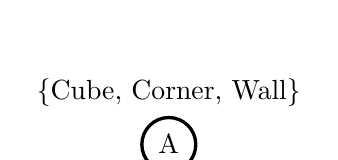
\begin{tikzpicture}[circlenode/.style={circle, draw=black, very thick, minimum size=5mm}]
            %Nodes
            \node[circlenode, label={[align=center]\{Cube, Corner, Wall\}}]      (00)                                            {A};

            %Lines
        \end{tikzpicture}
        \label{fig:tileOptions1}
    }

    \vspace{\baselineskip} % add some vertical space between the rows

    \subfigure[Cube Tile]{
        \includegraphics[width=0.2375\textwidth, height=0.1\textheight, keepaspectratio]{Images/CubeTile.png}
        \label{fig:tileOptions2}
    }
    \hfill
    \subfigure[Corner Tile]{
        \includegraphics[width=0.2375\textwidth, height=0.1\textheight, keepaspectratio]{Images/CornerTile.png}
        \label{fig:tileOptions3}
    }
    \hfill
    \subfigure[Wall Tile]{
        \includegraphics[width=0.2375\textwidth, height=0.1\textheight, keepaspectratio]{Images/WallTile.png}
        \label{fig:tileOptions4}
    }
    \caption{A cell with cube, corner and wall tiles as options}
    \label{fig:tileOptions}
\end{figure}

One additional property to note is that the cell class does not inherit from Unity's MonoBehaviour class. This means that it can use constructors that pass basic information needed to initialise each cell. Initialisation data includes the coordinates of the cell within the current layer, the cell's global grid coordinates and the current chunk using the cell. This data is needed for constraint calculations while solving and is updated each time a new layer is spawned.

Objects that do inherit from MonoBehaviour cannot use constructors safely and must instead use Unity's Start or Awake functions. However, the Start and Awake functions cannot easily be passed initialisation data. The cost of not inheriting from MonoBehaviour is that any such instances cannot be attached to any objects spawned in the world.

\subsection{CellArc Class}
The cell arc class is used to represent arcs in the grid. Each arc contains references to two cells. The constructor is used to ensure that the arc is valid. This is done by comparing the x and y coordinates of the cells when creating the arc. An exception is thrown when the cells are not adjacent. Cells being adjacent is specific to the context of WFC. In Sudoku, for example, a pair of constrained cells need not be directly adjacent.

% Show two cells and their arc.

\subsection{CellReference Class}\label{sec:cellReferenceClass}
The cell reference class contains a reference to a cell. As mentioned in Section \ref{sec:cellClass}, the cell class does not inherit from MonoBehaviour and as such cannot be attached to any objects in the world. By instead inheriting from MonoBehaviour, a cell reference instance can be attached to a tile. Having this cell reference attached to a tile allows the cell's data to be used in generation of later layers.

% Screenshot of CellReference on generated tile in Unity?

\section{Tiles}
\subsection{Rotation / Cardinality}
Each spawned tile has a cardinality of either 0, 1, 2 or 3. These cardinalities correspond to rotations of 0, 90, 180 and 270 degrees respectively. As example, all cardinalities for the corner tile are shown in Figure \ref{fig:cornerCardinalities}.

% Show corner tile with cardinalities 0, 1, 2 and 3.\begin{figure}[H]
\begin{figure}[H]
    \centering
    \subfigure[Cardinality 0 (0 Degrees)]{
        \rotatebox[origin=c]{-0}{
            \includegraphics[width=0.2375\textwidth, height=0.1\textheight, keepaspectratio]{Images/CornerTile.png}
        }
        \label{fig:cornerCardinalities0}
    }
    \hfill
    \subfigure[Cardinality 1 (90 Degrees)]{
        \rotatebox[origin=c]{-90}{
            \includegraphics[width=0.2375\textwidth, height=0.1\textheight, keepaspectratio]{Images/CornerTile.png}
        }
        \label{fig:cornerCardinalities1}
    }
    \hfill
    \subfigure[Cardinality 2 (180 Degrees)]{
        \rotatebox[origin=c]{-180}{
            \includegraphics[width=0.2375\textwidth, height=0.1\textheight, keepaspectratio]{Images/CornerTile.png}
        }
        \label{fig:cornerCardinalities2}
    }
    \hfill
    \subfigure[Cardinality 3 (270 Degrees)]{
        \rotatebox[origin=c]{-270}{
            \includegraphics[width=0.2375\textwidth, height=0.1\textheight, keepaspectratio]{Images/CornerTile.png}
        }
        \label{fig:cornerCardinalities3}
    }
    \caption{The corner tile with all possible rotations (counted clockwise)}
    \label{fig:cornerCardinalities}
\end{figure}

Cardinality information is used to determine which combination of two tiles and their rotations fit together. For example, a single wall tile constituting part of a longer wall will require any adjacent wall tiles to be of the same cardinality as in Figure \ref{fig:wallExample1}. When specifying the neighbours of a tile, the level designer must also set the cardinality of each neighbour.

% Also show wall tiles fitting together. 0,0,0 walls fit and 3,0,1 walls don't.
\begin{figure}[H]
    \centering
    \subfigure[Valid wall placement (Cardinalities 0,0,0,0)]{
        \includegraphics[width=0.2375\textwidth, height=0.1\textheight, keepaspectratio]{Images/WallTile.png}
        \includegraphics[width=0.2375\textwidth, height=0.1\textheight, keepaspectratio]{Images/WallTile.png}
        \includegraphics[width=0.2375\textwidth, height=0.1\textheight, keepaspectratio]{Images/WallTile.png}
        \includegraphics[width=0.2375\textwidth, height=0.1\textheight, keepaspectratio]{Images/WallTile.png}
        \label{fig:wallExample1}
    }

    \vspace{\baselineskip} % add some vertical space between the rows

    \subfigure[Invalid wall placement (Cardinalities 3,0,2,1)]{
        \rotatebox[origin=c]{-270}{
            \includegraphics[width=0.2375\textwidth, height=0.1\textheight, keepaspectratio]{Images/WallTile.png}
        }
        \rotatebox[origin=c]{-0}{
            \includegraphics[width=0.2375\textwidth, height=0.1\textheight, keepaspectratio]{Images/WallTile.png}
        }
        \rotatebox[origin=c]{-180}{
            \includegraphics[width=0.2375\textwidth, height=0.1\textheight, keepaspectratio]{Images/WallTile.png}
        }
        \rotatebox[origin=c]{-90}{
            \includegraphics[width=0.2375\textwidth, height=0.1\textheight, keepaspectratio]{Images/WallTile.png}
        }
        \label{fig:wallExample2}
    }
    \caption{Comparison of valid wall placement to invalid wall placement if adjacent walls must have matching cardinality}
    \label{fig:wallExample}
\end{figure}

\subsection{Tile Symmetry}\label{sec:tileSymmetry}
To reduce the amount of adjacency data to be specified by the level designer, as well as the chance for human error, the level generator includes the functionality to convert a semi-explicit tile set into a fully-explicit tile set. This fully-explicit tile set is created at the start of generation in several steps.

First, it is checked whether the empty tile was specified and is included in the semi-explicit tile set. After confirming this, the main conversion stage begins.

Second, a non-symmetric copy is created for each tile. Non-symmetric tiles may have different neighbours on each side. Any symmetric tile can be represented as a non-symmetric tile. For example, a tile with equal symmetry on all sides can be converted by copying the single list of neighbours onto all sides and incrementing the cardinality per side as required. Specifically, cardinalities on side 1 are incremented by 1, those on side 2 by 2 and those on side 3 by 3. This fully symmetric tile is called a cube tile in the code.

% Image of cube with wall neighbour being turned into non-symmetric tile.
\begin{figure}[H]
    \subfigure[A symmetric cube tile with only a wall neighbour of cardinality 2 on the back side specified]{
        \begin{minipage}[b]{0.45\linewidth}
            \centering
            \rotatebox[origin=c]{-180}{
                \includegraphics[width=0.2375\textwidth, height=0.1\textheight, keepaspectratio]{Images/WallTile.png}
            }

            \includegraphics[width=0.2375\textwidth, height=0.1\textheight, keepaspectratio]{Images/CubeTile.png}

            \includegraphics[width=0.2375\textwidth, height=0.1\textheight, keepaspectratio]{Images/EmptyTile.png}
        \end{minipage}
        \label{fig:cubeSymmetryConversion1}
    }
    \hfill
    \subfigure[A non-symmetric cube tile variant with a wall neighbour specified on each side. Clockwise from the back, cardinalities of the walls are 2, 3, 0 and 1.]{
        \begin{minipage}[b]{0.45\linewidth}
            \centering
            \rotatebox[origin=c]{-180}{
                \includegraphics[width=0.2375\textwidth, height=0.1\textheight, keepaspectratio]{Images/WallTile.png}
            }

            \rotatebox[origin=c]{-90}{
                \includegraphics[width=0.2375\textwidth, height=0.1\textheight, keepaspectratio]{Images/WallTile.png}
            }
            \includegraphics[width=0.2375\textwidth, height=0.1\textheight, keepaspectratio]{Images/CubeTile.png}
            \rotatebox[origin=c]{-270}{
                \includegraphics[width=0.2375\textwidth, height=0.1\textheight, keepaspectratio]{Images/WallTile.png}
            }

            \rotatebox[origin=c]{-0}{
                \includegraphics[width=0.2375\textwidth, height=0.1\textheight, keepaspectratio]{Images/WallTile.png}
            }
        \end{minipage}
        \label{fig:cubeSymmetryConversion2}
    }
    \caption{A symmetric cube tile converted to a non-symmetric tile. For simplicity, the cube is only shown with a wall as its possible neighbour.}
    \label{fig:cubeSymmetryConversion}
\end{figure}

Third, an array for each possible tile rotation is created (cardinalities 0, 1, 2 and 3). This array is attached to the original tile to set explicit neighbours later. The instantiated tile is used as the base rotation (cardinality 0) and referenced in the array. For cube tiles, the base rotation tile can be referenced for each rotation instead of having to create additional copies. The filled in array for cube tiles is shown in Figure \ref{fig:cubeRotationsArray}.

% Show the rotations array for the cube tile and how it is just the same in each slot.
\begin{figure}[H]
    \subfigure[Cube Tile Explicit Variant 0]{
        \begin{minipage}[b]{0.22\linewidth}
            \centering
            \rotatebox[origin=c]{-180}{
                \includegraphics[width=0.2375\textwidth, height=0.1\textheight, keepaspectratio]{Images/WallTile.png}
            }

            \rotatebox[origin=c]{-90}{
                \includegraphics[width=0.2375\textwidth, height=0.1\textheight, keepaspectratio]{Images/WallTile.png}
            }
            \includegraphics[width=0.2375\textwidth, height=0.1\textheight, keepaspectratio]{Images/CubeTile.png}
            \rotatebox[origin=c]{-270}{
                \includegraphics[width=0.2375\textwidth, height=0.1\textheight, keepaspectratio]{Images/WallTile.png}
            }

            \rotatebox[origin=c]{-0}{
                \includegraphics[width=0.2375\textwidth, height=0.1\textheight, keepaspectratio]{Images/WallTile.png}
            }
        \end{minipage}
        \label{fig:cubeRotationsArray0}
    }
    \hfill
    \subfigure[Cube Tile Explicit Variant 1]{
        \begin{minipage}[b]{0.22\linewidth}
            \centering
            \rotatebox[origin=c]{-180}{
                \includegraphics[width=0.2375\textwidth, height=0.1\textheight, keepaspectratio]{Images/WallTile.png}
            }

            \rotatebox[origin=c]{-90}{
                \includegraphics[width=0.2375\textwidth, height=0.1\textheight, keepaspectratio]{Images/WallTile.png}
            }
            \includegraphics[width=0.2375\textwidth, height=0.1\textheight, keepaspectratio]{Images/CubeTile.png}
            \rotatebox[origin=c]{-270}{
                \includegraphics[width=0.2375\textwidth, height=0.1\textheight, keepaspectratio]{Images/WallTile.png}
            }

            \rotatebox[origin=c]{-0}{
                \includegraphics[width=0.2375\textwidth, height=0.1\textheight, keepaspectratio]{Images/WallTile.png}
            }
        \end{minipage}
        \label{fig:cubeRotationsArray1}
    }
    \hfill
    \subfigure[Cube Tile Explicit Variant 2]{
        \begin{minipage}[b]{0.22\linewidth}
            \centering
            \rotatebox[origin=c]{-180}{
                \includegraphics[width=0.2375\textwidth, height=0.1\textheight, keepaspectratio]{Images/WallTile.png}
            }

            \rotatebox[origin=c]{-90}{
                \includegraphics[width=0.2375\textwidth, height=0.1\textheight, keepaspectratio]{Images/WallTile.png}
            }
            \includegraphics[width=0.2375\textwidth, height=0.1\textheight, keepaspectratio]{Images/CubeTile.png}
            \rotatebox[origin=c]{-270}{
                \includegraphics[width=0.2375\textwidth, height=0.1\textheight, keepaspectratio]{Images/WallTile.png}
            }

            \rotatebox[origin=c]{-0}{
                \includegraphics[width=0.2375\textwidth, height=0.1\textheight, keepaspectratio]{Images/WallTile.png}
            }
        \end{minipage}
        \label{fig:cubeRotationsArray2}
    }
    \hfill
    \subfigure[Cube Tile Explicit Variant 3]{
        \begin{minipage}[b]{0.22\linewidth}
            \centering
            \rotatebox[origin=c]{-180}{
                \includegraphics[width=0.2375\textwidth, height=0.1\textheight, keepaspectratio]{Images/WallTile.png}
            }

            \rotatebox[origin=c]{-90}{
                \includegraphics[width=0.2375\textwidth, height=0.1\textheight, keepaspectratio]{Images/WallTile.png}
            }
            \includegraphics[width=0.2375\textwidth, height=0.1\textheight, keepaspectratio]{Images/CubeTile.png}
            \rotatebox[origin=c]{-270}{
                \includegraphics[width=0.2375\textwidth, height=0.1\textheight, keepaspectratio]{Images/WallTile.png}
            }

            \rotatebox[origin=c]{-0}{
                \includegraphics[width=0.2375\textwidth, height=0.1\textheight, keepaspectratio]{Images/WallTile.png}
            }
        \end{minipage}
        \label{fig:cubeRotationsArray3}
    }
    \caption{The array of explicit variants for the cube tile with neighbours shown. Due to the tile's symmetry, no extra work is needed to calculate variants for cardinalities 1, 2 and 3.}
    \label{fig:cubeRotationsArray}
\end{figure}

For non-cube tiles, variants for the remaining cardinalities (1, 2 and 3) must be created. Each new variant copies the previous one. This allows a loop to be used that always performs 90 degree steps. First, the tile is rotated by 90 degrees. Then, neighbour data and rotation arrays are swapped. This sets back neighbours as left neighours, left neighbours as front neighbours and so on. Finally, the cardinality values of all neighbours are incremented by 1 to mark the 90 degree rotation. The filled in array for corner tiles is shown in Figure \ref{fig:cornerRotationsArray}.

% Show the rotations array for the corner tile. Show cardinality 0 corner rotated to cardinality 1 corner etc.
\begin{figure}[H]
    \subfigure[Corner Tile Explicit Variant 0]{
        \begin{minipage}[b]{0.22\linewidth}
            \centering
            \includegraphics[width=0.2375\textwidth, height=0.1\textheight, keepaspectratio]{Images/CubeTile.png}

            \includegraphics[width=0.2375\textwidth, height=0.1\textheight, keepaspectratio]{Images/CubeTile.png}
            \includegraphics[width=0.2375\textwidth, height=0.1\textheight, keepaspectratio]{Images/CornerTile.png}
            \includegraphics[width=0.2375\textwidth, height=0.1\textheight, keepaspectratio]{Images/WallTile.png}

            \rotatebox[origin=c]{-270}{
                \includegraphics[width=0.2375\textwidth, height=0.1\textheight, keepaspectratio]{Images/WallTile.png}
            }
        \end{minipage}
        \label{fig:cornerRotationsArray0}
    }
    \hfill
    \subfigure[Corner Tile Explicit Variant 1]{
        \begin{minipage}[b]{0.22\linewidth}
            \centering
            \includegraphics[width=0.2375\textwidth, height=0.1\textheight, keepaspectratio]{Images/CubeTile.png}

            \includegraphics[width=0.2375\textwidth, height=0.1\textheight, keepaspectratio]{Images/WallTile.png}
            \rotatebox[origin=c]{-90}{
                \includegraphics[width=0.2375\textwidth, height=0.1\textheight, keepaspectratio]{Images/CornerTile.png}
            }
            \includegraphics[width=0.2375\textwidth, height=0.1\textheight, keepaspectratio]{Images/CubeTile.png}

            \rotatebox[origin=c]{-90}{
                \includegraphics[width=0.2375\textwidth, height=0.1\textheight, keepaspectratio]{Images/WallTile.png}
            }
        \end{minipage}
        \label{fig:cornerRotationsArray1}
    }
    \hfill
    \subfigure[Corner Tile Explicit Variant 2]{
        \begin{minipage}[b]{0.22\linewidth}
            \centering
            \rotatebox[origin=c]{-90}{
                \includegraphics[width=0.2375\textwidth, height=0.1\textheight, keepaspectratio]{Images/WallTile.png}
            }

            \rotatebox[origin=c]{-180}{
                \includegraphics[width=0.2375\textwidth, height=0.1\textheight, keepaspectratio]{Images/WallTile.png}
            }
            \rotatebox[origin=c]{-180}{
                \includegraphics[width=0.2375\textwidth, height=0.1\textheight, keepaspectratio]{Images/CornerTile.png}
            }
            \includegraphics[width=0.2375\textwidth, height=0.1\textheight, keepaspectratio]{Images/CubeTile.png}

            \includegraphics[width=0.2375\textwidth, height=0.1\textheight, keepaspectratio]{Images/CubeTile.png}
        \end{minipage}
        \label{fig:cornerRotationsArray2}
    }
    \hfill
    \subfigure[Corner Tile Explicit Variant 3]{
        \begin{minipage}[b]{0.22\linewidth}
            \centering
            \rotatebox[origin=c]{-270}{
                \includegraphics[width=0.2375\textwidth, height=0.1\textheight, keepaspectratio]{Images/WallTile.png}
            }

            \includegraphics[width=0.2375\textwidth, height=0.1\textheight, keepaspectratio]{Images/CubeTile.png}
            \rotatebox[origin=c]{-270}{
                \includegraphics[width=0.2375\textwidth, height=0.1\textheight, keepaspectratio]{Images/CornerTile.png}
            }
            \rotatebox[origin=c]{-180}{
                \includegraphics[width=0.2375\textwidth, height=0.1\textheight, keepaspectratio]{Images/WallTile.png}
            }

            \includegraphics[width=0.2375\textwidth, height=0.1\textheight, keepaspectratio]{Images/CubeTile.png}
        \end{minipage}
        \label{fig:cornerRotationsArray3}
    }
    \caption{The array of explicit variants for the corner tile with neighbours shown.}
    \label{fig:cornerRotationsArray}
\end{figure}

These explicit variants do not yet have tile rotation implicitly encoded in their neighbour data. The original tile neighbours in the tile array must be replaced with their explicit variants matching the rotations in the rotations array. To do this, the array assigned to each tile containing all the explicit variants is used once all explicit variants have been created. For each neighbour of the explicit tile, the reference to the non-explicit neighbour is replaced by the explicit neighbour with the correct orientation. As example, the explicit corner tile variants are shown with the original cube and wall neighbours in Figure \ref{fig:explicitNeighbourUpdate}. The references are changed to explicit cube and wall neighbours to match Figure \ref{fig:cornerRotationsArray}.

% Diagram of this process. Show the original tile and each variant in a line. Then show how the neighbours of one of these is replaced with the explicit variants.
\begin{figure}[H]
    \subfigure[Corner Tile Explicit Variant 0 Before Neighbour Update]{
        \begin{minipage}[b]{0.22\linewidth}
            \centering
            \includegraphics[width=0.2375\textwidth, height=0.1\textheight, keepaspectratio]{Images/CubeTile.png}

            \includegraphics[width=0.2375\textwidth, height=0.1\textheight, keepaspectratio]{Images/CubeTile.png}
            \includegraphics[width=0.2375\textwidth, height=0.1\textheight, keepaspectratio]{Images/CornerTile.png}
            \includegraphics[width=0.2375\textwidth, height=0.1\textheight, keepaspectratio]{Images/WallTile.png}

            \includegraphics[width=0.2375\textwidth, height=0.1\textheight, keepaspectratio]{Images/WallTile.png}
        \end{minipage}
        \label{fig:explicitNeighbourUpdate0}
    }
    \hfill
    \subfigure[Corner Tile Explicit Variant 1 Before Neighbour Update]{
        \begin{minipage}[b]{0.22\linewidth}
            \centering
            \includegraphics[width=0.2375\textwidth, height=0.1\textheight, keepaspectratio]{Images/CubeTile.png}

            \includegraphics[width=0.2375\textwidth, height=0.1\textheight, keepaspectratio]{Images/WallTile.png}
            \rotatebox[origin=c]{-90}{
                \includegraphics[width=0.2375\textwidth, height=0.1\textheight, keepaspectratio]{Images/CornerTile.png}
            }
            \includegraphics[width=0.2375\textwidth, height=0.1\textheight, keepaspectratio]{Images/CubeTile.png}

            \includegraphics[width=0.2375\textwidth, height=0.1\textheight, keepaspectratio]{Images/WallTile.png}
        \end{minipage}
        \label{fig:explicitNeighbourUpdate1}
    }
    \hfill
    \subfigure[Corner Tile Explicit Variant 2 Before Neighbour Update]{
        \begin{minipage}[b]{0.22\linewidth}
            \centering
            \includegraphics[width=0.2375\textwidth, height=0.1\textheight, keepaspectratio]{Images/WallTile.png}

            \includegraphics[width=0.2375\textwidth, height=0.1\textheight, keepaspectratio]{Images/WallTile.png}
            \rotatebox[origin=c]{-180}{
                \includegraphics[width=0.2375\textwidth, height=0.1\textheight, keepaspectratio]{Images/CornerTile.png}
            }
            \includegraphics[width=0.2375\textwidth, height=0.1\textheight, keepaspectratio]{Images/CubeTile.png}

            \includegraphics[width=0.2375\textwidth, height=0.1\textheight, keepaspectratio]{Images/CubeTile.png}
        \end{minipage}
        \label{fig:explicitNeighbourUpdate2}
    }
    \hfill
    \subfigure[Corner Tile Explicit Variant 3 Before Neighbour Update]{
        \begin{minipage}[b]{0.22\linewidth}
            \centering
            \includegraphics[width=0.2375\textwidth, height=0.1\textheight, keepaspectratio]{Images/WallTile.png}

            \includegraphics[width=0.2375\textwidth, height=0.1\textheight, keepaspectratio]{Images/CubeTile.png}
            \rotatebox[origin=c]{-270}{
                \includegraphics[width=0.2375\textwidth, height=0.1\textheight, keepaspectratio]{Images/CornerTile.png}
            }
            \includegraphics[width=0.2375\textwidth, height=0.1\textheight, keepaspectratio]{Images/WallTile.png}

            \includegraphics[width=0.2375\textwidth, height=0.1\textheight, keepaspectratio]{Images/CubeTile.png}
        \end{minipage}
        \label{fig:explicitNeighbourUpdate3}
    }
    \caption{The explicit corner tile variants before updating neighbours to their explicit forms}
    \label{fig:explicitNeighbourUpdate}
\end{figure}

% // Initialise the explicit tile set if it has not already been done.
% // Ensure that the empty tile is in the tile set.
% // Create a game object to hold the explicit tile set.
% // Create non-symmetric variants for each tile.
% // Create a non-symmetric copy of the original tile.
% // Add the copy to the explicit tile set and set it as the 0 rotation variant.
% // Set the explicit variant of the empty tile if applicable.
%%%IF // Create rotation variants for non-cube tiles.
% // Create a rotation variant with the previous rotation as the base.
% // Rotate the variant by 90 degrees and specify its rotation / cardinality in the name.
% // Add the variant to both the tile's variants array and the explicit tile set.
% // Switch the neighbour and rotation arrays to follow the 90 degree rotation.
% // Increase cardinality values of neighbours to account for the 90 degree rotation.
%%%ELSE // For cube tiles, simply set the explicit rotation variants to be the 0 rotation non-symmetric tile.
% // Replace the neighbours of each explicit tile without explicit rotational information with explicit variants accounting for the rotations.
% // Use 2D arrays of the neighbours and rotations to simplify the operation.
% // Go through each neighbour array and neighbour tile in it.
% // Get the rotation / cardinality value of the variant to use.
% // Set the neighbour to the explicit variant with the correct rotation.

\subsection{Collapsing Cells}\label{sec:collapsingCells}
To collapse a tile into a cell, the tile's model is instantiated. Then, the model is set to follow the level generation manager's transform (position, rotation and scale) and has its local position reset to the cell's world coordinates. Doing the placement in this way ensures that the model lines up with the world grid while maintaining the correct scale and rotation. Finally, a Unity box collider is added to the model, a second reference to the tile added to the cell and the model activated to render it in the world. The second reference ensures that the spawned tile can be recovered if the generation of a layer fails. Unity's `Physics.OverlapBox' function can be used to detect the box collider given the world coordinates of the cell. This box overlap can be used to obtain the cell reference during the generation of later layers.

% Diagram of the pipeline.
% Instantiate, place, add collider, reference and set active.

\section{Chunks}
Chunks are defined by their own chunk coordinates, which are converted from world coordinates using the chunk size as a divisor. From this, each of the chunk's four layers can be defined. Layer one is aligned with the chunk's world coordinates, while layer two is offset by half a chunk in the x direction. Layer three is similarly offset by half a chunk in the y direction, while layer four is offset both in the x and y directions. Each layer is given its own layer spawner instance, which runs WFC on the portion of the chunk defined by the layer.

% Chunk diagram with layer shown.

Each chunk has its own Random Number Generator (RNG), which is used by the layer spawners when making tile choices. The seed for the RNG is defined deterministically through the chunk's coordinates. The global level generation seed is added to allow generation of multiple levels while keeping determinism. This deterministic use of RNGs when spawning chunks is what allows the level generation manager to spawn chunks identically, even when unloading and loading a chunk again.

\section{Level Generation Manager}
\subsection{Prerequisites}
To start generation, the level designer must have defined a tile set for the generator to use. This must contain an empty tile and be convertible into an explicit tile set as detailed in Section \ref{sec:tileSymmetry}.

\subsection{Solver (Layer Spawners)}
The MAC3 solver code is held in the layer spawner class. This matches the idea of layers and chunks modifying the world in an infinite set of blocks. To allow accurate placement of tiles in the world, a starting cell coordinate must be passed when initialising the layer spawner. Furthermore, a reference to the layer's parent chunk is kept in order to utilise its random number generator.

\subsection{Grid Initialisation}
First, a grid of cells is initialised. Additionally, a list of cells left to assign is initialised to simplify cell choices when solving. Padding on the layer size is used to include any previously collapsed cells. Added cells that have not been collapsed are treated as empty tiles. This padding means that non-padded cells take into account full adjacency information. If the layer were not padded, then border cells would not have arc consistency with cells outside of the layer as these arcs would not be checked by the solver. The non-padding cells in the centre of the grid are refreshed by restoring each cell's tile options set to include all possible tiles. This allows each each layer to re-generate its cells. In effect, this connects singular, overlapping layers into an infinite, continuous grid.% WHY Are non-collapsed cells treated as empty tiles? DOES THIS HELP STITCHING? EXPERIMENT AGAIN AND WRITE DOWN REASONING.

\subsection{Dealing with an Infinite Grid}
Were every cell stored in a global grid, then it would be trivially easy to get previously collapsed cells. This is unfeasible due to the requirement of letting the player navigate an infinite world. As such, once cells are collapsed, the grid used by the solver is discarded. Instead, the cell reference class described in Section \ref{sec:cellReferenceClass} is used to preserve a reference to the cell. Each tile has its own collider that can be used to obtain the cell reference as described in Section \ref{sec:collapsingCells}.% DISCUSS ALTERNATIVE IN EVALUATION. MAYBE A "SEMI-GLOBAL" GRID THAT CONTAINS ALL THE CURRENTLY COLLAPSED CELLS AND SHIFTS AS THE PLAYER MOVES.

\subsection{Setting up MAC3}
With the layer's grid fully initialised, the main stage of the solver can now begin. First, a stack of state changes is initialised. This tracks changes to cells after each assignment by pushing a new state change to the stack. To make the grid globally arc consistent, the arc of each cell in the grid is generated. Subsequently, AC3 is run with this starting queue of cell arcs.

\subsection{MAC3 Recursion}
After this, the first iteration of a recursive implementation of the MAC3 algorithm is called. Pseudocode of this is given below. How each step works and its purpose is explained in more detail in subsections following the pseudocode.

\begin{enumerate}
    \item If all cells have been assigned, return.
    \item Choose a cell and tile to assign as in Section \ref{sec:variableAndValueChoice}.
    \item Enter a new state and assign the tile to the cell, pruning other tiles from its tile options set.
    \item If the cell's tile options set changed, run AC3.
    \item Recurse if AC3 was not run or there was no domain wipeout during AC3.
    \item If all cells have been assigned, return.
    \item We are now in the case that a domain wipeout must have occurred. Revert the state.
    \item If the cell we tried to assign still has other options left, remove / `unassign' the tile we tried from the options, run AC3 and recurse again.
    \item If all cells have been assigned, return.
    \item We are now in the case that all possible tile values for a cell led to a wipeout. This means that an earlier choice must be to blame. Restore the tile we tried both to assign and unassign and return.
\end{enumerate}

\subsubsection{Managing State Changes}
To track state changes, each layer spawner holds a stack of state changes. After each time a new cell is chosen to be assigned, a new state is entered. A state change class is used that holds the cell being assigned and any domain changes occurring across the grid. Domain changes can happen to any cell and can consist of multiple tile changes, so a dictionary of cells to hash sets of tiles is used. To track a new state change, a new entry and hash set are added to the dictionary if required. After this, the hash set can be obtained from the dictionary through use of the cell and any tile changes added.

% Image of domain changes structure.

To revert a state, the domain changes dictionary is iterated through, with each cell having any removed tiles restored to its domain. Furthermore, the cell that was assigned in the state change is re-added to the list of cells left to assign.

\subsubsection{Assigning and Unassigning a Tile to a Cell}
Assigning a tile to a cell involves pruning all tiles except the one being assigned. These tiles are removed from the tile options set. Furthermore, each domain change is recorded in the current state changes. Finally, the assigned cell is removed from the list of cells left to assign. After this, AC3 can be run to maintain arc consistency.

% Image of assignment.

Unassigning a tile to a cell first requires the state to be reverted. After this, the opposite choice is taken. This is done by pruning only the tile choice that was previously assigned. This demonstrates the 2-way branching nature of the implementation. Rather than exploring all possible tile values in one level of search, each tile value is either assigned or unassigned.

\subsubsection{Visualising Recursion}
The recursive MAC3 method can be visualised as consisting of three parts as in Figure \ref{fig:mac3Recursion}.

\begin{figure}[H]
    \begin{framed}
        \begin{enumerate}
            \item Making a new assignment.
            \item Making the opposite assignment (``unassignment'') after the first one failed.
            \item Both assignments having failed.
        \end{enumerate}
    \end{framed}
    \caption{The three parts of the recursive MAC3 method}
    \label{fig:mac3Recursion}
\end{figure}

The finishing state of the grid is checked both before making the new assignment and after each of the assignments. This ensures that the recursion is finished immediately after consistency has been enforced from an assignment and each cell only has one value left. % Partially written
\chapter{Evaluation}
% Evaluate the success of your program against what you were asked to do.

% Reflect DIRECTLY on the points listed in the requirements specification. Make subsections or itemize for each point and comment on the extent of its completion.
\section{Against Requirements Specification}
\subsection{Primary Objectives}
\subsubsection{Create a game that uses procedural level generation}
The final project includes a very basic game in which the player can explore an infinite world generated through procedural level generation. The game is themed after \textit{the Backrooms}, a fictional concept detailing an infinite expanse of `levels'. The first of these levels, `Level Zero', is included in the game.

\subsubsection{Use novel PCG methods such as Wave Function Collapse}
\acrlong{wfc} was studied thoroughly throughout the project. \acrshort{wfc} was contextualised within theory of constraint programming and a simple-tiled implementation created using the \acrshort{mac3} algorithm with lowest entropy cell and weighted random tile selection.

\subsubsection{Extend on at least one PCG method}
Standard \acrlong{wfc} is finite in grid size and has increasing complexity with larger grid sizes. \acrshort{wfc} was extended upon through the addition of the \acrlong{imib} algorithm. This helped generate output consistently, where standard \acrshort{wfc} might require extensive backtracking in certain cases. Furthermore, it allowed \acrshort{wfc} to be applied to generate an infinite world by generating many small, finite chunks as the player moves around in the world.

\subsubsection{Use assets to give the game a full set of graphics and audio}
A small set of models were created to serve as tiles for \acrshort{wfc}. These match the design of \textit{the Backrooms} through the use of online assets. Furthermore, a basic soundscape is created with some tiles given fluorescent lamp sound effects. Ambience sound played consistently throughout the game also add to this.% Mention limitations.

\subsection{Secondary Objectives}
\subsubsection{Make levels navigable by AI opponents}
No attempts were made to introduce AI opponents to the game.

\subsubsection{Allow customisation of level generation and other gameplay elements via an in-game menu}
The final game allows the user to set the seed of the level generator and includes an option to spawn with all the required items to solve puzzles more quickly.

\section{Designer-facing Components}
\subsection{Editor Interface and Code Quality}
The final project includes an interface for level designers to run the \acrshort{wfc} implementation with their own tile set. Efforts were made to comment code clearly, which is something other \acrshort{wfc} implementations miss. This is also an issue facing the original \acrshort{wfc} implementation, which does not include any comments in its code \cite{Gumin_Wave_Function_Collapse_2016}.

\subsection{Ease of Use}
The level generation code includes exceptions that can tell the level designer what is incorrect with their setup. However, despite this additional guidance, the level generation manager interface can be confusing. Especially concepts such as cells vs tiles, tiles vs models and tile cardinality are likely to confuse users of the project's code. This problem is likely worsened since \acrshort{wfc} is often treated as a black box by people from a range of backgrounds \cite{WFC_In_The_Wild}. These users may not be experts in reading code and simply want to set up the generator with their own tile set. It is possible that these users are the likeliest to struggle with correctly setting up the level generation manager.

\section{Player-facing Components}
\subsection{Gameplay}
Players are able to explore an infinite map and solve simple puzzles to escape. While this may be interesting for a while, the experience has a significant issue with homogeneity. The low variety of models used means that the geometry of the level does not form many interesting structures. The lack of multiple levels also limits the amount of enjoyment players may get out of the game.

\subsection{Performance}
While the procedural level generation is functional, it suffers from a lack of optimisations that would make it more suitable to application for a video game. For example, chunk loading could be multi-threaded. However, implementation of this is difficult due to poor support by Unity. Furthermore, the use of Unity coroutines could be explored to let chunk loading take place across multiple frames. This would avoid lag spikes, which can be very off-putting to players. % Not written
\chapter{Conclusion}
% Summarise what you achieved, what you found difficult, and what you would like to do given more time.
% Restate the Research Problem/Objective
% Summary of Findings:
% Discussion of Implications
% Reflection on Methodology
% Addressing Research Questions/Goals
% Recommendations for Future Research
% Practical Implications and Applications
% Conclusion Statement
% Closing Remarks
% Summary

\acrfull{wfc} is limited by a lack of global constraints, poor performance and restriction to a finite grid. Furthermore, presentation of \acrshort{wfc} online often fails to acknowledge underlying constraint solving principles used by \acrshort{wfc}. This dissertation examined how these issues can be addressed and contextualised \acrshort{wfc} within theory of constraint programming.

A simple-tiled implementation of \acrshort{wfc} using the \acrfull{mac3} algorithm was presented and extended to generate infinite worlds using \acrfull{imib}. Weighted tile selection gives the level designer global control over the percentage of each tile in the output level. These concepts are demonstrated in a game themed after the popular fictional concept of \textit{the Backrooms}. These additions to \acrshort{wfc} show that the lack of global constraints and restriction to a finite grid can be addressed. The included game and generation interface illustrate the potential application of \acrshort{wfc} with these additions to video games.

However, loading infinite worlds in real-time presents additional performance challenges and further global constraints are needed to improve control further. The solver could be optimised through the addition of multi-threading and lazy loading across frames. Furthermore, code could be reworked to more efficiently carry generation data across layers. The ease of use of the generation interface in the Unity Editor could be improved by making it simpler to specify a tile set for generation in the Unity Editor. The game could be further developed through the addition of more models and levels.

In summary, this dissertation contextualised \acrshort{wfc} within theory of constraint programming and addressed \acrshort{wfc}'s limitations through \acrshort{imib} and weighted tile selection, extending generation to an infinite space and applying this in a game themed after \textit{the Backrooms}.

% OLD CONCLUSION
% Summarise what you achieved
%The final project includes a simple game and designer tool for creating infinite worlds using \acrlong{wfc}.

% What you found difficult
%Implementing \acrlong{wfc} and extending it with \acrlong{imib} presented a huge technical challenge. Ultimately, this detracted from work on the game itself. % Move to general evaluation with discussion about title change.

% What you would like to do given more time
%Key areas of further development are identified in Figure \ref{fig:futureGoals}.

%\begin{figure}[H]
%\begin{framed}
%\begin{itemize}
%\item Solver optimisation: Add multi-threading and lazy loading across frames to avoid lag spikes. Also, rework code to more efficiently carry generation data across layers.
%\item Ease of use for designers: Make it simpler to specify a tile set for generation in the Unity Editor.
%\item Added variety to game: Add more models to the existing level and add additional levels.
%\end{itemize}
%\end{framed}
%\caption{Key areas of further development}
%\label{fig:futureGoals}
%\end{figure} % Not written
\printbibliography
%TC:ignore - Starts ignoring word count.
\appendix
\chapter{Testing Summary}
% Describe how you tested your program. Include any ways you made sure that your program is complete and works correctly.

\chapter{Player Guide}
\subsubsection{Premise}
% Explore an infinite, procedurally generated interpretation of the Backrooms! Try to find a way out, traversing a liminal space

Embark on an infinite journey through the enigmatic depths of the Backrooms. Take in the eerie solitude in this procedurally generated liminal space, where the boundaries between reality and the unknown blur into obscurity. Scavenge for any items left behind and piece together an escape at the elusive escape points scattered throughout. Will you manage to find an exit, or will you become lost forever in this maze of yellow hues and buzzing lights?

% Image of backrooms in-game.

% AI Text 1: Embark on an endless journey through the enigmatic depths of the Backrooms, where each corridor holds a new mystery waiting to be unraveled. In this procedurally generated world, solitude envelops you as you navigate through the eerie confines of this liminal space. Your objective: find the elusive escape points scattered throughout, piecing together clues and gathering essential items along the way. Will you brave the unknown, or succumb to the labyrinthine depths of the Backrooms? The choice is yours in this haunting adventure of exploration and survival.

% AI Text 2: Embark on an infinite odyssey through the ever-shifting corridors of the Backrooms, where every step brings forth a new enigma to unravel. Delve into the eerie solitude of this procedurally generated realm, where the boundaries between reality and the unknown blur into obscurity. Your quest is clear: navigate the labyrinthine passages, scavenge for crucial resources, and decipher cryptic clues to uncover the elusive escape routes scattered throughout. Will you muster the courage to confront the mysteries lurking within, or will you become lost amidst the haunting depths of the Backrooms? The choice rests with you in this gripping tale of exploration and survival.

\subsubsection{Controls}
\begin{center}
    \begin{minipage}{0.5\textwidth}
        \begin{itemize}
            \item[Mouse:] Look
            \item[Left Mouse Button:] Use Item
            \item[Right Mouse Button:] Drop Item
            \item[Left Shift:] Run
            \item[WASD Keys:] Move
            \item[F Key:] Pick Up Item
        \end{itemize}
    \end{minipage}
\end{center}

\chapter{User Manual}
% Describe how to use the Unity Editor with screenshots and any advanced mechanics not discussed in the Player Guide.


% MEETING NOTES
\chapter{Meeting Notes}\label{sec:meeting_notes}
\section{Semester One Meeting Notes}
\label{sec:semester_one_meeting_notes}
\noindent Weeks 0 to 3
\begin{itemize}
    \item Research and narrowing down project aims.
    \item DOER and ethics submissions.
\end{itemize}
\noindent Week 4 - 03.10.2023
\begin{itemize}
    \item Create a design outline document.
    \item Try to adapt one of the WFC implementations to 3D.
    \begin{itemize}
        \item \url{https://github.com/GarnetKane99/WaveFunctionCollapse}
        \item Up, down, right, left, front, back neighbours.
        \item Each prefab in the neighbours array should have a weighting too. Use an entropy calculation.
    \end{itemize}
    \item Get a simple, one-room playable demo.
\end{itemize}

\noindent Week 5 - 10.10.2023
\begin{itemize}
    \item No meeting ILW.
    \item Adapt research into a draft context / literature review for the final report (see email for lit rev guide).
    \item Get WFC working with weights by the next meeting.
\end{itemize}

\noindent Week 7 - 24.10.2023
\begin{itemize}
    \item Try to finish literature and make an introduction to WFC in the report.
    \item Implement your own WFC.
\end{itemize}

\noindent Week 8 - 31.10.2023
\begin{itemize}
    \item Continue working on WFC algorithm.
\end{itemize}

\noindent Week 9 - 10.11.2023
\begin{itemize}
    \item Fix last bugs with MAC.
    \item Either get in symmetries or give each neighbour data explicitly for now to get generation working properly.
    \item Lowest entropy.
\end{itemize}

\noindent Week 10 - 17.11.2023
\begin{itemize}
    \item Implement weighting into the algorithm.
    \item Have another look at what is meant by entropy.
    \item Make notes on the directional artefacts (probably a result from overfitting / tileset neighbour bias).
\end{itemize}

\noindent Week 11 - 24.11.2023
\begin{itemize}
    \item Visual debugger to help with artefacts (diagonal, edge only shapes...)
    \item Refocus a bit on the game element (texturing, filter, ...)
    \item Extra: Infinite modifying in blocks, sub-wfc.
\end{itemize}

\section{Semester Two Meeting Notes}
\label{sec:semester_two_meeting_notes}
\noindent Week 1 - 17.01.2024
\begin{itemize}
    \item Goal block
    \item Have player start in middle of grid with empty blocks around at start of generation.
    \item Look more into the lighting. Replace placeholder carpet and roof. Check performance of tiling roof.
\end{itemize}

\noindent Week 2 - 24.01.2024
\begin{itemize}
    \item Main Goals:
    \begin{itemize}
        \item Continue working towards chunk generation.
        \begin{itemize}
            \item Let chunks that are separately generated overlap information.
            \begin{itemize}
                \item Chunks have trouble generating. Maybe the overlap method is not fully correct. Think about overlap size and simply getting information vs delete some part.
                \item Infinite modifying in blocks with good chunk sizes might help without backtracking.
            \end{itemize}
            \item Allow backtracking for chunks.
        \end{itemize}
        \item Script goal to let player win.
        \begin{itemize}
            \item Detect when the player touches the goal.
            \item Show a message and go back to the menu / teleport the player somewhere else.
        \end{itemize}
    \end{itemize}
    \item Extra:
    \begin{itemize}
        \item Add in a mini sub-region to test (i.e freezer).
        \item Think about making a variant for empty vs empty light.
        \item Graphics improvements:
        \begin{itemize}
            \item Fog / render distance if needed later.
            \begin{itemize}
                \item Adjusted fog colour.
                \item Should anything else be adjusted? For now, no render distance cust. needed.
            \end{itemize}
            \item Make vhs effect screen space rather than plane.
            \begin{itemize}
                \item Seems to be difficult to overlay onto the render texture without more cameras.
            \end{itemize}
            \item Skybox lighting for ambient light.
            \item Balance light settings and bloom a bit more.
        \end{itemize}
        \item Audio improvements:
        \begin{itemize}
            \item Script the lights to have random offset.
            \begin{itemize}
                \item Should probably also replace the buzz with something that doesn’t tick.
            \end{itemize}
            \item Add VHS SFX to the player.
        \end{itemize}
    \end{itemize}
\end{itemize}

\noindent Week 3 - 31.01.2024
\begin{itemize}
    \item Only discussed progress per email.
    \item Implement infinite modifying in blocks for next week.
\end{itemize}

\noindent Week 4 - 07.02.2024
\begin{itemize}
    \item Do report writing.
    \item Polish game and finish any 90\% implemented features.
    \item ((Test performance of 2D grid vs linear grid. Might be changed automatically by C\#. Probably done automatically))
\end{itemize}

\noindent Week 5 - 15.02.2024
\begin{itemize}
    \item Focussing more on other projects at the moment.
    \item Tried to do parallelisation, but it wasn’t simple. Focus on other things first.
    \begin{itemize}
        \item Generate the level as the player moves about.
    \end{itemize}
    \item Continue report writing when able.
\end{itemize}

\noindent Week 6 - 22.02.2024
\begin{itemize}
    \item Very busy with other courseworks.
    \item Continue the report in chunks over the break.
\end{itemize}


% DESIGN DOCUMENT
\chapter{Design Document}\label{sec:designDocument}
\section*{Outline}
\begin{itemize}
    \item Backrooms-style game using Wave Function Collapse (WFC) to infinitely generate rooms.
    \item Different tilesets can be used to generate different levels.
\end{itemize}

\section*{Generator}
\begin{itemize}
    \item First generate a fixed size level of a few tiles. Later, generate in chunks (modifying in infinite blocks) to support infinite generation as well as with more tiles.
    \item Generate geometry for each level. Give “doors” a weighting to go into another sub-level.
    \item Is it worth integrating some more traditional methods? Traditional generators may work better for rooms. Something more random like WFC might work better for Backrooms.
\end{itemize}

\section*{Modules / Blocks}
\begin{itemize}
    \item Each a 1x1 tile, Empyrion style block with adjacency constraints and weighting (how?) for each.
    \begin{itemize}
        \item Full
        \begin{itemize}
            \item Floor (full with carpet on top)
            \item Ceiling (full with ceiling on bottom)
            \item Could do all three in one block type? Or maybe use texture variations somehow.
        \end{itemize}
        \item Wall (half block)
        \begin{itemize}
            \item Crouch hole (rotated wall)
        \end{itemize}
        \item Corner (half)
        \item Corner (quarter)
        \item Thin Wall (quarter)
        \item Corner pillar (half)
        \item Corner pillar (quarter)
        \item Ceiling tiles
        \begin{itemize}
            \item A single tile consisting of multiple tiles (2x2?). Above empty, give each sub-tile a chance of of being emissive.
        \end{itemize}
        \item Empty
        \item Centre pillar
        \item Miscellaneous half block variants that fit other normal blocks for variety.
    \end{itemize}
\end{itemize}

\section*{Regions / Structure}
\begin{itemize}
    \item Make a ``door'' tile that is a floor tile with adjacencies that connect several sublevels.
    \item Is there a better way of doing this that maintains modularity?
    \item How might room structures be made while maintaining modularity?
    \begin{itemize}
        \item Not needed for some areas of the backrooms (i.e. starting area) as they are not well structured.
    \end{itemize}
    \item Use a density noise map that defines how empty or full an area of the map is. Helps give natural variety.
    \begin{itemize}
        \item Can also apply noise to lights and grunge for textures.
    \end{itemize}
\end{itemize}

\section*{Goal}
\begin{itemize}
    \item Collect key items across sublevels (and levels?) to unlock new areas / objectives (Monstrum escape route style).
\end{itemize}

\chapter{Holiday and Semester Two Task List}\label{sec:tasks}
\begin{itemize}
    \item Algorithm
    \begin{itemize}
        \item Make the algorithm visual (intermediate steps)
        \item Give control of generation to the player via keyboard when debugging.
        \item Infinite modifying in blocks
        \begin{itemize}
            \item Think about how this will affect modularity. Will implementing this mean changes to the base algorithm will be harder to make? Or will this just always work on top? It will probably work separately.
        \end{itemize}
        \item Sub-WFC
        \item Generate block variants for symmetries from the initial block.
    \end{itemize}
    \item Audio
    \begin{itemize}
        \item Get ambience sounds
        \item Footstep sounds
        \item Audio filter
    \end{itemize}
    \item Game
    \begin{itemize}
        \item Objectives
        \begin{itemize}
            \item Spawn items for objectives
            \item Spawn key locations among random generation
        \end{itemize}
        \item Set up player in Unity to start in the middle of the maze
        \item Make a menu screen to start the game.
    \end{itemize}
    \item Graphics
    \begin{itemize}
        \item Textures for each block
        \begin{itemize}
            \item Got a low res wallpaper texture and simple colour for rims. Should help performance.
            \item In the future, use AI art for some textures? (Just a possibility)
        \end{itemize}
        \item Filters for the camera
        \begin{itemize}
            \item First round of basic effects. Could probably be enhanced in quality later.
        \end{itemize}
        \item Graphics for floor and lights.
        \begin{itemize}
            \item Have a flat texture for the whole map? Or break it into block chunks too? Performance?
            \item Get proper lighting in that is also performant.
        \end{itemize}
    \end{itemize}
    \item Report
    \begin{itemize}
        \item Break into sections.
        \begin{itemize}
            \item Game design, algorithms, discuss different options and things tried, audio and graphics...
        \end{itemize}
    \end{itemize}
\end{itemize}
%TC:endignore - Ends ignoring word count.
\end{document}
% "input" does not include page break wrapping.
% "include" includes page break wrapping.
%TC:ignore - Starts ignoring word count.
%TC:endignore - Ends ignoring word count.

Tilly's Tips / Discussion:
6000 to 15000 words

Abstract
Declaration
Acknowledgements
Introduction
-- Player guide
Literature review
Methodology
Requirements specification??
Software engineering process
Design and implementation
Testing
Evaluation/Discussion

Deadline - 22 March

Abstract -200-300 words
Declaration /
Acknowledgements /
Introduction - 1000 words
-- Player guide
Literature review - 1500 words
Methodology/Software engineering process  - 700 words
Requirements specification??
Design and implementation - 2500 words
Testing - 1000 words
Evaluation/Discussion - 2000 words

(9) Abstract
(7) Declaration
(8) Acknowledgements
(3) Introduction
-- Player guide
(1) Literature review
(2) Methodology/Software engineering process
Requirements specification??
(4) Design and implementation
(5) Testing
(6) Evaluation/Discussion